%\documentclass[11pt,oneside,letterpaper,leqno]{report}
%\usepackage[utf8x]{inputenc}
%\usepackage[spanish,es-tabla]{babel}
%
%% Fuente Arial
%\usepackage[scaled]{uarial}
%\renewcommand*\familydefault{\sfdefault}
%\usepackage[T1]{fontenc}
%
%% Interlineado 1.5
%\usepackage{setspace}
%\onehalfspacing
%
%% Márgenes de Página
%\usepackage[left=4cm,top=4cm,right=2.5cm,bottom=2.5cm]{geometry}
%
%% Bibliografía en Español
%%\usepackage{babelbib}
%\usepackage[fixlanguage]{babelbib}
%\selectbiblanguage{spanish}
%
%%%%%%%%%%%%%%%%%%%% region Tablas style %%%%%%%%%%%%%%%%%%%
%\usepackage{multirow}
%\usepackage{tabularx}
%\usepackage{array}
%\newcolumntype{L}[1]{>{\raggedright\let\newline\\\arraybackslash\hspace{0pt}}m{#1}}
%\newcolumntype{C}[1]{>{\centering\let\newline\\\arraybackslash\hspace{0pt}}m{#1}}
%\newcolumntype{R}[1]{>{\raggedleft\let\newline\\\arraybackslash\hspace{0pt}}m{#1}}
%
% 
%\newcommand{\reftabla}[1]{\tablename \ref{#1}}
%%%%%%%%%%%%%%%%%%%% endregion Tablas style %%%%%%%%%%%%%%%%%%%
%
%%%%%%%%%%%%%%%%%%%% region JavaScript style %%%%%%%%%%%%%%%%%%%
%\usepackage{listings}
%\usepackage{color}
%\definecolor{lightgray}{rgb}{.9,.9,.9}
%\definecolor{darkgray}{rgb}{.4,.4,.4}
%\definecolor{purple}{rgb}{0.65, 0.12, 0.82}
%
%\lstdefinelanguage{JavaScript}{
%	keywords={typeof, new, true, false, catch, function, return, null, catch, switch, var, if, in, while, do, else, case, break},
%	keywordstyle=\color{blue}\bfseries,
%	ndkeywords={class, export, boolean, throw, implements, import, this},
%	ndkeywordstyle=\color{darkgray}\bfseries,
%	identifierstyle=\color{black},
%	sensitive=false,
%	comment=[l]{//},
%	morecomment=[s]{/*}{*/},
%	commentstyle=\color{purple}\ttfamily,
%	stringstyle=\color{red}\ttfamily,
%	morestring=[b]',
%	morestring=[b]"
%}
%
%\lstset{
%	language=JavaScript,
%	backgroundcolor=\color{lightgray},
%	extendedchars=true,
%	basicstyle=\footnotesize\ttfamily,
%	showstringspaces=false,
%	showspaces=false,
%	numbers=left,
%	numberstyle=\footnotesize,
%	numbersep=9pt,
%	tabsize=2,
%	breaklines=true,
%	showtabs=false,
%	captionpos=b
%}
%
%%Modificar el caption
%\renewcommand{\lstlistingname}{Código}
%\newcommand{\refsource}[1]{\lstlistingname \ref{#1}}
%%%%%%%%%%%%%%%%%%%% endregion JavaScript style %%%%%%%%%%%%%%%%%%%
%
%%%%%%%%%%%%%%%%%%%% region constants %%%%%%%%%%%%%%%%%%%
%
%%Names
%\newcommand{\mongodb}{\gloss{mongodb}}
%\newcommand{\nodejs}{Node.js}
%\newcommand{\javascript}{\gloss{javascript}}
%\newcommand{\ecommerce}{\gloss{ecommerce}}
%\newcommand{\express}{express}
%
%\newcommand{\json}{\gloss{json}}
%\newcommand{\sql}{\gloss{sql}}
%\newcommand{\nosql}{\gloss{nosql}}
%\newcommand{\workload}{\gloss{workload}}
%\newcommand{\rdbms}{\gloss{rdbms}}
%\newcommand{\framework}{Framework}
%\newcommand{\join}{join}
%\newcommand{\joins}{joins}
%\newcommand{\xml}{XML}
%\newcommand{\php}{PHP}
%\newcommand{\opensource}{open source}
%\newcommand{\performance}{performance}
%\newcommand{\hardware}{hardware}
%\newcommand{\software}{software}
%\newcommand{\benchmark}{benchmark}
%
%%internet
%\newcommand{\web}{web}
%\newcommand{\internet}{Internet}
%\newcommand{\www}{World Wide Web}
%\newcommand{\http}{HTTP}
%\newcommand{\https}{HTTPS}
%\newcommand{\dotcom}{dot-com}
%\newcommand{\online}{online}
%\newcommand{\offline}{offline}
%
%\newcommand{\serverside}{server-side}
%\newcommand{\clientside}{client-side}
%\newcommand{\frontend}{Front-End}
%\newcommand{\backend}{Back-End}
%
%\newcommand{\mobile}{mobile}
%\newcommand{\task}{Task}
%
%%e-commerce 
%\newcommand{\wishlist}{wish list}
%
%%Social Networks
%\newcommand{\twitter}{Twitter}
%\newcommand{\facebook}{Facebook}
%\newcommand{\foursquare}{Foursquare}
%
%%%%%%%%%%%%%%%%%%%% endregion constants %%%%%%%%%%%%%%%%%%%
%
%% Glosario
%\usepackage{gloss}
%\makegloss
%\renewcommand\glossname{Glosario}
%
%% Para PS:
%%\usepackage{pslatex}
%%\usepackage[dvips]{graphicx}
%
%% Para solo PDF:
%\usepackage[pdftex]{graphicx}
%
%\DeclareGraphicsRule{.emf}{bmp}{}{}
%\DeclareGraphicsExtensions{.pdf,.png,.jpg,.bmp,.gif} %solo para PDFLaTeX
%
%\spanishdecimal{.}
%
%\usepackage{calc}
%\usepackage{subfig}
%\usepackage{enumerate}
%\usepackage{paralist}
%\usepackage{url}
%
%%Enumerar secciones de manera particular
%\usepackage{sectsty}
%
%%Paquete de dibujo
%\usepackage{pgf}
%\usepackage{tikz}
%\usetikzlibrary{calc,shapes,arrows,decorations.pathmorphing,automata}
%\usepackage[all]{xy}
%
%%Paquete de dibujo plots 3D
%\usepackage{tikz-3dplot}
%\newcommand{\dotrule}[1]{\parbox[t]{#1}{\dotfill}}
%\usepackage{amsmath}
%\usepackage{amssymb}
%\usepackage{cite}
%\usepackage{multirow}
%\usepackage{nameref}
%\usepackage[colorlinks=true,linkcolor=black,urlcolor=black,citecolor=black]{hyperref}
%
%\DeclareMathOperator*{\argmax}{arg\,max}
%
%%Paquete para mini-Table-Of-Contents
%\usepackage{minitoc}
%
%\usepackage{algorithm}
%\usepackage{algorithmic}
%\floatname{algorithm}{Algoritmo}
%
%%para código fuente
%\newenvironment{codigoenv}
%{\fontsize{10pt}{12pt} \linespread{1}} { \normalsize}
%
%%INDENTACIÓN
%\parindent=8mm
%
%%ESPACIADO PARRAFOS
%\setlength{\parskip}{3mm}
%\setlength{\footskip}{10mm}
%\setlength{\headsep}{10mm}
%
%%Titulo para tabla de contenido pequeñas
%\def\mtctitle{Contenido}
%
%% Evitar separación de palabras
%\pretolerance=10000
%\tolerance=10000
%
%%%%%%%%%%%%%%%%%%%%%%%  DATOS MEMORIA   %%%%%%%%%%%%%%%%%%%%
%\newcommand{\memtitle}{TITLE UNKNOW}
%\newcommand{\autor}{Álvaro Balmaceda Celedón}
%\newcommand{\profesor}{Nelson Baloian}
%\newcommand{\coguia}{UNKNOW COGUIA}
%\newcommand{\integrante}{UNKNOW INTEGRANTE}
%\newcommand{\fecha}{Diciembre 2014}
%\newcommand{\tipomemoria}{INGENIERO CIVIL COMPUTACIÓN}
%\newcommand{\dpto}{DEPARTAMENTO DE CIENCIAS DE LA COMPUTACIÓN}
%
%%%%%%%%%%%%%%%%%%%%%%	COMANDOS PERSONALIZADOS		%%%%%%%%%%%%%%%%%%%%%
%\newcommand{\Memtitle}{\MakeUppercase{\memtitle}}
%\newcommand{\Author}{\MakeUppercase{\autor}}
%\newcommand{\Profesor}{\MakeUppercase{\profesor}}
%\newcommand{\Coguia}{\MakeUppercase{\coguia}}
%\newcommand{\Integrante}{\MakeUppercase{\integrante}}
%\newcommand{\Fecha}{\MakeUppercase{\fecha}}
%\newcommand{\Tipomemoria}{\MakeUppercase{\tipomemoria}}
%\newcommand{\Dpto}{\MakeUppercase{\dpto}}
%
%%%%%%%%%%%%%%%%%%%% region Figura %%%%%%%%%%%%%%%%%%%
%%%%%%%%%%% Figura  %%%%%%%%%%
%%   1: ruta imagen
%%   2: medida
%%   3: caption
%%   4: label
%%Ej: \figura{portada.png}{width=10cm}{este es el texto q va abajo de la figura}{fig:portada}
%\newcommand{\figura}[4]
%{
%   \begin{figure}[H]
%     \centering
%     \caption{#3}\label{#4}
%     \includegraphics[#2]{#1}
%   \end{figure}
%}
%
%\newcommand{\refFigura}[1]{\figurename \ref{#1}}
%%%%%%%%%%%%%%%%%%%% endregion Figura %%%%%%%%%%%%%%%%%%%
\documentclass[11pt,oneside,letterpaper,leqno]{report}
\usepackage{etex}
\usepackage[utf8]{inputenc}
\usepackage[spanish,es-tabla]{babel}

% Bibliografía en Español
%\usepackage{babelbib}
\usepackage[fixlanguage]{babelbib}
\selectbiblanguage{spanish}

% Fuente Arial
\usepackage[scaled]{uarial}
\renewcommand*\familydefault{\sfdefault}
\usepackage[T1]{fontenc}

% Interlineado 1.5
\usepackage{setspace}
\onehalfspacing

% Márgenes de Página
\usepackage[left=4cm,top=4cm,right=2.5cm,bottom=2.5cm]{geometry}

%%%%%%%%%%%%%%%%%%% region Tablas style %%%%%%%%%%%%%%%%%%%
\usepackage{multirow}
\usepackage{tabularx}
\usepackage{array}
\newcolumntype{L}[1]{>{\raggedright\let\newline\\\arraybackslash\hspace{0pt}}m{#1}}
\newcolumntype{C}[1]{>{\centering\let\newline\\\arraybackslash\hspace{0pt}}m{#1}}
\newcolumntype{R}[1]{>{\raggedleft\let\newline\\\arraybackslash\hspace{0pt}}m{#1}}




%%%%%%%%%%%%%%%%%%% endregion Tablas style %%%%%%%%%%%%%%%%%%%

%%%%%%%%%%%%%%%%%%% region JavaScript style %%%%%%%%%%%%%%%%%%%
\usepackage{listings}
\usepackage{color}
\definecolor{lightgray}{rgb}{.9,.9,.9}
\definecolor{darkgray}{rgb}{.4,.4,.4}
\definecolor{purple}{rgb}{0.65, 0.12, 0.82}

\lstdefinelanguage{JavaScript}{
	keywords={typeof, new, true, false, catch, function, return, null, catch, switch, var, if, in, while, do, else, case, break},
	keywordstyle=\color{blue}\bfseries,
	ndkeywords={class, export, boolean, throw, implements, import, this},
	ndkeywordstyle=\color{darkgray}\bfseries,
	identifierstyle=\color{black},
	sensitive=false,
	comment=[l]{//},
	morecomment=[s]{/*}{*/},
	commentstyle=\color{purple}\ttfamily,
	stringstyle=\color{red}\ttfamily,
	morestring=[b]',
	morestring=[b]"
}

\lstset{
	language=JavaScript,
	backgroundcolor=\color{lightgray},
	extendedchars=true,
	basicstyle=\footnotesize\ttfamily,
	showstringspaces=false,
	showspaces=false,
	numbers=left,
	numberstyle=\footnotesize,
	numbersep=9pt,
	tabsize=2,
	breaklines=true,
	showtabs=false,
	captionpos=b
}

%%%%%%%%%%%%%%%%%%% endregion JavaScript style %%%%%%%%%%%%%%%%%%%

% Glosario
\usepackage{gloss}
\makegloss
\renewcommand\glossname{Glosario}

% Para PS:
%\usepackage{pslatex}
%\usepackage[dvips]{graphicx}

% Para solo PDF:
\usepackage[pdftex]{graphicx}

\DeclareGraphicsRule{.emf}{bmp}{}{}
\DeclareGraphicsExtensions{.pdf,.png,.jpg,.bmp,.gif} %solo para PDFLaTeX

\spanishdecimal{.}

\usepackage{calc}
\usepackage{subfig}
\usepackage{enumerate}
\usepackage{paralist}
\usepackage{url}

%Enumerar secciones de manera particular
\usepackage{sectsty}

%Paquete de dibujo
\usepackage{pgf}
\usepackage{tikz}
\usetikzlibrary{positioning,calc,shapes,arrows,shadows,trees,decorations.pathmorphing,automata}

%Symbolo checkmark
\def\checkmark{\tikz\fill[scale=0.4](0,.35) -- (.25,0) -- (1,.7) -- (.25,.15) -- cycle;} 

\usepackage[all]{xy}

%Paquete de dibujo plots 3D
\usepackage{tikz-3dplot}
\newcommand{\dotrule}[1]{\parbox[t]{#1}{\dotfill}}
\usepackage{amsmath}
\usepackage{amssymb}
\usepackage{cite}
\usepackage{multirow}
\usepackage{nameref}
\usepackage[colorlinks=true,linkcolor=black,urlcolor=black,citecolor=black]{hyperref}

\DeclareMathOperator*{\argmax}{arg\,max}

%Paquete para mini-Table-Of-Contents
\usepackage{minitoc}

\usepackage{algorithm}
\usepackage{algorithmic}
\floatname{algorithm}{Algoritmo}

%para código fuente
\newenvironment{codigoenv}
{\fontsize{10pt}{12pt} \linespread{1}} { \normalsize}

%INDENTACIÓN
\parindent=8mm

%ESPACIADO PARRAFOS
\setlength{\parskip}{3mm}
\setlength{\footskip}{10mm}
\setlength{\headsep}{10mm}

%Titulo para tabla de contenido pequeñas
\def\mtctitle{Contenido}

% Evitar separación de palabras
\pretolerance=10000
\tolerance=10000

%%%%%%%%%%%%%%%%%%% region LayersDiagram style %%%%%%%%%%%%%%%%%%%

\definecolor{mybluei}{rgb}{.48,.6,.8}
\definecolor{myblueii}{rgb}{.28,.47,.75}
\definecolor{mygreen}{rgb}{.78,.85,.5}
\definecolor{mywhite}{rgb}{1,1,1}


\pgfdeclarelayer{background}
\pgfsetlayers{background,main}
            
%%%%%%%%%%%%%%%%%%% endregion LayersDiagram style %%%%%%%%%%%%%%%%%%%

%%%%%%%%%%%%%%%%%%% region Fix space \newcommand bug %%%%%%%%%%%%%%%%%%%
\usepackage{xspace}
%%%%%%%%%%%%%%%%%%% endregion Fix space \newcommand bug %%%%%%%%%%%%%%%%%%%
%%%%%%%%%%%%%%%%%%% region Figura %%%%%%%%%%%%%%%%%%%
%%%%%%%%%% Figura  %%%%%%%%%%
%   1: ruta imagen
%   2: medida
%   3: caption
%   4: label
%Ej: \figura{portada.png}{width=10cm}{este es el texto q va abajo de la figura}{fig:portada}
\newcommand{\figura}[4]
{
   \begin{figure}[H]
     \centering
     \caption{#3}\label{#4}
     \includegraphics[#2]{#1}
   \end{figure}
}
%%%%%%%%%%%%%%%%%%% endregion Figura %%%%%%%%%%%%%%%%%%%

%%%%%%%%%%%%%%%%%%% 		region References per caption		%%%%%%%%%%%%%%%%%%% 
% 
\newcommand{\reftabla}[1]		{\tablename \ref{#1}}

%Modificar el caption
\renewcommand{\lstlistingname}	{Código}
\newcommand{\refsource}[1]		{\lstlistingname \ref{#1}}

\newcommand{\refFigura}[1]		{\figurename \ref{#1}}
%%%%%%%%%%%%%%%%%%% 		endregion References per caption 	%%%%%%%%%%%%%%%%

\newcommand{\rootfolder}		{../../}


%%%%%%%%%%%%%%%%%%% region constants %%%%%%%%%%%%%%%%%%%

%%%%%%%%%%%%%%%%%%%%%%%%%%%%%%%%%%%%%%%%%
%										%
%			    Nombres					%
%										%
%%%%%%%%%%%%%%%%%%%%%%%%%%%%%%%%%%%%%%%%%

\newcommand{\frameworkname}		{\gloss{e_ecommerce} }
\newcommand{\chrome}			{Chrome }
\newcommand{\twitter}			{Twitter }
\newcommand{\facebook}			{Facebook }
\newcommand{\ebay}				{Ebay }
\newcommand{\amazon}			{Amazon }
\newcommand{\foursquare}			{Foursquare }
\newcommand{\mongodb}			{\gloss{mongodb} }
\newcommand{\nodejs}				{Node.js }
\newcommand{\npm}				{NPM }
\newcommand{\apttool}			{APT }
\newcommand{\clitool}			{CLI }
\newcommand{\maketool}			{make }
\newcommand{\grunttool}			{Grunt }
\newcommand{\expressjs}			{Express.js }
\newcommand{\dockerio}			{Docker.io }
\newcommand{\docker}			{Docker }
\newcommand{\coffeescript}		{CoffeeScript }
\newcommand{\linux}				{Linux }
\newcommand{\angularjs}			{Angular.js }
\newcommand{\apache}				{Apache }
\newcommand{\mysql}				{MySql }
\newcommand{\postgresql}		{PostgreSQL }
\newcommand{\sqlite}			{SQLite }
\newcommand{\emberjs}			{Ember.js }
\newcommand{\backbonejs}		{Backbone.js }
\newcommand{\javascript}			{\gloss{javascript} }
\newcommand{\googleanalytics}	{Google Analytics }
\newcommand{\paypal}				{PayPal }
\newcommand{\xml}				{XML }
\newcommand{\css}				{CSS }
\newcommand{\html}				{HTML }
\newcommand{\php}				{PHP }
\newcommand{\http}				{HTTP }
\newcommand{\https}				{HTTPS }

\newcommand{\lamp}				{\gloss{lamp_stack} }
\newcommand{\rails}				{Rails }
\newcommand{\django}				{Django }
\newcommand{\meteor}				{Meteor }
\newcommand{\commandlinemeteor}	{\textit{meteor} }
\newcommand{\ruby}				{Ruby }
\newcommand{\rubyonrails}		{Ruby on Rails }
\newcommand{\json}				{\gloss{json} }
\newcommand{\sql}				{\gloss{sql} }
\newcommand{\nosql}				{\gloss{nosql} }
\newcommand{\visualstudio}		{Visual Studio }
\newcommand{\meanstack}			{\gloss{mean_stack} }
\newcommand{\meenstack}			{\gloss{meen_stack} }
\newcommand{\blazemeteor}		{Blaze }
\newcommand{\accountsmeteor}		{\textit{accounts} }
\newcommand{\trackermeteor}		{Tracker }
\newcommand{\minimongo}			{\gloss{minimongo} }
\newcommand{\fibers}				{Fibers }
\newcommand{\collectionsname}	{\textit{Collections} }

\newcommand{\sega}				{Sega }
\newcommand{\kodak}				{Kodak }
\newcommand{\daewoo}			{Daewoo }
\newcommand{\nokia}				{Nokia }
\newcommand{\blockbuster}		{Blockbuster }

\newcommand{\nameOpenCart}		{OpenCart }
\newcommand{\namePrestaShop}	{PrestaShop }
\newcommand{\nameMagento}		{Magento }
\newcommand{\nameZenCart}		{Zen Cart }
\newcommand{\nameSpreeCommerce}	{Spree Commerce }
\newcommand{\nameDrupalCommerce}{Drupal Commerce }
\newcommand{\nameOsCommerce}	{osCommerce }
\newcommand{\nameSimpleCart}	{simpleCart }
\newcommand{\nameWooCommerce}	{WooCommerce }
\newcommand{\nameWPECommerce}	{WP \ecommerce }
\newcommand{\nameJigoshop}		{Jigoshop }
\newcommand{\wordPress}			{WordPress }
\newcommand{\wordPressOrg}		{WordPress.org }
\newcommand{\wooThemes}			{WooThemes }
\newcommand{\themeForest}		{ThemeForest }
\newcommand{\codeCanyon}		{CodeCanyon }

%%%%%%%%%%%%%%%%%%%%%%%%%%%%%%%%%%%%%%%%%
%										%
%					%
%										%
%%%%%%%%%%%%%%%%%%%%%%%%%%%%%%%%%%%%%%%%%

\newcommand{\workload}			{\textit{\gloss{workload}} }
\newcommand{\workloads}			{\textit{workloads} }
\newcommand{\rdbms}				{\gloss{rdbms}}
\newcommand{\framework}			{\textit{Framework} }
\newcommand{\frameworks}			{\textit{Frameworks} }
\newcommand{\join}				{\textit{join} }
\newcommand{\joins}				{\textit{joins} }

\newcommand{\match}				{\textit{match} }

\newcommand{\column}			{\textit{column} }
\newcommand{\columns}			{\textit{columns} }

\newcommand{\opensource}		{\textit{open source} }

\newcommand{\hardware}			{\textit{hardware} }
\newcommand{\software}			{\textit{software} }
\newcommand{\feature}			{\textit{feature} }
\newcommand{\functionality}		{\textit{functionality} }

\newcommand{\clicking}			{\textit{clicking} }
\newcommand{\click}				{\textit{click} }
\newcommand{\mouse}				{\textit{mouse} }
\newcommand{\event}				{\textit{event} }
\newcommand{\textfield}			{\textit{textfield} }
\newcommand{\screen}				{\textit{screen} }
\newcommand{\terminal}			{\textit{terminal} }
\newcommand{\dumbterminal}		{\textit{dumb terminal} }
\newcommand{\microprocessors}	{\textit{microprocessors} }
\newcommand{\modem}				{\textit{modem} }
\newcommand{\modems}			{\textit{modems} }

\newcommand{\Multimedia}		{\textit{Multimedia} }




%%%%%%%%%%%%%%%%%%%%%%%%%%%%%%%%%%%%%%%%%
%										%
%				 Internet				%
%										%
%%%%%%%%%%%%%%%%%%%%%%%%%%%%%%%%%%%%%%%%%
\newcommand{\web}				{\textit{web} }
\newcommand{\site}				{\textit{site} }
\newcommand{\sites}				{\textit{sites} }
\newcommand{\websites}			{\textit{websites} }
\newcommand{\website}			{\textit{website} }
\newcommand{\webapp}				{\textit{webapp} }
\newcommand{\webserver}			{\textit{webserver} }
\newcommand{\internet}			{\textit{Internet} }
\newcommand{\www}				{\textit{World Wide }\web }
\newcommand{\dotcom}				{\textit{dot-com} }
\newcommand{\online}				{\textit{online} }
\newcommand{\offline}			{\textit{offline} }
\newcommand{\realtime}			{\textit{real time} }
\newcommand{\broadcast}			{\textit{broadcast} }
\newcommand{\browser}			{\textit{browser} }
\newcommand{\browsers}			{\textit{browsers} }
\newcommand{\network}			{\textit{network} }
\newcommand{\reload}				{\textit{reload} }
\newcommand{\page}				{\textit{page} }
\newcommand{\pages}				{\textit{pages} }
\newcommand{\email}				{\textit{email} }
\newcommand{\emails}				{\textit{emails} }

\newcommand{\mobile}				{\textit{mobile} }
\newcommand{\tablet}				{\textit{tablet} }
\newcommand{\desktop}			{\textit{desktop} }
\newcommand{\device}				{\textit{device} }
\newcommand{\devices}			{\textit{devices} }

\newcommand{\socialnetwork}			{\textit{social network} }


%%%%%%%%%%%%%%%%%%%%%%%%%%%%%%%%%%%%%%%%%
%										%
%			   E-COMMERCE				%
%										%
%%%%%%%%%%%%%%%%%%%%%%%%%%%%%%%%%%%%%%%%%
\newcommand{\ecommerce}			{\textit{\gloss{ecommerce}} }
\newcommand{\commerce}			{\textit{Commerce} }
\newcommand{\emarket}			{\textit{e-Market} }
\newcommand{\emarketing}		{\textit{e-Marketing} }
\newcommand{\eshopping}			{\textit{e-Shopping} }
\newcommand{\egoverment}		{\textit{e-Goverment} }
\newcommand{\mcommerce}			{\textit{m-Commerce} }
\newcommand{\wishlist}			{\textit{wish list} }
\newcommand{\shop}				{\textit{shop} }
\newcommand{\shoppingcart}		{\textit{shopping cart} }
\newcommand{\shoppingcarts}		{\textit{shopping carts} }
\newcommand{\checkout}			{\textit{checkout} }
\newcommand{\merchandising}		{\textit{Merchandising} }
\newcommand{\itemcommerce}		{\textit{item} }
\newcommand{\itemscommerce}		{\textit{items} }
\newcommand{\itemupdates}		{\textit{item-updates} }
\newcommand{\advertising}		{\textit{advertising} }
\newcommand{\brickandmortar}	{\textit{\gloss{brick_and_mortar}} }
\newcommand{\retail}			{\textit{retail} }
\newcommand{\retailer}			{\textit{retailer} }
\newcommand{\retailers}			{\textit{retailers} }
\newcommand{\retailing}			{\textit{retailing} }

\newcommand{\btob}				{\textit{\gloss{b2b}} }
\newcommand{\businesstob}		{\textit{\gloss{business_to_business}} }
\newcommand{\btoc}				{\textit{\gloss{b2c}} }
\newcommand{\btog}				{\textit{\gloss{b2g}} }
\newcommand{\gtog}				{\textit{\gloss{g2g}} }
\newcommand{\ctoc}				{\textit{\gloss{c2c}} }

\newcommand{\business}			{\textit{Business} }
\newcommand{\government}		{\textit{Government} }
\newcommand{\consumer}			{\textit{consumer} }
\newcommand{\consumers}			{\textit{consumers} }
\newcommand{\seller}			{\textit{seller} }
\newcommand{\sellers}			{\textit{sellers} }

\newcommand{\rating}			{\textit{rating} }
\newcommand{\ratings}			{\textit{ratings} }

\newcommand{\edimeaning}		{\textit{Electronic Data Interchange} }
\newcommand{\eftmeaning}		{\textit{Electronic Funds Transfer} }
\newcommand{\estore}			{\textit{e-store} }
\newcommand{\estores}			{\textit{e-stores} }
\newcommand{\purchase}			{\textit{purchase} }
\newcommand{\inquiry}			{\textit{inquiry} }
\newcommand{\customer}			{\textit{customer} }
\newcommand{\customers}			{\textit{customers} }
\newcommand{\multichannel}		{\textit{\gloss{multi_channel}} }
\newcommand{\channel}			{\textit{channel} }
\newcommand{\channels}			{\textit{channels} }
\newcommand{\Multi}				{\textit{Multi} }

\newcommand{\Marketing}			{\textit{Marketing} }
\newcommand{\marketing}			{\textit{marketing} }

%%%%%%%%%%%%%%%%%%%%%%%%%%%%%%%%%%%%%%%%%
%										%
%		 CONEPTOS DE ARQUITECTURA 		%
%										%
%%%%%%%%%%%%%%%%%%%%%%%%%%%%%%%%%%%%%%%%%
\newcommand{\layer}				{\textit{layer} }
\newcommand{\layers}				{\textit{layers} }
\newcommand{\persistencelayer}	{\textit{persistence} \layer }
\newcommand{\server}				{\textit{server} }
\newcommand{\servers}			{\textit{servers} }
\newcommand{\serverside}			{\textit{server-side} }
\newcommand{\clientside}			{\textit{client-side} }
\newcommand{\client}				{\textit{client} }
\newcommand{\clients}			{\textit{clients} }

\newcommand{\frontend}			{\textit{Front-End} }
\newcommand{\backend}			{\textit{Back-End} }
\newcommand{\mainframe}			{\textit{Mainframe} }
\newcommand{\mainframes}			{\textit{Mainframes} }
\newcommand{\api}				{\textit{API} }
\newcommand{\apis}				{\textit{APIs} }
\newcommand{\fullstack}			{\textit{full stack} }
\newcommand{\stack}				{\textit{stack} }
\newcommand{\prefetches}			{\textit{\gloss{instruction_prefetch}es} }
\newcommand{\prefetch}			{\textit{\gloss{instruction_prefetch}} }
\newcommand{\modules}			{\textit{modules} }
\newcommand{\packages}			{\textit{packages} }
\newcommand{\package}			{\textit{package} }
\newcommand{\plugin}				{\textit{plugin} }
\newcommand{\plugins}				{\textit{plugins} }
\newcommand{\core}				{\textit{core} }
\newcommand{\handle}				{\textit{handle} }
\newcommand{\asset}				{\textit{asset} }
\newcommand{\assets}				{\textit{assets} }
\newcommand{\javabackend}		{\textit{Java Backend} }

\newcommand{\applayer}					{\textit{Application Layer} }
\newcommand{\preslayer}					{\textit{Presentation Layer} }
\newcommand{\sessionlayer}				{\textit{Session Layer} }
\newcommand{\translayer}				{\textit{Transport Layer} }
\newcommand{\networklayer}				{\textit{Network Layer} }
\newcommand{\datalinklayer}				{\textit{Data Link Layer} }
\newcommand{\physilayer}				{\textit{Physical Layer} }
\newcommand{\osimodel}					{\gloss{osi_model} \textit{Model} }

%%%%%%%%%%%%%%%%%%%%%%%%%%%%%%%%%%%%%%%%%
%										%
%		 Lenguajes de Programación  		%
%										%
%%%%%%%%%%%%%%%%%%%%%%%%%%%%%%%%%%%%%%%%%
\newcommand{\objectoriented}		{\textit{object-oriented} }
\newcommand{\environment}		{\textit{environment} }
\newcommand{\building}			{\textit{building} }
\newcommand{\build}				{\textit{build} }
\newcommand{\orm}				{\textit{ORM} }
\newcommand{\typesystem}			{\textit{type system } }
\newcommand{\listhighlevel}		{\textit{list} }
\newcommand{\lists}				{\textit{lists} }
\newcommand{\queue}				{\textit{queue} }
\newcommand{\queues}				{\textit{queues} }
\newcommand{\set}				{\textit{set} }
\newcommand{\sets}				{\textit{sets} }
\newcommand{\keyvalue}			{\textit{key/value} }
\newcommand{\eventdriven}		{\textit{event-driven} }
\newcommand{\nonbloking}		{\textit{non-blocking} }
\newcommand{\scripting}			{\textit{scripting} }

%%%%%%%%%%%%%%%%%%%%%%%%%%%%%%%%%%%%%%%%%
%										%
%		  ATRIBUTOS DE CALIDAD   		%
%										%
%%%%%%%%%%%%%%%%%%%%%%%%%%%%%%%%%%%%%%%%%
\newcommand{\complexity}			{\textit{complexity} }
\newcommand{\unpredictability}	{\textit{unpredictability} }
\newcommand{\userfriendliness}	{\textit{user friendliness} }
\newcommand{\design}				{\textit{design} }
\newcommand{\performance}		{\textit{performance} }
\newcommand{\benchmark}			{\textit{benchmark} }
\newcommand{\simplicity}			{\textit{simplicity} }
\newcommand{\productivity}		{\textit{productivity} }
\newcommand{\reusability}		{\textit{re-usability} }
\newcommand{\usability}			{\textit{usability} }
\newcommand{\scale}				{\textit{scale} }
\newcommand{\security}			{\textit{security} }

%%%%%%%%%%%%%%%%%%%%%%%%%%%%%%%%%%%%%%%%%
%										%
%		 		CONCEPTOS				%
%										%
%%%%%%%%%%%%%%%%%%%%%%%%%%%%%%%%%%%%%%%%%
\newcommand{\rendered}			{\textit{rendered} }
\newcommand{\render}				{\textit{render} }
\newcommand{\schedules}			{\textit{schedules} }
\newcommand{\reactive}			{\textit{reactive} }
\newcommand{\reactivity}			{\textit{reactivity} }
\newcommand{\reactively}			{\textit{reactively} }
\newcommand{\onthewire}			{\textit{on the wire} }
\newcommand{\speedup}			{\textit{speed up} }
\newcommand{\highlevel}			{\textit{high-level} }
\newcommand{\dragdrop}			{\textit{drag \& drop} }
\newcommand{\tracking}			{\textit{tracking} }
\newcommand{\default}			{\textit{default} }
\newcommand{\template}			{\textit{template} }
\newcommand{\templates}			{\textit{templates} }
\newcommand{\templating}			{\textit{templating} }
\newcommand{\tool}				{\textit{tool} }
\newcommand{\tools}				{\textit{tools} }
\newcommand{\embraceecosystem}	{\textit{Embrace the Ecosystem} }
\newcommand{\latency}			{\textit{latency} }
\newcommand{\update}				{\textit{update} }
\newcommand{\updated}			{\textit{updated} }
\newcommand{\updates}			{\textit{updates} }
\newcommand{\download}			{\textit{download} }
\newcommand{\droprightinto}		{\textit{drop right into} }
\newcommand{\fullfeatured}		{\textit{full-featured} }
\newcommand{\commandline}		{\textit{command-line} }
\newcommand{\minifying}			{\textit{\gloss{minifying}} }
\newcommand{\sourcecode}			{\textit{source code} }
\newcommand{\sourcemaps}			{\textit{\gloss{source_maps}} }
\newcommand{\readytorun}			{\textit{ready-to-run} }
\newcommand{\runtime}			{\textit{runtime} }
\newcommand{\outofthebox}		{\textit{out of the box} }
\newcommand{\incomming}			{\textit{incomming} }
\newcommand{\accouts}			{\textit{accouts} }
\newcommand{\setup}				{\textit{set up} }
\newcommand{\singlepageapp}		{\textit{Single Page Applications} }
\newcommand{\single}			{\textit{single} }
\newcommand{\multipage}			{\textit{multi-page} }
\newcommand{\eventloop}			{\textit{event loop} }
\newcommand{\synchronously}		{\textit{synchronously} }
\newcommand{\synchronous}		{\textit{synchronous} }
\newcommand{\asynchronously}		{\textit{asynchronously} }
\newcommand{\asynchronous}		{\textit{asynchronous} }
\newcommand{\behindthescene}		{\textit{behind the scene} }
\newcommand{\behindthescenes}	{\textit{behind the scenes} }
\newcommand{\callback}			{\textit{callback} }
\newcommand{\callbacks}			{\textit{callbacks} }
\newcommand{\system}				{\textit{system} }
\newcommand{\documents}			{\textit{documents} }
\newcommand{\documentoriented}			{\textit{document} }
\newcommand{\objects}			{\textit{objects} }
\newcommand{\mapping}			{\textit{mapping} }
\newcommand{\luhmanntheory}			{\textit{\gloss{luhmann_theory}} }
\newcommand{\secureintcom}			{\textit{Secure Internet Comunnication} }
\newcommand{\keyelements}			{\textit{Key Elements} }
\newcommand{\trust}				{\textit{trust} }
\newcommand{\familiarity}			{\textit{familiarity} }
\newcommand{\Testimonials}			{\textit{Testimonials} }
\newcommand{\thirdParty}			{\textit{third party} }
\newcommand{\free}				{\textit{free} }
\newcommand{\premium}				{\textit{premium} }
\newcommand{\store}				{\textit{store} }
\newcommand{\stores}				{\textit{stores} }
\newcommand{\theme}				{\textit{theme} }
\newcommand{\themes}				{\textit{themes} }
\newcommand{\post}				{\textit{post} }
\newcommand{\posts}				{\textit{posts} }
\newcommand{\fork}				{\textit{fork} }
\newcommand{\forks}				{\textit{forks} }
\newcommand{\bootstrap}				{\textit{bootstrap} }
\newcommand{\bootstraps}				{\textit{bootstraps} }
\newcommand{\sysadmin}				{\textit{sysadmin} }
\newcommand{\sysadmins}				{\textit{sysadmins} }
\newcommand{\dataintensive}			{\textit{data-intensive} }


%%%%%%%%%%%%%%%%%%%%%%%%%%%%%%%%%%%%%%%%%
%										%
%			      OTROS	    				%
%										%
%%%%%%%%%%%%%%%%%%%%%%%%%%%%%%%%%%%%%%%%%
\newcommand{\task}				{\textit{task} }
\newcommand{\tasks}				{\textit{tasks} }
\newcommand{\inline}				{\textit{inline} }
\newcommand{\lovers}				{\textit{lovers} }
\newcommand{\adhoc}				{\textit{ad-hoc} }
\newcommand{\ship}				{\textit{Ship} }
\newcommand{\run}				{\textit{Run} }
\newcommand{\analytics}			{\textit{analytics} }
\newcommand{\analytic}			{\textit{analytic} }
\newcommand{\onepage}			{\textit{onepage} }
\newcommand{\hackathon}			{\textit{hackathon} }
\newcommand{\resources}			{\textit{resources} }
\newcommand{\cloud}				{\textit{cloud} }
\newcommand{\apiendpoints}		{\textit{endpoints} }
\newcommand{\deploy}				{\textit{deploy} }
\newcommand{\database}			{\textit{database} }
\newcommand{\backandforth}		{\textit{back and forth} }
\newcommand{\feedback}			{\textit{feedback} }
\newcommand{\selfcontained}		{\textit{self-contained} }
\newcommand{\prewritten}			{\textit{pre-written} }
%\newcommand{\apps}				{\textit{apps} }
%\newcommand{\app}				{\textit{app} }

%%%%%%%%%%%%%%%%%%%%%%%%%%%%%%%%%%%%%%%%%
%										%
%			  Base de datos 				%
%										%
%%%%%%%%%%%%%%%%%%%%%%%%%%%%%%%%%%%%%%%%%
\newcommand{\userscollection}	{users }
\newcommand{\rolcollction}		{roles }
\newcommand{\transcollection}	{Translations }
\newcommand{\ordescollection}	{Orders }
\newcommand{\packagescollection}	{Packages }
\newcommand{\itemcollection}		{Products }
\newcommand{\shopscollection}	{Shops }
\newcommand{\tagscollection}		{Tags }
\newcommand{\cartcollection}		{Cart }


%%%%%%%%%%%%%%%%%%%%%%%%%%%%%%%%%%%%%%%%%
%										%
%			  DATOS MEMORIA				%
%										%
%%%%%%%%%%%%%%%%%%%%%%%%%%%%%%%%%%%%%%%%%

\newcommand{\memtitle}			{TITLE UNKNOW}
\newcommand{\autor}				{Álvaro Balmaceda Celedón}
\newcommand{\profesor}			{Nelson Baloian}
\newcommand{\coguia}				{UNKNOW COGUIA}
\newcommand{\integrante}			{UNKNOW INTEGRANTE}
\newcommand{\fecha}				{Diciembre 2014}
\newcommand{\tipomemoria}		{INGENIERO CIVIL COMPUTACIÓN}
\newcommand{\dpto}				{DEPARTAMENTO DE CIENCIAS DE LA COMPUTACIÓN}


%%%%%%%%%%%%%%%%%%%%%%%%%%%%%%%%%%%%%%%%%
%										%
%		COMANDOS PERSONALIZADOS			%
%										%
%%%%%%%%%%%%%%%%%%%%%%%%%%%%%%%%%%%%%%%%%

\newcommand{\Memtitle}			{\MakeUppercase{\memtitle}}
\newcommand{\Author}				{\MakeUppercase{\autor}}
\newcommand{\Profesor}			{\MakeUppercase{\profesor}}
\newcommand{\Coguia}				{\MakeUppercase{\coguia}}
\newcommand{\Integrante}			{\MakeUppercase{\integrante}}
\newcommand{\Fecha}				{\MakeUppercase{\fecha}}
\newcommand{\Tipomemoria}		{\MakeUppercase{\tipomemoria}}
\newcommand{\Dpto}				{\MakeUppercase{\dpto}}

%%%%%%%%%%%%%%%%%%% endregion constants %%%%%%%%%%%%%%%%%%%

\begin{document}
%\makeatletter
%\def\@roman#1{\romannumeral #1}
%\makeatother
%
%\setcounter{page}{1}
%\pagenumbering{roman}
%%%%%%%%%%
%%				%
%%	PORTADA		%
%%		        %
%%%%%%%%%%
%\thispagestyle{empty}
%\begin{center}
%
%\begin{tabular}{rl}
%\multirow{5}{*}{
\includegraphics[scale=0.1]{Figuras/escudoU.png}} &\\
%& \\
%& UNIVERSIDAD DE CHILE\\
%& FACULTAD DE CIENCIAS FÍSICAS Y MATEMÁTICAS\\
%& \Dpto\\
%& \\
%\end{tabular}
%
%\vspace{4cm}
%
%\Memtitle
%
%\vspace{2cm}
%
%MEMORIA PARA OPTAR AL TÍTULO DE\\
%\tipomemoria
%
%\vspace{2cm}
%
%\Author
%
%\vspace{1cm}
%PROFESOR GUÍA:\\
%\Profesor \\
%\vspace{1cm}
%
%\vfill
%SANTIAGO DE CHILE\\
%\Fecha
%\end{center}
%
%%%%%%%%%%
%%			%
%%	TITULO	%
%%			%
%%%%%%%%%%
%\newpage
%\thispagestyle{empty}
%\begin{center}
%
%\begin{tabular}{rl}
%\multirow{5}{*}{
\includegraphics[scale=0.1]{Figuras/escudoU.png}} &\\
%& \\
%& UNIVERSIDAD DE CHILE\\
%& FACULTAD DE CIENCIAS FÍSICAS Y MATEMÁTICAS\\
%& \Dpto\\
%& \\
%\end{tabular}
%
%\vspace{4cm}
%
%\Memtitle
%
%\vspace{2cm}
%
%MEMORIA PARA OPTAR AL TÍTULO DE\\
%\Tipomemoria
%
%\vspace{2cm}
%
%\Author
%
%\vspace{1cm}
%PROFESOR GUÍA:\\
%\Profesor \\
%\vspace{1cm}
%MIEMBROS DE LA COMISIÓN:\\
%\Coguia \\
%\Integrante \\
%\vfill
%SANTIAGO DE CHILE\\
%\Fecha
%\end{center}
%%%%%%%%%%%%%%%%%%%%
%%							%
%%	CALIFICACIONES			%
%%							%
%%%%%%%%%%%%%%%%%%%%
%\begin{center}
%\begin{tabular}{rl}
%\multirow{5}{*}{
\includegraphics[scale=0.1]{Figuras/escudoU.png}} &\\
%& \\
%& UNIVERSIDAD DE CHILE\\
%& FACULTAD DE CIENCIAS FÍSICAS Y MATEMÁTICAS\\
%& \Dpto\\
%& \\
%\end{tabular}
%
%\vspace{1cm}
%
%\Memtitle
%
%\vspace{0.5cm}
%\Author
%\vspace{0.5cm}
%\end{center}
%
%\begin{table}[H]
%\begin{tabular}{p{8cm}c} 
%COMISIÓN EXAMINADORA & CALIFICACIONES  \\ 
%\end{tabular}
%\end{table}
%\begin{table}[H]
%\begin{tabular}{p{6cm}lll} 
%Labor y Nombre & Nota (número) & Nota (texto)& Firma \\ 
%&&&\\
%\multirow{3}{6cm}{Profesor Guía\\ \profesor : \\}  &&&\\ &..................&..................&..................\\ &&&\\ 
%\multirow{3}{6cm}{Profesor Co-Guía\\ \coguia : \\}  &&&\\ &..................&..................&..................\\  &&&\\
%\multirow{3}{6cm}{Profesor Integrante\\ \integrante :\\} &&&\\&..................&..................&..................\\ &&&\\ 
%\multirow{3}{6cm}{Nota Final \\Exámen de Título\\}  &&&\\&..................&..................&\\   &&&\\
%\end{tabular}
%\end{table}
%
%\begin{center}
%%\vspace*{1cm}
%MEMORIA PARA OPTAR AL TÍTULO DE\\
%\Tipomemoria \\
%\vspace{.5cm}
%SANTIAGO DE CHILE\\
%\Fecha
%\end{center}
%
%%%%%%%%%%%%%%%%%%%%
%%							%
%%	RESUMEN MEMORIA			%
%%							%
%%%%%%%%%%%%%%%%%%%%
%\newpage
%%\thispagestyle{empty}
%
%\begin{flushright}
%\small
%\begin{tabular}{l}
%RESUMEN DE LA MEMORIA\\
%PARA OPTAR AL TÍTULO DE\\
%\Tipomemoria \\
%POR: \Author \\
%FECHA: \Fecha\\
%PROF. GUÍA: \Profesor \\
%\end{tabular}
%\end{flushright}
%
%\vskip .5cm
%
%\begin{center}
%\Memtitle
%\end{center}
%
%\vskip 0.5cm
%
%Resumen
%
%
%%%%%%%%%%%%%%%%%%%%
%%							%
%%	AGRADECIMIENTOS			%
%%							%
%%%%%%%%%%%%%%%%%%%%
%\newpage
%%\thispagestyle{empty}
%
%\begin{flushright}
%Dedicado a...
%\end{flushright}
%
%\newpage
%%\thispagestyle{empty}
%
%\vspace{13cm}
%
%\huge
%\textbf{Agradecimientos}
%
%\normalsize
%Quiero agradecer...

\makeatletter
\def\@roman#1{\romannumeral #1}
\makeatother

\setcounter{page}{1}
\pagenumbering{roman}
%%%%%%%%%
%				%
%	PORTADA		%
%		        %
%%%%%%%%%
\thispagestyle{empty}
\begin{center}

\begin{tabular}{rl}
\multirow{5}{*}{
\includegraphics[scale=0.1]{Figuras/escudoU.png}} &\\
& \\
& UNIVERSIDAD DE CHILE\\
& FACULTAD DE CIENCIAS FÍSICAS Y MATEMÁTICAS\\
& \Dpto\\
& \\
\end{tabular}

\vspace{4cm}

\Memtitle

\vspace{2cm}

MEMORIA PARA OPTAR AL TÍTULO DE\\
\tipomemoria

\vspace{2cm}

\Author

\vspace{1cm}
PROFESOR GUÍA:\\
\Profesor \\
\vspace{1cm}

\vfill
SANTIAGO DE CHILE\\
\Fecha
\end{center}

%%%%%%%%%
%			%
%	TITULO	%
%			%
%%%%%%%%%
\newpage
\thispagestyle{empty}
\begin{center}

\begin{tabular}{rl}
\multirow{5}{*}{
\includegraphics[scale=0.1]{Figuras/escudoU.png}} &\\
& \\
& UNIVERSIDAD DE CHILE\\
& FACULTAD DE CIENCIAS FÍSICAS Y MATEMÁTICAS\\
& \Dpto\\
& \\
\end{tabular}

\vspace{4cm}

\Memtitle

\vspace{2cm}

MEMORIA PARA OPTAR AL TÍTULO DE\\
\Tipomemoria

\vspace{2cm}

\Author

\vspace{1cm}
PROFESOR GUÍA:\\
\Profesor \\
\vspace{1cm}
MIEMBROS DE LA COMISIÓN:\\
\Coguia \\
\Integrante \\
\vfill
SANTIAGO DE CHILE\\
\Fecha
\end{center}
%%%%%%%%%%%%%%%%%%%
%							%
%	CALIFICACIONES			%
%							%
%%%%%%%%%%%%%%%%%%%
\begin{center}
\begin{tabular}{rl}
\multirow{5}{*}{
\includegraphics[scale=0.1]{Figuras/escudoU.png}} &\\
& \\
& UNIVERSIDAD DE CHILE\\
& FACULTAD DE CIENCIAS FÍSICAS Y MATEMÁTICAS\\
& \Dpto\\
& \\
\end{tabular}

\vspace{1cm}

\Memtitle

\vspace{0.5cm}
\Author
\vspace{0.5cm}
\end{center}

\begin{table}[H]
\begin{tabular}{p{8cm}c} 
COMISIÓN EXAMINADORA & CALIFICACIONES  \\ 
\end{tabular}
\end{table}
\begin{table}[H]
\begin{tabular}{p{6cm}lll} 
Labor y Nombre & Nota (número) & Nota (texto)& Firma \\ 
&&&\\
\multirow{3}{6cm}{Profesor Guía\\ \profesor : \\}  &&&\\ &..................&..................&..................\\ &&&\\ 
\multirow{3}{6cm}{Profesor Co-Guía\\ \coguia : \\}  &&&\\ &..................&..................&..................\\  &&&\\
\multirow{3}{6cm}{Profesor Integrante\\ \integrante :\\} &&&\\&..................&..................&..................\\ &&&\\ 
\multirow{3}{6cm}{Nota Final \\Exámen de Título\\}  &&&\\&..................&..................&\\   &&&\\
\end{tabular}
\end{table}

\begin{center}
%\vspace*{1cm}
MEMORIA PARA OPTAR AL TÍTULO DE\\
\Tipomemoria \\
\vspace{.5cm}
SANTIAGO DE CHILE\\
\Fecha
\end{center}

%%%%%%%%%%%%%%%%%%%
%							%
%	RESUMEN MEMORIA			%
%							%
%%%%%%%%%%%%%%%%%%%
\newpage
%\thispagestyle{empty}

\begin{flushright}
\small
\begin{tabular}{l}
RESUMEN DE LA MEMORIA\\
PARA OPTAR AL TÍTULO DE\\
\Tipomemoria \\
POR: \Author \\
FECHA: \Fecha\\
PROF. GUÍA: \Profesor \\
\end{tabular}
\end{flushright}

\vskip .5cm

\begin{center}
\Memtitle
\end{center}

\vskip 0.5cm

Resumen


%%%%%%%%%%%%%%%%%%%
%							%
%	AGRADECIMIENTOS			%
%							%
%%%%%%%%%%%%%%%%%%%
\newpage
%\thispagestyle{empty}

\begin{flushright}
Dedicado a...
\end{flushright}

\newpage
%\thispagestyle{empty}

\vspace{13cm}

\huge
\textbf{Agradecimientos}

\normalsize
Quiero agradecer...

%%%%%%%%%%%%%%%%%%%
%							%
%	CONTENIDOS MEMORIA		%
%							%
%%%%%%%%%%%%%%%%%%%
\newpage
\setcounter{page}{1}
\pagenumbering{arabic}
\tableofcontents

\newpage
\listoffigures

\newpage
\listoftables

%%%%%%%%%%%%%%%%%%%%%
%								%
%	CAPÍTULOS					%
%								%
%%%%%%%%%%%%%%%%%%%%%
%%%%%%%%%%%%%%
%					%
%	INTRODUCCIÓN	%
%					%
%%%%%%%%%%%%%%
\chapter{Introducción}\label{cap:intro}

%Historia de \ecommerce

Una de las actividad mas populares en la \web es comprar. La razón es por que tiene un encanto especial - puedes comprar en tiempo libre, cualquier momento, incluso usando pijamas. Literalmente cualquiera puede tener páginas para mostrar sus productos y servicios.

La historia de \ecommerce se remonta a la invención de la básica noción de “ vender y comprar ”, electricidad, cables, computadores, \textit{modems}, y la \internet. \ecommerce se hace posible en 1991 cuando la \internet estuvo disponible para uso comercial. Desde entonces miles de negocios se han establecido en sitios \web.

En un inicio, el termino \ecommerce se refería al proceso de ejecución  de transacciones electrónicas comerciales con la ayuda de tecnologías lideres tales como \edimeaning y \eftmeaning las cuales dieron la oportunidad a los usuarios para intercambiar información de negocios y realizar transacciones electrónicas. La oportunidad para utilizar estas tecnologías surgió a finales de 1970s y permitió a los negocios de las compañías y organizaciones enviar documentación electrónica comercial.

Aunque la \internet comenzó a ganar popularidad  entre el publico general en 1994, tomó aproximadamente cuatro años desarrollar protocolos de seguridad ( por ejemplo \http) y DSL los cuales permitieron un acceso rápido y conexiones persistentes a la \internet. En 2000 un gran número de empresas comerciales en los Estados Unidos y Europa Occidental presentaron sus servicios en la \www. En ese entonces el significado de la palabra \ecommerce fue cambiado. Las personas comenzaron a utilizar el termino \ecommerce como el proceso de compra de productos y servicios disponibles en \internet utilizando conexiones seguras y servicios de pago electrónico. Aunque el colapso de \dotcom en 2000 dirigió a desafortunados resultados y muchas compañías \ecommerce desaparecieron, los \retailers \brickandmortar reconocieron las ventajas del comercio electrónico y comenzaron a la integración de tales características a sus sitios \web. Para finales de 2001, el modelo de negocio mas grande de \ecommerce, \btob, había ganado al rededor de \$700 billones en transacciones.

\begin{figure}[h!]
	\centering
	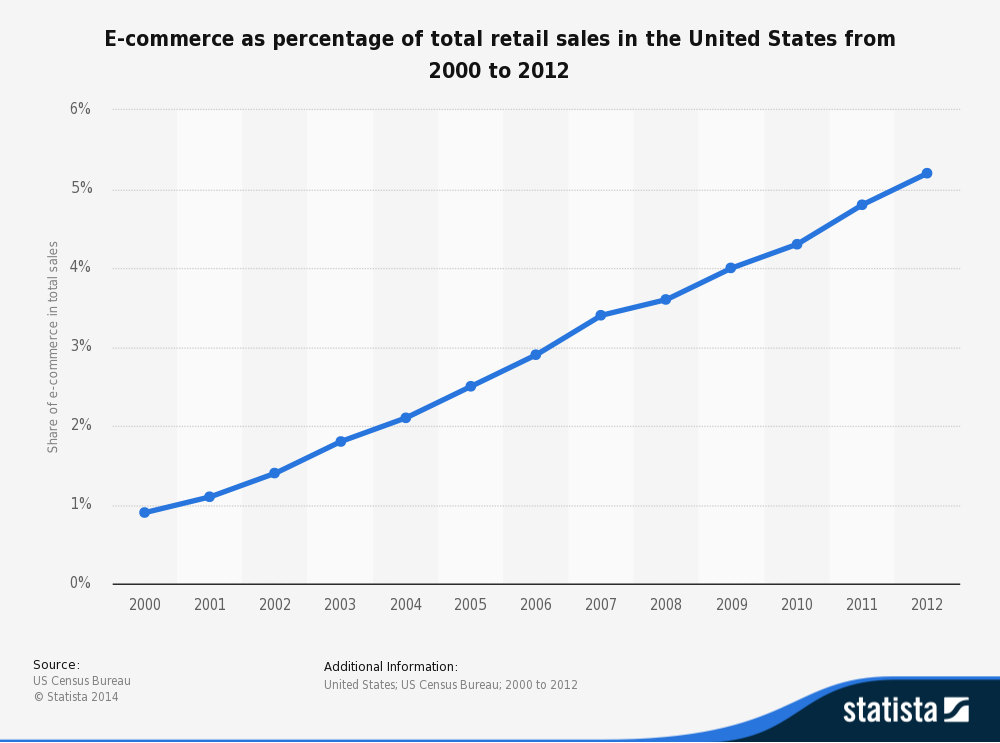
\includegraphics[width=0.7\textwidth]{figuras/ecommerce_percent.jpg}
	\caption{\ecommerce como porcentaje de las ventas totales en Estados Unidos}
	\label{figure:ecommerce_percent_sales}
\end{figure}

Acorde a toda información disponible, las ventas \ecommerce continuaron creciendo en los siguientes años y, en 2012 las ventas \ecommerce representaron el 5.2\% de las ventas totales en el mundo. Como se puede observar en \refFigura{figure:ecommerce_percent_sales}.

\ecommerce tiene muchas ventajas sobre tiendas \brickandmortar y catálogos de venta por correo. Los consumidores pueden fácilmente buscar a través de una base de datos muy extensa de productos y servicios. Pueden ver los precios reales, definir una orden de compra en varios días y enviar un correo como un \wishlist esperando que alguien pague por sus productos seleccionados. Los clientes pueden comparar precios con un simple \click del \mouse y comprar los productos seleccionados al mejor precio.

Proveedores \online, en sus turnos, también tienen claras ventajas. La \web y sus motores de búsqueda proveen una manera para encontrar clientes sin campañas de publicidad costosas. Incluso tiendas \online pequeñas pueden alcanzar mercados globales. 

La tecnología \web también permite realizar un seguimiento sobre las preferencias de los clientes para ofrecer una comercialización personalizada.

%La historia de \ecommerce is impensable sin Amazon e Ebay los cuales estuvieron entre las primeras compañías que permitían transacciones electrónicas. Gracias a sus fundadores ahora tenemos un sector considerable de \ecommerce y disfrutar de comprar y vender gracias a la Internet. Actualmente hay 5 de los mas grandes y mas famosos \textit{worldwide internet retailers}: Amazon, Dell, Staples, Office Depot y Hewlett Packard. De acuerdo a las estadísticas, las categorías de productos mas vendidos en \textit{Worl Wide Web} son música, libros, computadores, artículos de oficina y otros dispositivos electrónicos.
%
%Amazon.com, Inc. es uno de las mas famosas compañías \ecommerce  para vender productos sobre la Internet. Después del colapso \textit{dot-com} Amazon perdió su posición de modelo de negocio exitoso, sin embargo, en 2003 la compañía hizo su primer año con utilidades el cual fue el primer paso para el desarrollo futuro.
%
%Al principio Amazon.com fue considerado como una tienda \textit{online} de libros, pero con el tiempo una variedad de productos electrónicos fueron agregados, software, DVDs, juego de video, CDs de música, MP3s, prendas de vestir, calzado, productos de salud, etc. El nombre original de la compañía fue Cadabra.com, pero rápidamente después que se volviera popular Internet Bezos decidió cambiar el nombre de su negocio a “Amazon” después del río voluminoso mas grande del mundo. En 1999 Jeff Bezos fue nombrado como la persona del año por Time Magazine en reconocimiento al éxito de la compañía. Aunque la sede principal de la empresa se encuentra en USA, WA, Amazon ha establecido sitios \textit{web} separados en otros países tales como United Kingdom, Canada, France, Germany, Japan, y China. La compañía apoya y opera \textit{retail web sites} para muchos negocios famosos, incluyendo Marks \& Spencer, Lacoste, la NBA, Bebe Stores, Target, etc.
%
%Amazon es uno de los primeros negocios \ecommerce en establecer un programa de marketing para los afiliados, y actualmente la compañía obtiene cerca del 40\% de sus ventas desde afiliados y vendedores de terceras partes que lista y vende productos en el sitio \textit{web}. En 2008 Amazon penetro en el cine y actualmente esta patrocinando la película \textit{“The Stolen Child”} con \textit{20th Century Fox}.
%
%Acorde a las investigaciones en 2008, el dominio Amazon.com a traído cerca de 615 millones de clientes cada año. La característica mas popular del sitio \textit{web} es el \textit{review sistem}, i.e., la habilidad de los visitantes de presentar sus \textit{reviews} y \textit{rate} cualquier producto en un \textit{raiting scale} de uno a 5 estrellas. Amazon.com es también \textit{well-know} por su \textit{clear and user-friendly} avanzado sistema de búsqueda que permite a los visitantes buscar por \textit{keywords} en el texto completo de muchos libros en la base de datos.
%
%Otra compañía ha contribuido mucho en el proceso de desarrollo de \ecommerce es Dell Inc., una compañía americana posicionada en Texas, que se sitúa en el tercer lugar de ventas de computadoras después de Hewllett-Packard y Acer.
%
%Lanzado en 1994 como una pagina estática, Dell.com ha realizado rápidos pasos, y para finales de 1997 fue la primera compañía en lograr el \textit{record} de un millón de ventas \textit{online}. Su única estrategia de ventas sobre la \textit{World Wide Web} sin \textit{retail outlets} y sin intermediarios ha sido admirado por un sin fin de clientes e imitado por un gran numero de \ecommerce \textit{businesses}. El factor de éxito de Dell es que Dell.com permite a los clientes elegir y controlar, i.e., visitantes pueden explorar el sitio y ensamblar PC pieza por pieza eligiendo el mas mínimo componente basado en sus presupuestos y requerimientos. De acuerdo a las estadísticas, aproximadamente la mitad de las ganancias de las compañías proviene desde su sitio \textit{web}.
%
%En 2007, Fortune magazine \textit{ranked} Dell como la \textit{34th-largest} compañía en \textit{Fortune 500 list}, y \textit{8th} en su \textit{Top 20 list} anual de las mas exitosas y admiradas compañías en USA en reconocimiento al \textit{bussiness model} de la compañía.

La historia de \ecommerce es nueva, un mundo virtual que esta evolucionando de acuerdo a las ventajas del cliente. Es un mundo que todos construyen en conjunto ladrillo por ladrillo, estableciendo una base segura para las nuevas generaciones.

\subsection{\ecommerce en la actualidad}

En la actualidad, \ecommerce es una experiencia destacable. Transformo las compras tradicionales mas allá de lo reconocible. La experiencia es mucho mejor que cualquier otra manera de comprar, seduciendo a una gran cantidad de \ecommerce \lovers.

Si hace algunos años atrás \ecommerce fue una palabra de moda, ahora se ha convertido en la orden del día. Al parecer las personas compran literalmente en cualquier parte - en sus lugares de trabajo, durante el almuerzo, en las horas punta cuando no hay nada mas por hacer salvo encender el computador y comenzar a navegar.

En el presente, \ecommerce ha ganado tanta popularidad debido a que su tecnología subyacente esta evolucionando a pasos agigantados. Incluso se esta ofreciendo \textit{"sentir"} el producto con un \mouse \textit{3D} para comprender mejor su forma, tamaño y textura. ¿Para que salir cuando todo lo que se debe hacer es realizar un pedido, elegir la forma de envío, pararse y esperar hasta que la orden sea entregada hasta la puerta?

\ecommerce hoy ofrece tanto lujo que incluso las tiendas convencionales han encendido las alarmas. Aunque, cada uno esta de acuerdo que hay un gran camino para que \ecommerce reemplace las tiendas, la posibilidad existe que ocurra en el futuro. \ecommerce del cual somos actualmente testigos trae tanta aventura a nuestras vidas que es disfrutado por toda la comunidad \online.

En la actualidad \ecommerce tiene algunos inconvenientes; pero quien no se arriesga, no cruza el río. Muchos consumidores están dispuestos a aguantar estas desventajas, ya que confían en el mundo \online y desean que sea un mejor lugar.

\ecommerce en la actualidad refleja lo que hemos creado desde un inicio para el comercio electrónico \online. Fue creado por nosotros y pensado para nosotros.

\subsection{\ecommerce en el futuro}

Expertos predicen un futuro prometedor y glorioso para \ecommerce. En un presumible futuro \ecommerce se confirmara por si misma como una herramienta importante para las ventas. El éxito de \ecommerce se convertirá en una noción inseparable de la \web ya que \eshopping se esta volviendo cada vez mas y mas popular y natural. Al mismo tiempo la competitividad en el mundo de los servicios \ecommerce intensificará su crecimiento. Así la tendencia que  prevalecerá \ecommerce será el crecimiento de las ventas por \internet y la evolución.

Cada año el numero de ofertas de \ecommerce crece enormemente. El volumen de ventas de las tiendas \online  son mas que comparables con esos \brickandmortar. Y la tendencia va a continuar, porque hay mucha gente \textit{encarcelada} por las obligaciones laborales y de los hogares, mientras que \internet permite ahorrar mucho tiempo y dinero al permitir  elegir los productos a los mejores precios. Hoy en día el auge de las ventas por \internet es la base del magnífico futuro \ecommerce.

La tendencia \textit{cantidad a calidad} del \ecommerce se está convirtiendo cada vez más evidente, ya que \internet ha incluido el factor geográfico de la venta. Así que no importa más si su tienda se encuentra en New York, Londres o en una pequeña ciudad. Para sobrevivir, los comerciantes tendrán que adaptarse rápidamente a las nuevas condiciones. Para atraer a más clientes, los propietarios de las tiendas \online tendrán no solo que incrementar el número de servicios disponibles, ademas deberán poner más atención a elementos como \design atractivo, \userfriendliness, presentación atractiva; tendrán que oportunamente emplear tecnología moderna para que sus negocios sean parte del futuro del \ecommerce.

Claramente, aquellos que adquieren \estores antes, tienen mejores oportunidades  para el éxito y prosperidad, aunque un sitio \ecommerce por si mismo no garantiza nada. Solo una apropiada solución \ecommerce en combinación con \emarketing y \advertising pueden asegurar éxito.


\section{Motivación}\label{cap:intro:motivacion}
\section{casa}

Acá va la motivación...

\begin{itemize}
	\item \textbf{\shoppingcart}:
	
	\item \textbf{Reclamos ciudadanos}: Un sistema para realizar y gestionar reclamos que estén relacionado principalmente temas sociales con el fin de alertar a la brevedad a los organismos públicos responsables. Ejemplos de uso serian: Calles en mal estado, semáforos en mal estado, semáforos que no tengan un tiempo suficiente para cruzar, cruces peligrosos para peatones, aceras en mal estado, lugares de ruido excesivo, lugares de robos comunes, plazas en mal estado. La idea básica es crear una queja, y que los ciudadanos que consideren que dicha queja los representa, unirse a ella para lograr un volumen crítico para que las autoridades sean consientes del impacto que genera dicha queja.
	
	\item \textbf{Reservas horas medicas:} Un sistema para gestionar las horas medicas que muestre sugerencias de acuerdo a la distancia que se encuentran los especialistas desde la \textit{geo-posicion} del sistema que realiza la solicitud. 
	
	\item \textbf{Consultas de libros en una biblioteca:} Un sistema para consultar la disponibilidad, la cantidad, la posibilidad de reservarlo, e incluso cuando sera devuelto.
	\item \textbf{Catálogo de Moteles}: Un catálogo de moteles de acuerdo a la \textit{geo-posicion} pueden ser listados para determinar las mejores opciones disponibles. Adicionalmente se podría mostrar los horarios disponibles de las habitaciones, e incluso poder generar reservas y pagar la habitación. De esta manera se optimiza el tiempo de los clientes, y los recursos de los proveedores.
	
	\item \textbf{Catalogo de Medicamentos}: Un catalogo completo de los medicamentos oficialmente aceptados podrían ser listados para entregar información relevante de acuerdo a las dosis así como de efectos adversos, si es necesaria una receta, etc. Otra cosa interesante, es dar la opción de mostrar todos los remedios genéricos que existen en el mercado. El escenario ideal seria ademas mostrar el precio de estos, así como la distancia a las droguerías en donde el producto se encuentra disponible.
	
	\item \textbf{Reserva de horas en Registro Civil}: Al menos en Chile, realizar un tramite en el registro civil es sinónimo de una perdida de tiempo absurda solo para ser atendido. Si la reserva de hora puede ser realizada desde cualquier sitio, el sistema se volvería drásticamente mas eficiente.
	
	\item \textbf{Catalogo de Fiestas}: Un catalogo con las fiestas disponibles tanto a la brevedad posible, como en el futuro. Que muestre información relevante 
	
\end{itemize}

Todas estas situaciones tienen algo en común, y es que los usuarios desean consultar información para tomar una decisión. El sistema idealmente permite contrastar datos entre diferentes proveedores de servicios similares, así como de aportar con información clara y relevante, para que futuros usuarios puedan tomar una decisión aun mas informados.

Como se puede concluir, el modelo de negocio de estas situaciones es en su mayoría el mismo, solo cambiado la presentación para hacerlo \adhoc a la situación.

\section{Alcances y Objetivo General}\label{cap:intro:alcances}
Desarrollar un código base que permita desarrollar una familia aplicaciones. Dicha aplicación se utilizara para desarrollar 3 ejemplos a fin de demostrar su utilidad.

\section{Objetivos Específicos}\label{cap:intro:objetivos}
%Dentro de los objetivos específicos se encuentran:
\begin{itemize}
	\item Determinar viabilidad del proyecto.
	\item Determinar la tecnología mas adecuada para el desarrollo del proyecto
	\item Determinar la arquitectura adecuada para el desarrollo de software genérico
	\item Desarrollar un \ecommerce
	\item Objetivo 4
\end{itemize}

\section{Caracteristicas deseables}\label{cap:intro:alcance}

\begin{table}[h!]
    \tiny
   
\begin{tabular}{ |L{0.6\paperwidth}|L{0.1\paperwidth}|}
\hline
	\task &
	Tiempo
	
\\ \hline
	\textbf{ Agregar \itemcommerce}: Agregar un \itemcommerce a la tienda.&
	
\\ \hline
	\textbf{ Remover \itemcommerce}: Remover un \itemcommerce de la tienda.&
	
\\ \hline
	\textbf{ Agregar \itemcommerce}: &
	
\\ \hline
	\textbf{ Agregar \itemcommerce}: &
	
\\ \hline
	\textbf{ Agregar \itemcommerce}: &
	
\\ \hline
	\textbf{ Agregar \itemcommerce}: &
	
\\ \hline
	\textbf{ \textit{\dragdrop} manejo de variedad}: Organizar el orden de la variedad de \itemcommerce en la tienda con \textit{\dragdrop}.&
	%\textbf{ Drag \& Drop Variant Management:} Arrange order of product's variants in your shop with drag and drop.&
		
\\ \hline
	\textbf{ \dragdrop \merchandising}: Organizar el orden de los productos en la tienda con \textit{\dragdrop}.&
	%\textbf{ Drag \& Drop Merchandising:} Arrange order of products in your shop with drag and drop.&
		
\\ \hline
	\textbf{Independencia del \device}: optimizar la experiencia para todas las plataformas: \mobile, \tablet y \desktop \devices.
	%\textbf{ Device Agnostic:} Optimized experience for all mobile, tablet, and desktop devices.&
		
\\ \hline
	 \textbf{Edición del campo \inline}: Agregar y editar contenido de la tienda \clicking cualquier \textfield.&
	% \textbf{ Inline Field Editing:} Add and edit your shop's content by clicking any text field.&
		
\\ \hline
	\textbf{ \googleanalytics}: \outofthebox \googleanalytics \event \tracking.&
	%\textbf{ \googleanalytics}: Out of the box Google Analytics event tracking.&
		
\\ \hline
	\textbf{ Integración de \paypal}: Soportar la opción de utilizar \paypal \checkout.&
	%\textbf{ PayPal Integration:} Supports the ability to use PayPal checkout.&
		
\\ \hline
	\textbf{\realtime \itemupdates}: Cambios realizados a la tienda son instantáneamente observados por los compradores (sin refrescar la página).&
	%\textbf{ Real-time Reactive:} Changes made to your shop are instantly seen by your shoppers (without page reloads).&
		
\\ \hline
	\textbf{Clonar productos existentes}: Crear nuevos productos clonando cualquier producto existente.&
	%\textbf{ Clone Existing Products:} Create new products by cloning any existing products.&
		
\\ \hline
	\textbf{Múltiples imágenes por variante de producto}: Agregar múltiples imágenes por opción de producto.&
%	\textbf{ Multiple Images Per Product Variant:} Add multiple product images per product option.&
		
\\ \hline
	\textbf{ Recursive Tag Taxonomy:} Uses recursive tag taxonomy para categorizar.&	
	%\textbf{ Recursive Tag Taxonomy:} Uses recursive tag taxonomy for categorization.&
		
\\ \hline
	 \textbf{ Clone Product Variants:} Create new product variants by cloning any existing product variant.&
	
\\ \hline
	\textbf{ Fully Open Source:} Node.js and Meteor. Completely Open source. All day. Every day.&
	
\\ \hline
	\textbf{ Quantity per Variant:} Inventory support by product variant.&
	
\\ \hline
	\textbf{ Published or Hidden Status:} Ability to have products in a "draft" state before publishing.&
	
\\ \hline
	\textbf{ Detalle de productos}: permite detalle de productos en \keyvalue \listhighlevel .&
%	\textbf{ Product Details:} Supports additional product details in key/value list.&
	
\\ \hline
	\textbf{ SEO Hashtags:} Uses social media hashtags for product urls for simple SEO+social media \tracking.&
	
\\ \hline
	\textbf{ \onepage \checkout:} \checkout todo en \onepage.&
	%\textbf{ One Page \checkout:} Checkout all done on one page.&
	
\\ \hline
	\textbf{ \shop \analytics:} Integrar \tracking \framework para integrar cualquier \analytics \system.&
	%\textbf{ Shop Analytics:} Integrated tracking framework for integration to any analytics system&
	
\\ \hline
	\textbf{ \dockerio listo}: \build, \ship y \run en cualquier lugar.&
	%\textbf{ Docker.io Ready:} Build, Ship and Run anywhere.&
	
\\ \hline
	 \textbf{ Backorders:} Shoppers can purchase products even when quantity runs out.&
	
\\ \hline
	\textbf{ i18n and l10n:} Internationalization and localization to translate and localize all content for the world.&
	
\\ \hline
	\textbf{ Variant Management:} Easily manage product options (e.g. size/color) and related product photos.&
	
\\ \hline
	\textbf{ App Gallery:} Select from a gallery of apps to extend your shop by adding your favorite tools.&
	
\\ \hline
	\textbf{ Social Media Integration:} Integrated custom product social media messaging (FB, Twitter, Pinterest, Instagram).&
	
\\ \hline
	\textbf{ Custom Domains:} Use your own domain names.&
	
\\ \hline
	\textbf{ Flat Rate Tax Management:} Manage tax rules for your store.&
	
\\ \hline
	\textbf{ Additional Payment Methods:} Support for more payment methods (providers TBD).&
	
\\ \hline
	\textbf{ Global Shipping:} Ship your products around the globe (carriers TBD).&
	
\\ \hline
	\textbf{ User Management:} Invite users and grant permissions.&
	
\\ \hline
	\textbf{ Email Templates:} Manage email templates for your shop.&
	
\\ \hline
	\textbf{ Hero Manager:} Inline management for hero sections on your shop.&
	
\\ \hline
	\textbf{ Search:} Auto-suggest, keyword product search.&
	
\\ \hline
	\textbf{ Braintree Integration:} Braintree Integration.&
	
\\ \hline
	\textbf{ Stripe Integration:} Use Stripe for payments.&
	
\\ \hline
	\textbf{ Native Mobile Apps:} Build and deploy iOS, Android native Reaction apps.&
	
\\ \hline
	\textbf{ Multi-Currency Support:} Support for additional currencies beyond US Dollars.&
	
\\ \hline
	\textbf{ RTL Localization:} Right to left language support.&
	
\\ \hline
	\textbf{ Revision Control:} Revision control with rollback for all edits.&
	
\\ \hline
	\textbf{ History Logging:} Full insight to all actions performed.&
	
\\ \hline
	\textbf{ Cash on Delivery Payments:} Cash on delivery payment methods.&
	
\\ \hline
	\textbf{ API:} Support for both HTTP API and Meteor DDP.&
	
\\ \hline
	\textbf{ Product Inheritance:} Manage product pricing, promotions, visibility through parent-child-clone inheritance.&
	
\\ \hline
	\textbf{ Coupon Codes:} Coupon management and tracking for discounts.&
	
\\ \hline
	\textbf{ Returns and Refunds:} Track, manage, and analytics on returns and exchanges.&
	
\\ \hline
	\textbf{ Multi-Vendor:} Multiple vendors with review, publish, drop shipping.&
	
\\ \hline
	\textbf{ Flexible Tax Management:} Manage and customize tax rules.&
	
\\ \hline
	\textbf{ Subscription Products:} Subscription based product types.&
	
\\ \hline
	\textbf{ Order Entry and Editing:} Adminstrator addition and editing of orders.&
	
\\ \hline
	\textbf{ Embed Social Content:} Embed reviews, tweets, and other social content.&
	
\\ \hline
	\textbf{ Bitcoin Integration:} Ability to accept Bitcoin payments in your shop.&
	
\\ \hline
	\textbf{ Amazon Payments Integration:} Use Amazon for payments.&
	
\\ \hline
	\textbf{ Promotions:} Ability to manage and track promotions by channels, events, and more.&
	
\\ \hline
	\textbf{ Google Wallet Integration:} Use Google Wallet for payments.&
	
\\ \hline
	\textbf{ Shipwire Integration:} Ability to use Shipwire for order fulfillment.&
	
\\ \hline
	\textbf{ ShipStation Integration:} Ability to use ShipStation for order fulfillment.&
	
\\ \hline
	\textbf{ MailChimp Integration:} Use MailChimp to collect and manage emails.&
	
\\ \hline
	\textbf{ Actionable Analytics:} Data driven product presentation, and performance analysis.&
	
\\ \hline
	\textbf{ Hotkeys:} Establish shortcuts for regular tasks to quickly trigger a Reaction action.&
	
\\ \hline
	\textbf{ Theme Gallery:} Select from a gallery of themes to change the design and experience of your shop.&
	
\\ \hline
	\textbf{ Import from Squarespace:} Import your product catalog from Squarespace into Reaction.&
	
\\ \hline
	 \textbf{ Import from Shopify:} Import your product catalog from Shopify into Reaction.&
	
\\ \hline
	\textbf{ Import from Magento:} Import your product catalog from Magento into Reaction.&
	
\\ \hline
	\textbf{ Import from Spree Commerce:} Import your product catalog from Spree Commerce into Reaction.&
	
\\ \hline
	\textbf{ Import from Big Commerce:} Import your product catalog from Big Commerce into Reaction.&
	
\\ \hline
	&
	
\\ \hline
	&
				
\\ \hline
\end{tabular}
    \caption{ Carta gant}
    \label{tab:task_proyect}
\end{table}

%TODO remover este codigo inecesario
%\section{Estructura de la memoria}\label{cap:intro:estructura}
%La estructura utilizada en este documento para exponer el trabajo realizado es la siguiente:
%
%\begin{itemize}
%	\item \textbf{Capítulo \ref{cap:intro}. \nameref{cap:intro}:} Corresponde a la descripción del tema, la motivación de éste y los alcances y objetivos del trabajo realizado.
%	
%	\item \textbf{Capítulo \ref{cap:antecedentes}. \nameref{cap:antecedentes}:} Corresponde a la revisión bibliográfica o antecedentes. En este capítulo se explican los conceptos necesarios para la comprensión y contextualización del trabajo.
%	
%	\item \textbf{Capítulo \ref{cap:conclusiones}. \nameref{cap:conclusiones}:}	Se enumeran las conclusiones del trabajo realizado y se proponen trabajos a realizar en el futuro.
%\end{itemize}
%%%%%%%%%%%%%%%%%%%%%%
%								%
%	ESTADO DEL ARTE				%
%								%
%%%%%%%%%%%%%%%%%%%%%
\chapter{Estado del Arte}\label{cap:estadoArte}

%Por definición \textit{e-Commerce}: Transacción comercial electrónica, así como sobre Internet.
%
%Vender y realizar transacciones como estas se pueden hacer gracias a \textit{World Wide Web}, el cual es una convinación global de \textit{links}, información, paginas \textit{web} y \textit{e-Commerce websites}.
%
%Con el fin de considerar 

%TODO


\textit{Open-source e-Commerce shopping carts} ofrecen muchas ventajas para \textit{small businesses}. Soluciones \textit{Open-source} pueden ser desarrolladas para ajustarse a las necesidades del negociante. Ellos contienen una gran combinación de características a un mínimo costo. Y, aunque las opciones de soporte pueden ser mas limitadas que las propietarias o \textit{hosted platforms}, soluciones independientes \textit{open-source} generalmente tienen grandes comunidades de desarrolladores y socios para ayudar a los nuevos comerciantes.

Aquí hay una lista de 11 \textit{open-source e-Commerce solutions}. El \textit{core} de todas las aplicaciones es \textit{free}. Cada aplicación tiene extensiones \textit{free} y \textit{premium} y opciones de soporte para mejorar el desarrollo de la \textit{store}.

\newcommand{\nameOpenCart}{OpenCart }
\subsection{\nameOpenCart}

\begin{figure}[h!]
	\centering
	\includegraphics[width=0.5\textwidth]{figuras/cap1/openCartWebsite.jpg}
	\caption{\nameOpenCart \textit{website}\cite{online_OpenCartWebsite}.}
\end{figure}

\nameOpenCart es una aplicación \textit{open-source}, basada en PHP, es una solucion \textit{e-Commerce} para comerciantes \textit{online}. \nameOpenCart tiene una comunidad activa y leal para el apoyo de usuarios, así como una lista de socios comerciales para instalación y customizacion profesional. En \nameOpenCart existen mas de 20 medios de pago, y mas de 8 métodos de envío para la descarga por defecto, con cientos de métodos adicionales para el envío y el pago en su directorio de extensiones. \nameOpenCart también fue diseñado para un manejo sencillo de múltiples compras desde una interfaz de administración. Tiene mas de 2700 \textit{themes}.

\newcommand{\namePrestaShop}{PrestaShop }
\subsection{\namePrestaShop}

\begin{figure}[h!]
	\centering
	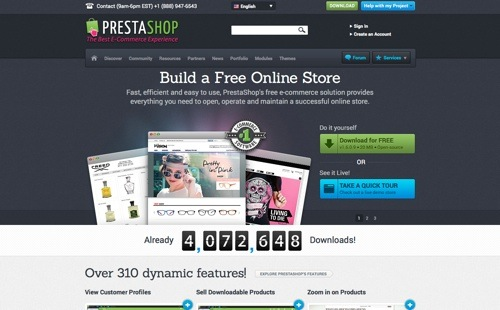
\includegraphics[width=0.5\textwidth]{figuras/cap1/PrestaShopWebsite.jpg}
	\caption{\namePrestaShop \textit{website}\cite{online_PrestaShop}.}
\end{figure}

\namePrestaShop es una solución \textit{e-Commerce} \textit{open-souce}, escrita en PHP y basada en \textit{Smarty template engine}. \namePrestaShop viene con mas de 310 características integradas y 3500 modulos y \textit{templates}. Cuenta con ventas cruzadas, productos descargables, la exportación de productos, una pagina de pago, envio, descuentos y mucho mas. Descargado mas de 4 millones de veces, \namePrestaShop es usado en 160 países y traducido a 63 idiomas. Tiene mas de 600000 miembros en su comunidad.

\newcommand{\nameMagento}{Magento }
\subsection{\nameMagento Community Edition}

\begin{figure}[h!]
	\centering
	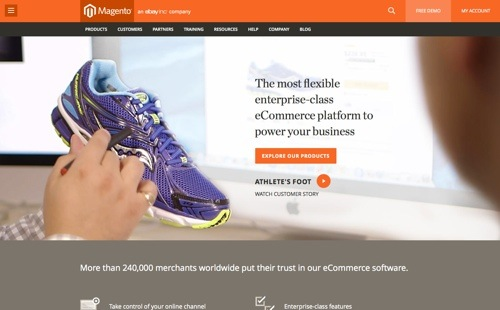
\includegraphics[width=0.5\textwidth]{figuras/cap1/MagentoWebsite.jpg}
	\caption{\nameMagento \textit{website}\cite{online_Magento}.}
\end{figure}

\nameMagento Community Edition es una version \textit{free} y \textit{open-source} de  una plataforma \textit{e-Commerce}. Los comerciantes pueden acceder a caracteristicas adicionales instalando las extensiones desde el gran \textit{\nameMagento Connect marketplace}. No existe soporte para \nameMagento Community Edition, así que las respuestas a las preguntas técnicas deben ser resultas a través del foro de usuarios. Un detalle, \nameMagento ha anunciado el cierro de su \textit{hosted solution}, \nameMagento Go, por ahora no habrían problemas con Community Edition. \nameMagento Community Edition soporta mas de 200000 sitios de clientes .

\newcommand{\nameZenCart}{Zen Cart }
\subsection{\nameZenCart}

\begin{figure}[h!]
	\centering
	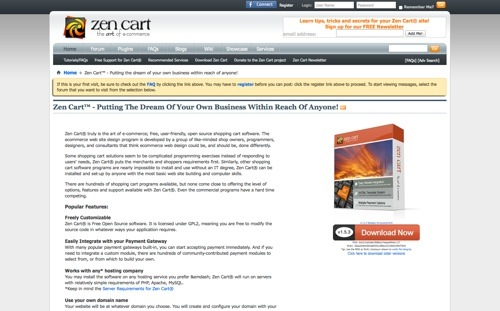
\includegraphics[width=0.5\textwidth]{figuras/cap1/ZenCartWebsite.jpg}
	\caption{\nameZenCart \textit{website}\cite{online_ZenCart}.}
\end{figure}

\nameZenCart es una aplicacion \textit{e-Commerce} \textit{open-source} escrita en PHP.\nameZenCart \textit{branched} desde el código osCommerce en 2003, con una solución que era mas \textit{template-based}. Tiene mas de 1800 \textit{add-ons} en 16 categorias. La comunidad de apoyo de \nameZenCart tiene aproximadamente 150000 miembros y 200000 \textit{threads}.

\newcommand{\nameSpreeCommerce}{Spree Commerce }
\subsection{\nameSpreeCommerce}

\begin{figure}[h!]
	\centering
	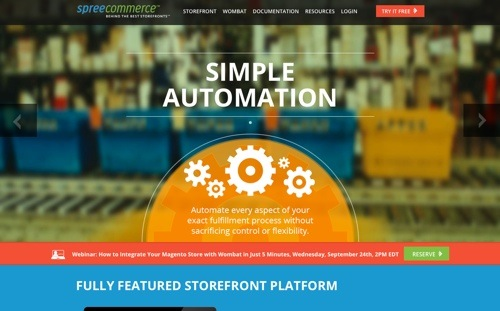
\includegraphics[width=0.5\textwidth]{figuras/cap1/SpreeCommerceWebsite.jpg}
	\caption{\nameSpreeCommerce \textit{website}\cite{online_SpreeCommerce}.}
\end{figure}

\nameSpreeCommerce es una solución \textit{e-Commerce} \textit{open-source}  basado en Ruby on Rails. La plataforma modular permite configurar, complementar, o reemplazar cualquier funcionalidad que necesites. \nameSpreeCommerce tiene mas de 45000 tiendas la plataforma al rededor del mundo, incluyendo Chipotle\cite{online_Chipotle} has more than 45,000 stores using the platform around the world, including Chipotle. Spree Commerce has been translated into more than 30 languages.

\newcommand{\nameDrupalCommerce}{Drupal Commerce }
\subsection{\nameDrupalCommerce}

\begin{figure}[h!]
	\centering
	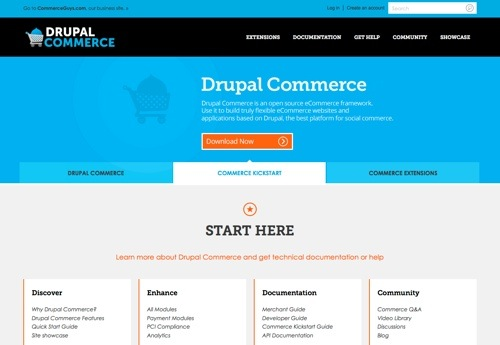
\includegraphics[width=0.5\textwidth]{figuras/cap1/DrupalCommerceWebsite.jpg}
	\caption{\nameDrupalCommerce \textit{website}\cite{online_DrupalCommerce}.}
\end{figure}	

\nameDrupalCommerce es una aplicación \textit{e-Commerce} desarrollado por  Commerce Guys. Construido sobre Drupal content management system. \nameDrupalCommerce ofrece un sistema de administración de producto completo, carro de compra varios lenguajes y monedas; y forma de pago. La lista de extension de \nameDrupalCommerce es una integración completamente en\textit{ third-party} para formas de pago,servicios de cumplimiento, aplicaciones de contabilidad, redes sociales y mucho mas. Paquetes de soporte técnico están disponibles por Commerce Guys.

\newcommand{\nameOsCommerce}{osCommerce }
\subsection{\nameOsCommerce}

\begin{figure}[h!]
	\centering
	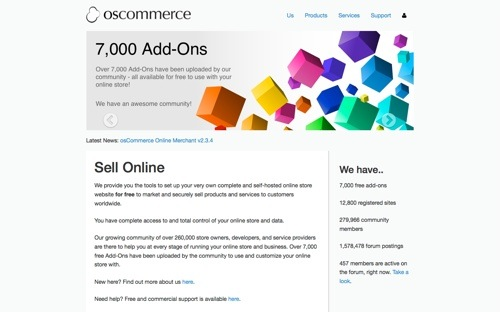
\includegraphics[width=0.5\textwidth]{figuras/cap1/osCommerceWebsite.jpg}
	\caption{\nameOsCommerce \textit{website}\cite{online_osCommerce}.}
\end{figure}

\nameOsCommerce (i.e., \textit{open source Commerce})es uno de las primeras aplicaciones \textit{e-Commerce} \textit{open-source}. Mas de 7000 \textit{free add-ons} han sido subidos por su comunidad para customizar una  \textit{online store}. \nameOsCommerce es usado por cerca de 13000 sitios registrados. La comunidad de apoyo tiene aproximadamente 280000 miembros los cuales han contribuido con 1.5 millones de posts en los foros. La comunidad directa juntos con miembros de otra comunidad están disponibles en vivo en el \textit{Chat room}.

\newcommand{\nameSimpleCart}{simpleCart }
\subsection{\nameSimpleCart}

\begin{figure}[h!]
	\centering
	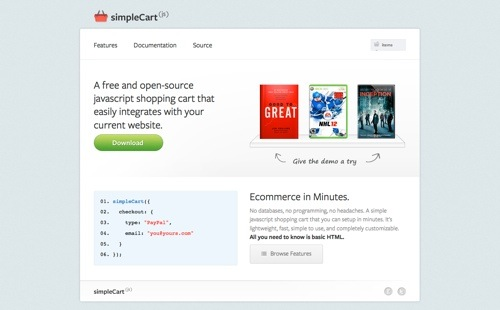
\includegraphics[width=0.5\textwidth]{figuras/cap1/simpleCartWebsite.jpg}
	\caption{\nameSimpleCart \textit{website}\cite{online_simpleCart}.}
\end{figure}

\nameSimpleCart(js) es un \textit{free} y \textit{open-source} JavaScript \textit{shopping cart}. Con su pequeño tamaño, \nameSimpleCart(js) esta disseñado para mantener simple  y sitions con alto trafico \textit{running fast}. \nameSimpleCart(js) tienen la habilidad de pagar con PayPal Express, Google Checkout, y Amazon Payments. \textit{Email checkout} e integracion con  Authorize.Net llegaran pronto.

\newcommand{\nameWooCommerce}{WooCommerce }
\subsection{\nameWooCommerce}

\begin{figure}[h!]
	\centering
	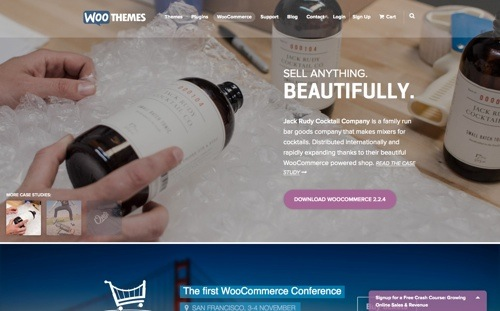
\includegraphics[width=0.5\textwidth]{figuras/cap1/WooCommerceWebsite.jpg}
	\caption{\nameWooCommerce \textit{website}\cite{online_WooCommerce}.}
\end{figure}

\nameWooCommerce es una aplicacion\textit{e-Commerce} \textit{free open-source} que permite a los comerciantes transformar \textit{WordPress sites} en \textit{stores}. \nameWooCommerce fue desarrollado por WooThemes desde un \textit{fork} de Jigoshop. \nameWooCommerce tiene una larga variedad de  \textit{plugins} y  \textit{themes} de WooThemes, como de sitios \textit{third party} tales como ThemeForest\cite{online_ThemeForest} y CodeCanyon\cite{online_CodeCanyon}. Con cerca de 4.5 millones de descargas desde \textit{WordPress.org}\cite{online_WordPress}, \nameWooCommerce es una solucion \textit{e-Commerce} muy popular para WordPress. Para obtener el soporte oficial de WooThemes, es necesario comprar un producto. De otra manera, obtener ayuda desde la comunidad activa del foro.

\newcommand{\nameWPECommerce}{WP e-Commerce }
\subsection{\nameWPECommerce}

\begin{figure}[h!]
	\centering
	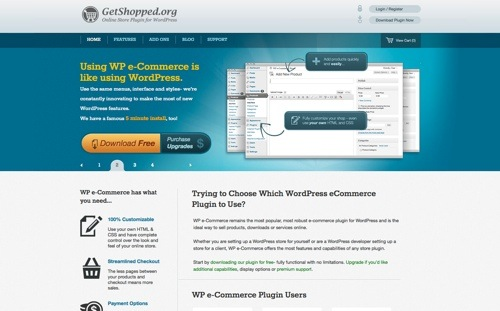
\includegraphics[width=0.5\textwidth]{figuras/cap1/WPECommerceWebsite.jpg}
	\caption{\nameWPECommerce \textit{website}\cite{online_WPECommerce}.}
\end{figure}

\nameWPECommerce es otra aplicacion popular obtenida desde la conversion del  sitio WordPress a una \textit{e-Commerce store}.\nameWPECommerce tiene cerca de 3 millones de descarga de \textit{plugin} desde \textit{WordPress.org}. Usa el propuo HTML y CSS y obten el control completo sobre la vista y la experiencia de tu \textit{online store}.\nameWPECommerce tiene una gran variedad de caracteristicas estandar, incluyendo \textit{ multi-tier pricing} para descuentos por cantidad e integración con redes sociales para \textit{marketing}. Para soporte, hay tutoriales en video y un foro en  \textit{ WordPress.org} ,tambien como consultantes de caracteristicas para ayuda profesional.

\newcommand{\nameJigoshop}{Jigoshop }
\subsection{\nameJigoshop}

\begin{figure}[h!]
	\centering
	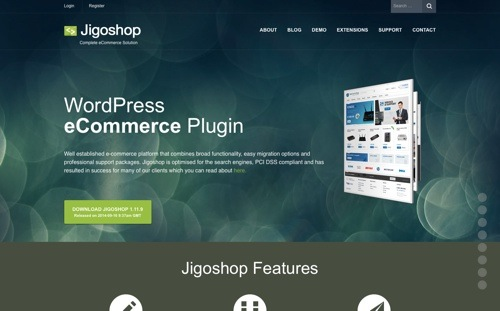
\includegraphics[width=0.5\textwidth]{figuras/cap1/JigoshopWebsite.jpg}
	\caption{\nameJigoshop \textit{website}\cite{online_Jigoshop}.}
\end{figure}

\nameJigoshop es una solucion \textit{e-Commerce} \textit{free} y \textit{open-source} basado en WordPress. Liberado en 2011, \nameJigoshop es el predecesor para WooCommerce. \nameJigoshop tiene mas de 30   \textit{themes}, 100 extensiones, y tres \textit{theme frameworks}. \nameJigoshop es  \textit{free}, asi como el soporte a \textit{WordPress.org}. Sin embago, el acceso a la comunidad de \textit{Jigoshop.com} comienza desde \$40 por mes.

\begin{table}[h!]
    \tiny
   
%\begin{tabular}{ |C{0.3\paperwidth}|C{0.3\paperwidth}| }
\begin{tabular}{ |l|c|c|c|c| }
\hline
	&
	traider\cite{online_Traider}&
	ReactionCommerce\cite{online_reactionCommerce}&
	NodeShop\cite{online_NodeShop}&
	Forward\cite{online_Forward}
 
\\ \hline
	Tecnología &
	bootstrap, nodejs and mongodb &
	Nodejs, Meteor, Mongodb, CoffeScript, Bootstrap, Docker&
	&
	

\\ \hline
	Mobile &
	&
	&
	&
\\ \hline
	version &
	&
	&
	0.06 ( 21/08/2013 )&
	0.1

\\ \hline
\end{tabular}
    \caption{ Resumen tecnologías entre diferentes opciones \textit{e-Commerce}}
    \label{tab:resume_technology_ecommerce}
\end{table}

Como se observa, existe una gran cantidad de aplicaciones \textit{open-souce} las cuales están disponibles para ingresar al mundo del comercio electrónico. Todas estas opciones tienen grandes comunidades que las respaldan, así como muchos usuarios satisfechos. 

Considerando esto, ¿ habrá alguna razón que justifique el desarrollo de un proyecto de estas características?

\section{Justificación para el desarrollo del proyecto}\label{cap:estadoArte:justificacion_proyecto}

\subsection{Nueva tecnología no es sinónimo de mejores soluciones}
%TODO
\subsubsection{El contexto como variable para la mejor solución}
%TODO


Node no es la panacea para todo, tiene muchos issues con los cuales hay que lidiar, pero es probable una de las mejores soluciones que se pueden tomar(LinkedIn).

***************************************************************************
Kiran Prasad, Sr. Director, Mobile Engineering, LinkedIn

Una pregunta interesante saber cuales son los problemas que te hicieron mirar hacia nodeJ(pregunta a KIRAN Prased)

Cuando llegue a LinkedIN estabamos corriendo cosas en Ruby and Rails stack, una de las cosas que encontramos es que el FRONT-END 

eficiencia en memoria



***************************************************************************
Sri Viswanath, SVP Engineering and Operations, Groupon

low latency


***************************************************************************
Jigar Desai, Sr. Director, Platforms, eBay

***************************************************************************
Billy Scott, PayPal

\subsubsection{Node.js vs Java \cite{online_nodejs_paypal}}


La primera adopción que hizo Paypal con Node.js no fue una aplicación menor; esto fue su \textit{account overview page} y una de las mas \textit{trafficked} \textit{apps} en el \textit{website}. Ellos tomaron un gran riesgo, pero lo hicieron con la finalidad de determinar si realmente la nueva plataforma representaba una mejora con respecto al sistema actual.
%Our first adopter of node.js in production wasn’t a minor application; it was our account overview page and one of the most trafficked apps on the website. We decided to go big, but we also mitigated that risk by building the equivalent Java application in parallel. We knew how to deploy and scale Java applications, so if anything went wrong with the node.js app, we could fall back to the Java one. This provided the setting for some interesting data.

Una vez que la aplicación con Node.js logro las mismas funcionalidades que la aplicación actual, persivieron el siguiente resultado:

\begin{itemize}
\item Fue construida casi \textbf{el doble de rapido con menos personal}.
\item Escrito con un \textbf{33\% menos de lineas de código}.
\item Construida con \textbf{40\% menos de archivos}.
\end{itemize}

Por si solo, esto mostro evidencia que mostraba a los equipos desarrollar más rápido utilizando \textit{JavaScript}

Performance fue un tópico interesante. Se pudo analizar 2 aplicaciones con exactamente las mismas funcionalidades: una con \textit{framework} Java interno basado en Spring y la otra construida en \textit{kraken.js} usando \textit{express}, \textit{dust.js} y otros códigos \textit{open source}.
%Performance is a fun and debatable topic. In our case, we had two applications with the exact same functionality and built by roughly the same teams: one on our internal Java framework based on Spring and the other built on kraken.js using express, dust.js and other open source code.

Se ejecutaron los test adecuados utilizando \textit{hardware} de producción que probaran las rutas y recolectaran \textit{data} rendimiento y tiempo de respuesta.
%We ran our test suite using production hardware that tested the routes and collected data on throughput and response time.

\begin{figure}[h!]
	\centering
	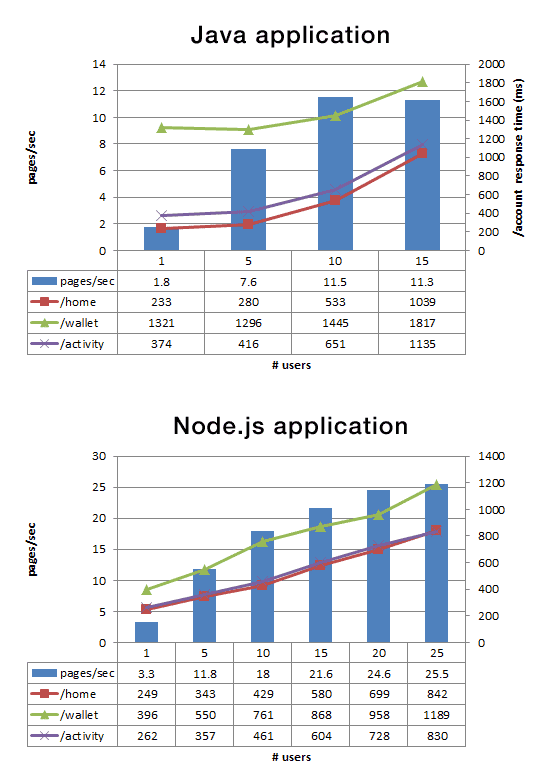
\includegraphics[width=0.6\textwidth]{figuras/cap2/java_nodejs_benchmark_paypal.png}
	\caption{\textit{Performance} de la aplicación en Java y Node.js}
	\label{cap2:figure:java_benchmark_paypal}
\end{figure}

Se observa que la aplicación que utiliza Node.js tiene:
%You can see that the node.js application had:



\begin{itemize}
\item El doble de solicitudes por segundo vs. la aplicación Java. Esto es incluso mas interesante porque los resultados iniciales de rendimiento estaban utilizando un solo nucleo para la aplicación Node.js, en comptaración con cinco nñucleos en Java. Se espere aumentar aun más esta brecha en el futuro.
%Double the requests per second vs. the Java application. This is even more interesting because our initial performance results were using a single core for the node.js application compared to five cores in Java. We expect to increase this divide further.
\item \textbf{Disminución en un 35\% en el tiempo promedio de respuesta} para la misma página. Esto se resulto ser \textbf{200ms mas rápido} en el servidor. Algo que los usuarios definitivamente notan.
%35% decrease in the average response time for the same page. This resulted in the pages being served 200ms faster— something users will definitely notice.
\end{itemize}


%There’s a disclaimer attached to this data: this is with our frameworks and two of our applications. It’s just about as apples-to-apples a performance test as we could get between technologies, but your milage may vary. That said, we’re excited by what we’ve seen from node.js’ raw performance.

Mas ejemplos de benchmark \cite{online_nodejs_java_dzone}


\subsubsection{Node.js vs PHP\cite{online_nodejs_php_loadimpact}}

No es justo comprar Node.js con PHP. Lo que realmente se compara es Node.js y PHP+Apacha2 ( u otro servidor http ). Es este caso particular, las pruebas fueron realizadas usando Apache2 y \textit{mod_php}, dado que es por lejos la configuración mas común. 
%So no, it’s not fair to say that we compare Node.js and PHP. What we really compare is Node.js and PHP+Apache2 (or any other http server). For this article, I’ve used Apache2 and mod_php since it’s by far the most common configuration. Some might say that I’d get much better results if I had used Nginx or Lighthttpd as the http server for PHP. That’s most likely very true, but at the end of the day, server side PHP depends on running in multiple separate processes. Regardless if we create those processes with mod_php or fastcgi or any other mechanism. So, I’m sticking with the standard server setup for PHP and I think that makes good sense.





\begin{figure}[h!]
	\centering
	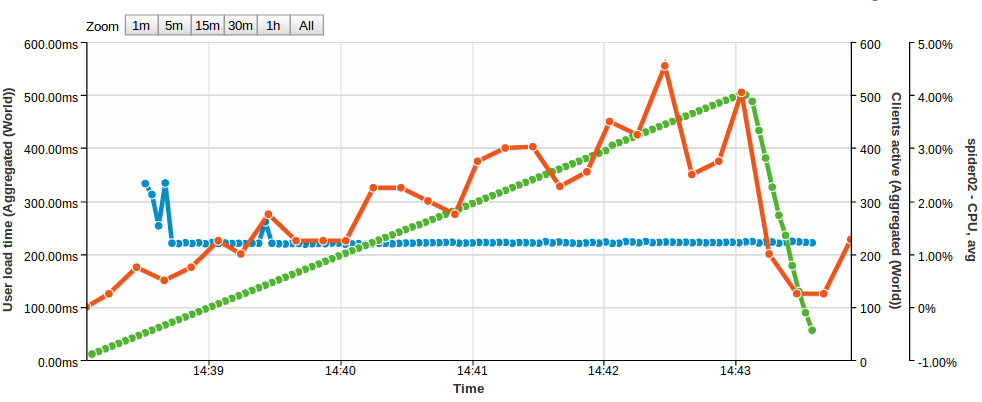
\includegraphics[width=0.6\textwidth]{figuras/cap2/node_benchmak_loadimpact.png}
	\caption{\textit{Performance} de la aplicación Node.js}
	\label{cap2:figure:java_benchmark_paypal}
\end{figure}

El primer grafico muetra lo que sucede cuando se carga el test en el servidor utilizando Node.js. La respuesta de tiempo (azul) es mucho mas constante durante todo el test. 

%The first graph here shows what happens when we load test the Node.js server. The response time (blue) is pretty much constant all through the test. My back of a napkin analysis of the initial outliers is that they have to do with a cold MySQL cache. Now, have a look at the results from the PHP test:


\begin{figure}[h!]
	\centering
	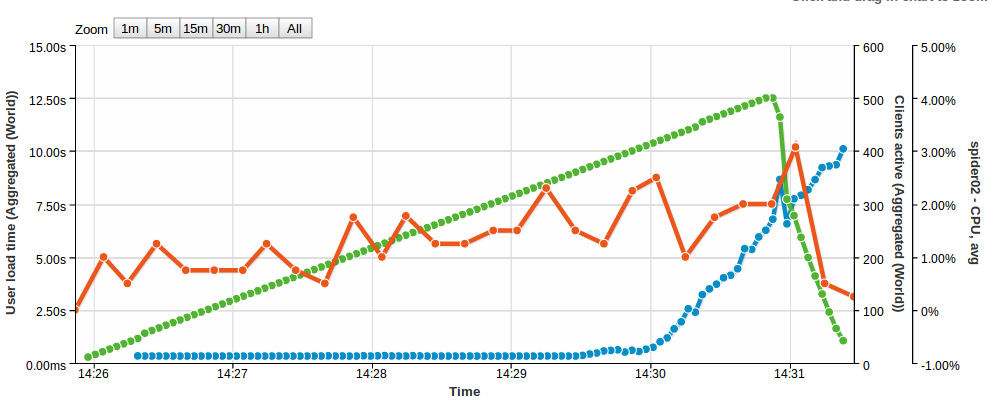
\includegraphics[width=0.6\textwidth]{figuras/cap2/phpapache_benchmak_loadimpact.png}
	\caption{\textit{Performance} de la aplicación en PHP/Apache}
	\label{cap2:figure:java_benchmark_paypal}
\end{figure}

Muy diferente los resultados para el caso de PHP. No es sencillo observar que sucede, pero las lineas azules están inicialmente estables a 320ms hasta cerca de 340 usuarios activos simultáneos. Después de eso, se observa un pequeño incremento en el tiempo de respuesta pero después de agregar mas usuarios activos simultáneos, el tiempo de respuesta se dispara por completo. 
%Quite different results. It’s not easy to see on this screen shot, but the blue lines is initially stable at 320 ms response time up to about 340 active concurrent users. After that, we first see a small increase in response time but after additional active concurrent users are added, the response time eventually goes through the roof completely.

¿ Qué problema tiene PHP/Apache?
%So what’s wrong with PHP/Apache?

La diferencia no es de sorprender. Esto es producto de la diferencia de arquitectura entre ambas soluciones.
%Ok, so what we’re looking at is not very surprising, it’s the difference in architecture between the two solutions. Let’s think about what goes on in each case.

Cuando Apache2 sirve a una pagina PHP, este deja la ejecución PHP a un \textit{child process} específico. Ese \textit{child process} puede solo manejar una solicitud PHP al mismo tiempo, así que si hay mas solicitudes, las otras deben esperar. En el servidor hay un máximo de 256 clientes (MaxClients) configurados vs 150 que vienen por defecto. Incluso si es posible aumentar el MaxClients hasta mas allá de 256, habrá problemas con la memoria interna(RAM), Al final, se necesita encontrar el balance correcto entre el máximo numero de solicitudes simultaneas y los recursos disponibles del servidor.
%When Apache2 serves up the PHP page it leaves the PHP execution to a specific child process. That child process can only handle one PHP request at a time so if there are more requests than than, the others have to wait. On this server, there’s a maximum of 256 clients (MaxClients) configured vs 150 that comes standard. Even if it’s possible to increase MaxClients to well beyond 256, that will in turn give you a problem with internal memory (RAM). At the end, you need to find the correct balance between max nr of concurrent requests and available server resources.

Pero para Node.js, es sencillo. Después de todo, cada solicitud es cerca de 30\% mas rápido que PHP, así que en \textit{performance}, el cual es una configuración extremadamente básica, Node.js es mas rápido. Ademas, en Node.js Todo esta en un solo proceso en el servidor. Un proceso manejando una solicitud activa. Así que no existe una comunicación interna de procesos entre diferentes instancias y el proceso madre. Incluso, pos solicitud, Node es mucho mas eficiente. PHP/Apache necesita muchísimo PHP y sobrecarga de procesos por cada simultaneo  \textit{worker/client}mientras Node compartirá la mayoría de su memoria entre las solicitudes.
%But for Node, it’s easier. First of all, in the calm territory, each request is about 30% faster than for PHP, so in pure performance in this extremely basic setup, Node is quicker. Also going for Node is the fact that everything is in one single process on the server. One process with one active request handling thread. So thre’s no inter process communication between different instances and the ‘mother’ process. Also, per request, Node is much more memory efficient. PHP/Apache needs to have a lot of php and process overhead per concurrent worker/client while Node will share most of it’s memory between the requests.

%Also note that in both these tests, CPU load was never a problem. Even if CPU loads varies with concurrent users in both tests it stays below 5% (and yes, I did not just rely on the graph, I checked it on the server as well). (I’ll write a follow up on this article at some point when I can include server memory usage as well). So we haven’t loaded this server into oblivion in any way, we’ve just loaded it hard enough for the PHP/Aapache architecture to start showing some of it’s problems.

Mas ejemplos de \textit{benchmark} \cite{online_nodejs_java_appdynamics}


\subsubsection{¿ Qué hace a Node.js mejor?}

Node.js introduce al menos 2 nuevas características ( para una amplia audiencia ). Primero, la habilidad  de escribir código JavaScript en el lado del servidor. En teoría esto puede ser una ventaja dado que JavaScipt es mas importante que nunca en el lado del cliente y usando el mismo lenguaje en el servidor y en el navegador deberían haber muchísimos beneficios. 
%Node.js introduces at least two new things (for a broader audience). First, the ability to write server side JavaScript code. In theory this could be an advantage since JavaScript is more important than ever on the client side and using the same language on server and browser would have many benefits. That’s at least quite cool.

La otra cosa que introduce Node.js es que es completamente asíncrono y orientado al evento. Node.js esta basado en el supuesto que muchísimo código de computador realmente espera por I/O la mayoría del tiempo, como esperando por un archivo para ser escrito en el disco o por una solicitud MySQL para retornar \textit{data}. Para lograr eso, mas o menos cada función en Node.js es \textit{non-blocking}.
%The other thing that makes Node.js different is that it’s completely asynchronous and event driven. Node is based on the realization that a lot of computer code actually just sits idle and wait for I/O most of the time, like waiting for a file to be written to disk or for a MySQL query to return data. To accomplish that, more or less every single function in Node.js is non-blocking.

Cuando se solicita a nodo abrir un archivo, no se espera a que retorne. En lugar de eso, se le comunica a Node.js a que función se le entrega el resultado y continuar con otra ejecución. Esto conduce a una dramática diferencia  para estructurar el código con \textit{callback} anidados y funciones anónimas de clausura.  Terminaras con algo como esto:
%When you ask for node to open a file, you don’t wait for it to return. Instead, you tell node what function to pass the results to and get on with executing other statements. This leads to a dramatically different way to structure your code with deeply nested callbacks and anonymous function and closures. You end up with something  like this:


\medskip
\begin{lstlisting}[caption= Ejemplo de anidación de funciones.]
	doSomething(val, function(err,result){
		doSomethingElse(result,function(err,res){
			doAbra();
			doKadabra(err, res, function() {
				...
				...
			});
		});
	});
\end{lstlisting}


La cualidad que hace diferente a Node.js, es que no es necesario utilizar un servidor http(s) separado. Es completamente común poner Node.js detrás de un Nginx, pero eso no es estrictamente necesario. Así que el corazón de las aplicaciones \textit{web} típicas de Node.js  es la implementación de su servidor real.
%It’s quite easy to end up with very deep nesting that in my opinion sometimes affects code readability in a negative way. But compared to what gets said about PHP, that’s very mild critique. And.. oh! The third thing that is quite different is that in Node.js, you don’t have to use a separate http(s) server. It’s quite common to put Node.js behind a Nginx, but that’s not strictly needed. So the heart of a typical Node.js web application is the implementation of the actual web server.


*****************************************************************************


Hopefully, this shows the inherit differences in two different server technologies. One old trusted and one young and trending. Hopefully it’s apparent that your core technical choices will affect your server performance and in the end, how much load you can take. Designing for high load and high scalability begins early in the process, before the first line of code is ever written.

And sure, in real life, there are numerous of tricks available to reduce the effects seen here. In real life, lots of Facebook still runs on PHP.


\subsection{Base de datos}

%TODO inicio de antiguo base de datos

base de datos escablaves horizontalmente, SQL escalables verticalmente.




What about transactions?


Many people bring up MongoDB’s lack of atomic transactions across collections as evidence that it’s not suitable for e-commerce applications. This has not been a significant barrier in our experience so far.

There are other ways to approach data integrity. In systems with low-moderate data contention, optimistic locking is sufficient. We’ll share more details about these strategies as things progress.



\begin{table}[h!]
    \tiny
   
%\begin{tabular}{ |C{0.3\paperwidth}|C{0.3\paperwidth}| }
\begin{tabular}{ |l|c|c|c|c|c| }


\hline
	&
	\textit{Free database backend support}&
	Language&
	\textit{\gloss{waf}}&
	License&

\\ \hline
	\nameOpenCart &
	MySQL&
	PHP&
	&
	GPLv3&
	
\\ \hline
	\namePrestaShop &
	MySQL&
	PHP&
	&
	Open Software License&
	
\\ \hline
	\nameMagento &
	MySQL&
	PHP&
	Zend Framework\cite{online_zend_framework}&
	Open Software License&
	
\\ \hline
	\nameZenCart &
	&
	&
	&
	&
 
\\ \hline
	\nameSpreeCommerce &
	MySQL, PostgreSQL, SQLite3&
	Ruby\cite{online_ruby_language}&
	Ruby on Rails\cite{online_ruby_rails}&
	New BSD License&

\\ \hline
	\nameDrupalCommerce &
	MySQL, PostgreSQL, SQLite3&
	PHP&
	Drupal\cite{online_drupal}&
	GNU GPL&
	
\\ \hline
	\nameOsCommerce &
	&
	&
	&
	&

\\ \hline
	\nameSimpleCart &
	&
	&
	&
	&
	
\\ \hline
	\nameWooCommerce &
	MySQL&
	PHP&
	WordPress\cite{online_wordpress}&
	GNU GPL&
	
\\ \hline
	\nameWPECommerce &
	&
	&
	&
	&
	
\\ \hline
	\nameJigoshop &
	MySQL&
	PHP&
	WordPress\cite{online_wordpress}&
	GNU GPL&
	
\\ \hline
\end{tabular}
    \caption{ Comparación entre diferentes opciones \textit{e-Commerce}}
    \label{tab:wide_table}
\end{table}


%TODO fin de antiguo base de datos


\subsection{Base de datos}

\textit{Relational databases} se encuentran en la mayoria de las organización desde hace muchisimo tiempo, y por buenas razones. \textit{Relational databases} apoya las aplicaciones del pasado que cumplen con las necesidades de negocio actuales; Estas son apoyadas por un extenso ecosistema herramientas; y hay una gran cantidad de mano de obra calificada para implementar y mantener estos sistemas.
%Relational databases have a long-standing position in most
%organizations, and for good reason. Relational databases
%underpin legacy applications that meet current business
%needs; they are supported by an extensive ecosystem of
%tools; and there is a large pool of labor qualified to
%implement and maintain these systems.

Pero las compañías están cada vez mas considerando la opción de alternativas para la infraestructura relacional heredada. En algunos casos la motivación es técnica, tal como la necesidad de escalar o actuar mas allá de las capacidades de sus sistemas actuales. Mientras que en otros casos, las compañías están motivadas por el deseo de identificar alternativas viables a \textit{softwares} propietario de alto costo. una tercera motivación es la agilidad y velocidad del desarrollo, dado que las compañías ansían adaptarse al mercado mas rápido y adoptar metodologías de desarrollo ágil.
%But companies are increasingly considering alternatives to
%legacy relational infrastructure. In some cases the
%motivation is technical — such as a need to scale or
%perform beyond the capabilities of their existing systems —
%while in other cases companies are driven by the desire to
%identify viable alternatives to expensive proprietary
%software. A third motivation is agility or speed of
%development, as companies look to adapt to the market
%more quickly and embrace agile development
%methodologies.

Estas opciones se aplican tanto para aplicaciones analíticas como transaccionales. Las compañías están cambiando \textit{workloads to Hadoop} para sus \textit{offline}, \textit{analytical workloads}, y están construyendo \textit{online}, aplicaciones operaciones con una nueva clase de tecnología de manejo de datos llamada "\gloss{nosql}", como por ejemplo \textit{MongoDB}
%These drivers apply both to analytical and transactional
%applications. Companies are shifting workloads to Hadoop
%for their offline, analytical workloads, and they are building
%online, operational applications with a new class of data
%management technologies called "NoSQL", or "Not Only
%SQL", such as MongoDB

\subsubsection{\gloss{sql} and the Relational Model}

\gloss{sql} es un lenguaje declarativo de consulta de datos . Un lenguaje declarativo es uno en el cual un programador especifica lo que desea y el sistema lo ejecuta, en lugar de definir proceduralmente como el sistema debería hacerlo. Unos pocos ejemplos incluyen: encontrar el registro del empleado 39, mostrar solo el nombre y el numero de teléfono del empleado de la totalidad de su registro, filtrar los registros de los empleados a aquellos que trabajan en contabilidad, contar la cantidad de empleados en cada departamento, unir la información de la tabla de los empleados \textit{employees} con la tabla de \textit{managers}.
%SQL is a declarative language for querying data. A declarative language is one in which a programmer specifies what they want the system to do, rather than procedurally defining how the system should do it. A few examples include: find the record for employee 39, project out only the employee name and phone number from their entire record, filter employee records to those that work in accounting, count the employees in each department, or join the data from the employees table with the managers table.


En una primera aproximación, \gloss{sql} permite consultar sobre aquellas preguntas sin pensar sobre como la información es expuesta en el disco, cuales indices utilizar para acceder a la información o que algoritmo utilizar para procesar la información. Un componente arquitectural significativo para la mayoría de los \textit{relational databases is a query optimizer}, el cual decide cual de las muchos equivalentes lógicos planea ejecutar las respuesta mas rápida a una \textit{query}. Estos optimizadores son usualmente mejores que los promedios de los usuarios de la \textit{database}, pero en algunas ocasiones ellos no tienen la suficiente información o tienen un modelo muy simple del sistema en \textit{order} para generar ejecuciones mas eficientes.
%To a first approximation, SQL allows you to ask these questions without thinking about how the data is laid out on disk, which indices to use to access the data, or what algorithms to use to process the data. A significant architectural component of most relational databases is a query optimizer, which decides which of the many logically equivalent query plans to execute to most quickly answer a query. These optimizers are often better than the average database user, but sometimes they do not have enough information or have too simple a model of the system in order to generate the most efficient execution.

\textit{Relational databases}, las \textit{databases} mas utilizadas en la practica, siguen el modelo de datos relacional. En este modelo, diferentes entidades del \textit{real-world} son guardadas en diferentes tablas. Por ejemplo, todos los \textit{employees} podrían ser guardados en una tabla \textit{Employees}, y todos los \textit{departments} podrían ser almacenados en la tabla \textit{Departments}.Cada fila de una tabla tiene varias propiedades guardadas en columnas. Por ejemplo, \textit{employees} podrían tener un \textit{employee id}, \textit{salary}, \textit{birth date}, y \textit{first/last names}. Cada una de estas propiedades sera guardada en una columna de la tabla \textit{Employees}
%Relational databases, which are the most common databases used in practice, follow the relational data model. In this model, different real-world entities are stored in different tables. For example, all employees might be stored in an Employees table, and all departments might be stored in a Departments table. Each row of a table has various properties stored in columns. For example, employees might have an employee id, salary, birth date, and first/last names. Each of these properties will be stored in a column of the Employees table.


El modelo relacional, va mano a mano con \gloss{sql}. \textit{Queries} simples de \gloss{sql}, tales como filtrar, recuperar todos los registros el cual sus campos hagan \textit{match} en algunos test( ejemplo, \textit{employeeid} = 3, o salary \> \$ 20000). Constructres mas complejos causan que \textit{database} haga trabajo extra, tal como \textit{joining} información sobre múltiples tablas (ejemplo., ¿ Cuál es el nombre del departamento en donde \textit{employee} 3 trabaja?). Otras estructuras complejas tal como \textit{aggregates} (ejemplo, ¿ cuál es el salario promedio de mis empleados?) puede manejar para \textit{full-table scans}.
%The relational model goes hand-in-hand with SQL. Simple SQL queries, such as filters, retrieve all records whose field matches some test (e.g., employeeid
% = 3, or salary \> \$ 20000). More complex constructs cause the database to do some extra work, such as joining data from multiple tables (e.g., what is the name of the department in which employee 3 works?). Other complex constructs such as aggregates (e.g., what is the average salary of my employees?) can lead to full-table scans.


\textit{Relational data model} define entidades altamente estructuradas con relaciones estrictas entre ellos. \textit{Quetying} este modelo con \gloss{sql} permite \textit{complex data transversa} sin desarrollar mucho. La complejidad del modelo y \textit{quering}, tienen sus limites, aunque:
%The relational data model defines highly structured entities with strict relationships between them. Querying this model with SQL allows complex data traversals without too much custom development. The complexity of such modeling and querying has its limits, though:

\textit{Complexity} guia a \textit{unpredictability}. La expresivilidad en \gloss{sql} implica un desafío en relación al costo de cada \textit{query}, y así el costo de \textit{workload}. Mientras, lenguajes de \textit{query} simples pueden complicar la lógica, al mismo tiempo hacen que sea sencillo proveer de almacenamiento de datos., cuando solo responde a \textit{requests} simples.
%Complexity leads to unpredictability. SQL's expressiveness makes it challenging to reason about the cost of each query, and thus the cost of a workload. While simpler query languages might complicate application logic, they make it easier to provision data storage systems, which only respond to simple requests.

Hay muchas maneras modelar un problema. \textit{Relational data model} es estricto: El \textit{schema} asignado para cada tabla especificada la \textit{data} en cada fila. Si se esta almacenando menos \textit{data} estructurada, o filas con mas diferencia en las columnas que se guardan, \textit{relational model} puede ser innecesariamente restrictiva. Similarmente, aplicaciones desarrolladas podrían no encontrar el \textit{relational model} idóneo para modelar cada tipo de \textit{data}. Por ejemplo, una gran cantidad den aplicaciones lógicas son escritas en lenguaje \textit{object-oriented} e incluye conceptos \textit{high-level} tales como \textit{lists}, \textit{queues}, y \textit{sets}, y algunos programadores desearan \textit{persistence layer} para modelar esto.
%There are many ways to model a problem. The relational data model is strict: the schema assigned to each table specifies the data in each row. If we are storing less structured data, or rows with more variance in the columns they store, the relational model may be needlessly restrictive. Similarly, application developers might not find the relational model perfect for modeling every kind of data. For example, a lot of application logic is written in object-oriented languages and includes high-level concepts such as lists, queues, and sets, and some programmers would like their persistence layer to model this.

Si la \textit{data} crece mas allá de la capacidad de un servidor, entonces las tablas en la \textit{database} tendrá que ser particionado a través de varios computadores. Para evitar \textit{JOINs} a través de la red para obtener todas las tablas requeridas, será necesario desnormalizarla. Desnormalizar guarda toda la \textit{data} de diferentes tablas que se desea observar en el mismo lugar. Esto hace que la \textit{database} simule una \textit{key-lookup store system}, dejando preguntas sobre la posibilidad de adaptarse mejor a la \textit{data}.
%If the data grows past the capacity of one server, then the tables in the database will have to be partitioned across computers. To avoid JOINs having to cross the network in order to get data in different tables, we will have to denormalize it. Denormalization stores all of the data from different tables that one might want to look up at once in a single place. This makes our database look like a key-lookup storage system, leaving us wondering what other data models might better suit the data.

Generalmente no es inteligente descartar años de consideraciones de diseño arbitrariamente.Cuando se considera el almacenamiento de la \textit{data} en una \textit{database}, considera \gloss{sql} y \textit{relational model}, los cuales son respaldados por décadas  de investigación y desarrollo, ofreciendo enriquecidas capacidades de modelamiento, y proveer garantías \textit{fácil-de-entender} sobre operaciones complejas. \gloss{nosql} es una buena opción cuando se tiene un problema especifico, tal como gran cantidad de \textit{data}, un masivo \textit{workload}, o una difícil decisión de modelamiento para la cual \gloss{sql} y \textit{relational databases} podrían no haber sido optimizadas.
%It's generally not wise to discard many years of design considerations arbitrarily. When you consider storing your data in a database, consider SQL and the relational model, which are backed by decades of research and development, offer rich modeling capabilities, and provide easy-to-understand guarantees about complex operations. NoSQL is a good option when you have a specific problem, such as large amounts of data, a massive workload, or a difficult data modeling decision for which SQL and relational databases might not have been optimized.

\subsubsection{NoSQL}

\gloss{nosql} engloba una gran variedad de diferentes \textit{database technologies} y fueron desarrolladas en respuesta al creciente volumen de \textit{data} guardada de los usuarios, objetos y productos, la frecuencia en que la \textit{data} es accesada, y la \textit{performance} en las necesidades de los procesos. \textit{Relational database}, por otra parte, no fueron diseñadas para hacer frente a los desafíos de escalabilidad y agilidad que enfrentan las aplicaciones modernas, no fueron construidas para tomar ventaja del almacenamiento barato y poder de procesamiento disponible en la actualidad.
%NoSQL encompasses a wide variety of different database technologies and were developed in response to a rise in the volume of data stored about users, objects and products, the frequency in which this data is accessed, and performance and processing needs. Relational databases, on the other hand, were not designed to cope with the scale and agility challenges that face modern applications, nor were they built to take advantage of the cheap storage and processing power available today.

\subsubsection*{Document Model}\label{cap:estadoArte:tecnologias:nosql:document_model}
 Mientras \textit{relational databases store data} en filas y columnas, \textit{document databases store data} en documentos.  

Estos documentos tipicamente usas una estructura equivalente a \gloss{json}, un formato muy popular entre desarrolladores. Documentos proveen una manera intuitiva y natural para modelar \textit{data} que esta cercanamente alineada con  programación \textit{object-oriented}, en el cual cada documento es efectivamente un objeto. Los documentos contienen uno o mas campos, donde cada campo contiene un tipo de valor, tales como \textit{string}, \textit{date}, \textit{binary}, o \textit{array}. En lugar de extenderse un registro entre múltiples tablas y columnas, cada registro y su \textit{data} asociada son tipicamente almacenadas juntas en un solo documento. Esto simplifica el acceso a la \textit{data} y reduce e incluso elimina la necesidad de \textit{joins} y\textit{complex transactions}.

En un \textit{document database}, la noción de esquema es dinámica: cada documento puede contener diferentes campos. Esta flexibilidad puede ser particularmente útil para modelar \textit{data} sin estructura y \textit{polymorphic}. Esto también hace posible la evolución de una aplicación durante su desarrollo, simplemente agregando nuevos campos. Adicionalmente, \textit{document databases} generalmente proveen consultas robustas que los desarrolladores esperan en \textit{relational databases}.

Aplicaciones:\textit{Document databases} son de propósito general y útiles para una amplia variedad de aplicaciones, debido a su flexibilidad del \textit{data model}, la habilidad para consultar sobre cualquier campo y el \textit{natural mapping} del \textit{document data model} a objetos en programación de lenguajes modernos.

Ejemplos: MongoDB y CouchDB.

\subsubsection*{Graph Model}

Basado en \nameref{ap:apendice_B}, usa estructuras de grafos con nodos, bordes y propiedades para representar la \textit{data}. -en esencia, la \textit{data} es modelada como una red de relaciones entre elementos específicos. Si bien es cierto, \textit{Model Graph}, puede ser contra intuitivo y tomar tiempo para entenderlo, puede ser utilizado extensamente para numerosas aplicaciones. Su principal característica es que modela fácilmente las relaciones entre entidades en una aplicación.

Aplicaciones:\textit{Graph databases} son útiles en escenarios donde las relaciones son el \textit{core} de la aplicación, como redes sociales.
Ejemplos: Neo4j y HyperGraphDB.

\subsubsection*{Key-Value}

Desde una perspectiva de\textit{data model}, \textit{key-value stores} son el tipo mas básico de las \textit{\gloss{nosql} databases}. Cada \textit{item} en la \textit{database} es guardado como un atributo \textit{name}, ó \textit{key}, junto con su \textit{value}. El \textit{value}, sin embargo, es totalmente \textit{opaque} al sistema;la \textit{data} solo puede ser requerida desde la \textit{key}. Este modelo puede ser útil para \textit{representig polymorphic} y \textit{unstructured data}, dado que la \textit{database} no define un \textit{scheme} al conjunto \textit{key-value}.
%From a data model perspective, key-value stores are the most basic type of NoSQL database. Every item in the database is stored as an attribute name, or key, together with its value. The value, however, is entirely opaque to the system; data can only be queried by the key. This model can be useful for representing polymorphic and unstructured data, as the database does not enforce a set schema across key-value pairs.

\subsubsection*{Wide Column Models}

Wide column stores, or column family stores, use a sparse,
distributed multi-dimensional sorted map to store data. Each record can vary in the number of columns that are stored, and columns can be nested inside other columns called super columns. Columns can be grouped together for access in column families, or columns can be spread across multiple column families. Data is retrieved by primary key per column family.

Applications: Key value stores and wide column stores are useful for a narrow set of applications that only query data by a single key value. The appeal of these systems is their performance and scalability, which can be highly optimized due to the simplicity of the data access patterns.

2Examples: Riak and Redis (Key-Value); HBase and Cassandra (Wide Column).





\begin{table}[h!]
    \tiny
   
%\begin{tabular}{ |C{0.3\paperwidth}|C{0.3\paperwidth}| }
\begin{tabular}{ |L{0.1\paperwidth}|L{0.3\paperwidth}|L{0.3\paperwidth}|}
\hline
	&
	SQL Databases &
	NoSQL Databases
 
\\ \hline
	Types&
	One type (SQL database) with minor variations&
	Many different types including key-value stores, document databases, wide-column stores, and graph databases
	
\\ \hline
	Development History&
	Developed in 1970s to deal with first wave of data storage applications&
	Developed in 2000s to deal with limitations of SQL databases, particularly concerning scale, replication and unstructured data storage
	
\\ \hline
	Examples&
	MySQL, Postgres, Oracle Database&
	MongoDB, Cassandra, HBase, Neo4j
\\ \hline
	Data Storage Model&
	Individual records (e.g., "employees") are stored as rows in tables, with each column storing a specific piece of data about that record (e.g., "manager," "date hired," etc.), much like a spreadsheet. Separate data types are stored in separate tables, and then joined together when more complex queries are executed. For example, "offices" might be stored in one table, and "employees" in another. When a user wants to find the work address of an employee, the database engine joins the "employee" and "office" tables together to get all the information necessary.&
	Varies based on database type. For example, key-value stores function similarly to SQL databases, but have only two columns ("key" and "value"), with more complex information sometimes stored within the "value" columns. Document databases do away with the table-and-row model altogether, storing all relevant data together in single "document" in JSON, XML, or another format, which can nest values hierarchically.
	

\\ \hline
	Schemas&
	Structure and data types are fixed in advance. To store information about a new data item, the entire database must be altered, during which time the database must be taken offline.&
	Typically dynamic. Records can add new information on the fly, and unlike SQL table rows, dissimilar data can be stored together as necessary. For some databases (e.g., wide-column stores), it is somewhat more challenging to add new fields dynamically.

\\ \hline
	Scaling&
	Vertically, meaning a single server must be made increasingly powerful in order to deal with increased demand. It is possible to spread SQL databases over many servers, but significant additional engineering is generally required.&
	Horizontally, meaning that to add capacity, a database administrator can simply add more commodity servers or cloud instances. The database automatically spreads data across servers as necessary.
	
\\ \hline
	Development Model&
	Mix of open-source (e.g., Postgres, MySQL) and closed source (e.g., Oracle Database)&
	Open-source
	
\\ \hline
	Supports Transactions&
	Yes, updates can be configured to complete entirely or not at all&
	In certain circumstances and at certain levels (e.g., document level vs. database level)
	
\\ \hline
	Data Manipulation&
	Specific language using Select, Insert, and Update statements, e.g. SELECT fields FROM table WHERE…&
	Through object-oriented APIs

\\ \hline
	Consistency&
	Can be configured for strong consistency&
	Depends on product. Some provide strong consistency (e.g., MongoDB) whereas others offer eventual consistency (e.g., Cassandra)

\\ \hline
\end{tabular}
    \caption{ Resumen NoSQL vs. SQL}
    \label{tab:SQL_vs_noSQL_summary}
\end{table}

\section{Tecnologías }\label{cap:estadoArte:tecnologias}

	\subsection{MongoDB}
	MongoDB (from "humongous") is an open-source document database, and the leading NoSQL database. Written in C++ \cite{technology_mongodb}.
	
	\subsection{Angularjs}
	\cite{technology_angularjs}
	
	\subsection{Bootstrap}
	Bootstrap is the most popular HTML, CSS, and JS framework for developing responsive, mobile first projects on the web \cite{technology_bootstrap}.
	
	\subsection{Nodejs}
	Node.js® is a platform built on Chrome's JavaScript runtime for easily building fast, scalable network applications. Node.js uses an event-driven, non-blocking I/O model that makes it lightweight and efficient, perfect for data-intensive real-time applications that run across distributed devices \cite{technology_nodejs}.
	
	\subsection{CoffeeScript}
	CoffeeScript is a little language that compiles into JavaScript. Underneath that awkward Java-esque patina, JavaScript has always had a gorgeous heart. CoffeeScript is an attempt to expose the good parts of JavaScript in a simple way.
	
	The golden rule of CoffeeScript is: "It's just JavaScript". The code compiles one-to-one into the equivalent JS, and there is no interpretation at runtime. You can use any existing JavaScript library seamlessly from CoffeeScript (and vice-versa). The compiled output is readable and pretty-printed, will work in every JavaScript runtime, and tends to run as fast or faster than the equivalent handwritten JavaScript \cite{technology_coffeescript}.
	
	\subsection{Grunt} 
	\cite{technology_gruntjs}
	
	\subsection{Docker}
	Docker is an open platform for developers and sysadmins to build, ship, and run distributed applications. Consisting of Docker Engine, a portable, lightweight runtime and packaging tool, and Docker Hub, a cloud service for sharing applications and automating workflows, Docker enables apps to be quickly assembled from components and eliminates the friction between development, QA, and production environments. As a result, IT can ship faster and run the same app, unchanged, on laptops, data center VMs, and any cloud\cite{technology_docker}.
	
	




\begin{table}[h!]
    \tiny
   
%\begin{tabular}{ |C{0.3\paperwidth}|C{0.3\paperwidth}| }
\begin{tabular}{ |L{0.1\paperwidth}|L{0.3\paperwidth}|L{0.3\paperwidth}|}
\hline
	\textit{E-Commerce}&
	SQL Databases &
	NoSQL Databases
 
\\ \hline
	El \textit{schema} de los productos varia&
	\textit{Schema} rigido&
	\textit{Schema} flexible
\\ \hline
	Necesita escalar&
	&
	
\\ \hline
	Transacciones&
	&
	
\\ \hline
\end{tabular}
    \caption{ \gloss{nosql} vs. \gloss{sql} en relación a \textit{\gloss{ecommerce}}}
    \label{tab:SQL_vs_noSQL_summary}
\end{table}


\section{MongoDB y E-Commerce \cite{online_mongodb_ecommerce}}\label{cap:estadoArte:MongoDB_ECommerce}

Demostración de \textit{next-generation data stores} tipicamente giran en torno a \textit{social network}: Twitter, Facebook, Foursquare, etc. Desafortunadamente, tales aplicaciones tienden a tener complejos \textit{data models}. \textit{E-Commerce} por ejemplo, tiene la ventaja de incluir un largo número de patrones familiares para \textit{data modeling}. Ademas no es complicado imaginar como \textit{products, categories, product reviews} y \textit{orders} son típicamente modeladas en \gloss{rdbms}.

\textit{E-Commerce} han sido usualmente un dominio exclusivo de \gloss{rdbms}s, y esto es así por un par de razones. La primera, es que \textit{\gloss{ecommerce} sites} generalmente requieren \textit{transactions}, y \textit{transactions} son una operación básica en \gloss{rdbms}. Lo segundo es que, hasta hace poco, dominios que requieren de un \textit{rich data model} y sofisticadas \textit{queries} ha sido presupuesto que se ajustan mejor en \gloss{rdbms}. En las siguientes secciones se cuestionara la segunda afirmación. 

\subsection{\textit{Catalog Management}}

Si es necesaria información sobre como el \textit{catalog management} se maneja con \textit{relational databases}, es necesario dar una mirada rápida a los \textit{schemas} del popular Magento \textit{e-Commerce framework} \ref{ap:figure:catalog_magento} o OfBiz de Apache \ref{ap:figure:catalog_ofbiz}. Lo que se observa es un conjunto de tablas trabajando a la par para proveer un \textit{schema} flexible sobre un fundamentalmente inflexible estilo de \textit{database system}.

Esto significa que la \textit{data} de cualquier producto se extiende a través de una docena de tablas. Esto incremente la complejidad del código requerido para la persistencia de consultas de productos individuales y hacer una consulta \textit{shell-based} es casi imposible. Simplemente considere escribir un \gloss{sql} JOIN para para reunir el modelo de un producto como esto:

\begin{figure}[h!]
	\centering
	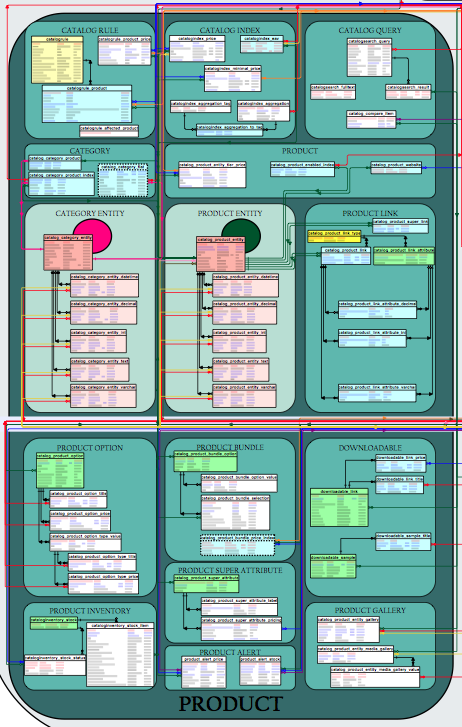
\includegraphics[width=0.3\textwidth]{figuras/cap2/magento_product_schema.png}
	\caption{\textit{Schemas}de un producto.}
	\label{cap:figure:catalog_magento}
\end{figure}

O realizar una sencilla búsqueda desde MongoDB JavaScript \textit{shell} para obtener un objecto \gloss{json} como este:

\medskip
\begin{lstlisting}[caption= Busqueda en MongoDB]

db.products.find({'_id': ObjectID("4bd87bd8277d094c458d2fa5")});

{_id: ObjectID("4bd87bd8277d094c458d2a43"),
 title: "A Love Supreme [Original Recording Reissued]"
 author: "John Coltrane",
 author_id: ObjectID("4bd87bd8277d094c458d2fa5"),

 details: {
   number_of_discs: 1,
   label: "Impulse Records",
   issue_date: "December 9, 1964",
   average_customer_review: 4.95,
   asin: "B0000A118M"
 },

 pricing: {
  list: 1198,
  retail: 1099,
  savings: 99,
  pct_savings: 8
 },

 categories: [
   ObjectID("4bd87bd8277d094c458d2a43"),
   ObjectID("4bd87bd8277d094c458d2b44"),
   ObjectID("4bd87bd8277d094c458d29a1")
 ]
}
\end{lstlisting}

Claramente no es una representación completa de un producto, pero esto demuestra cuantas de estas tablas triviales que existen en una \textit{relational representation} pueden prescindir en un \textit{document representation}.

Para \textit{object-oriented data}, los documentos tienen mayor sentido, tanto en concepto como rendimiento. Una representación \textit{document-oriented} de una \textit{data} de un producto se traduce a unas pocas entidades (un puñado de \textit{collections} vs. una docena de tablas), mejor \textit{performance} en consultas (sin \textit{sever-side joins}), y estructuras que corresponden precisamente al producto. Ya no existe la necesidad de diseñar un \textit{master schema} que pueda considerar a cada tipo de producto concebible.

\textit{Catalog management} es esencialmente \textit{content management}, un campo en donde MongoDB sobresale.

\subsection{Shopping Carts and Orders}

Permitir que un \textit{shopping cart} sea simplemente una orden en un estado del \textit{\"cart\"}, el modelo de \textit{shopping carts} y las ordenes en MongoDB se tornan muy sencillas:

\medskip
\begin{lstlisting}[caption= Estructura de una orden.]

{'_id': objectid('4b980a6dea2c3f4579da141e'),
 'user_id': objectid('4b980a6dea2c3f4579a4f54'),
 'state': 'cart',

 'line_items': [
    {'sku': 'jc-432',
     'name': 'John Coltrane: A Love Supreme',
     'retail_price': 1099
    },

    {'sku': 'ly-211',
     'name': 'Larry Young: Unity',
     'retail_price': 1199
    },
  ],

 'shipping_address': {
   'street': '3333 Greene Ave.',
   'city': 'Brooklyn',
   'state': 'NY',
   'zip': '11216'
  },

  'subtotal': 2199
}
\end{lstlisting}

Notar que es posible presentar los pedidos como un \textit{array} de productos. Como es usual con documentos, esto hace el despliegue del \textit{shopping cart} mas sencillo, dado que no hay \textit{joins} envueltos. Pero esto también resuelve el problema del versionamiento de productos. Usualmente es necesario tener el estado de un producto cuando este es comprado. Esto puede ser logrado en una \gloss{rdbms} estableciendo un vinculo a versiones particulares de un producto. Aquí, sin embargo, simplemente se almaceno el estado de un producto dentro de la misma orden.

\subsection{\textit{Querying Orders}}

Dado que MongoDB soporta consultas dinámicas y \textit{secondary indexes}, las consultas para las ordenes son automáticas. Es posible, por ejemplo, definir un \textit{index} en un \textit{product \gloss{sku}}, lo que permite consultas eficientes en todas las ordenes para un producto dado:

\medskip
\begin{lstlisting}[caption= Consulta eficiente con \textit{secondary indexes}.]
	db.orders.ensureIndex({'line_items.sku': 1});
	db.orders.find({'line_items.sku' => 'jc-431'});
\end{lstlisting}

Con MongoDB, es posible realizar consultas en atributos arbitrarios, de esa manera cualquier \textit{query}, en \textit{orders collection} es posible. Y para \textit{queries} comunes, es posible definir \textit{indexes} para una mejor eficiencia.

\subsection{\textit{Aggregation}}

Claramente, \textit{aggregation} también es necesario. Se desea reportar ordenes de diferentes maneras, y para ese propósito, \textit{map-reduce} esta disponible. Como ejemplo, el comando \textit{map-reduce} que \textit{aggregtes} el total de ordenes por \textit{zip code}:

\begin{lstlisting}[caption= Ejemplo de commando \textit{map-reduce}.]
map = "
  function() {
    emit(this['shipping_address']['zip'], {total: this.total})
  }"

reduce = "
  function(key, values) {
    var sum = 0;
    values.forEach(function(doc) {
      sum += doc.total;
    }

    return {total: sum};
  }"


db.orders.mapReduce(map, reduce, {out: 'order_totals_by_zip'});
\end{lstlisting}

\subsection{Updating Orders}

\subsubsection{Incrementing Quality}

Una manera de ajustar la cantidad es usando un \textit{position operator}, el cual permite aplicar \textit{atomic operations}, a un único objeto dentro de un \textit{array}. A continuación se muestra como cambiar el numero de álbumes que se están ordenando:

\begin{lstlisting}[caption= Ejemplo de \textit{atomic operation}.]
	db.orders.update({'_id': order_id, 'line_items.sku':'jc-431'},
		{'$set': {'line_items.$.quantity': 2}});
\end{lstlisting}

 
\subsubsection{Adding and Removing Items}

Igualmente, \textit{atomic operators} resuelven el problema de agregar y remover productos desde el carro. Por ejemplo, se puede utilizar \$push \textit{atomic operator} para agregar un item al \textit{cart};

\begin{lstlisting}[caption= Ejemplo de \textit{atomic operation}.]
	db.orders.update({'_id': order_id},
    {'$push': {'line_items':
      {'sku': 'md-12', 'price': 2500, 'title': 'Basketball'}}
     '$inc': {'subtotal': 2500}});
\end{lstlisting}

Al ajustar la cantidad y el cambio de los mismos \textit{items} en el \textit{cart}, es necesario actualizar el total de la orden. Notar el uso de \$inc \textit{operator} para manejar esto.

\subsection{Inventory}

No todos los sitios \textit{e-Commerce} necesitan manejar el inventario. Pero para aquellos que si lo hacen, MongoDB funciona a la altura de las circunstancias.

Una manera para manejar el inventario, es \textit{store} un documento separado por cada \textit{physical item} en la bodega. Así, por ejemplo, si la bodega tiene veinte copias del álbum Coltrane, se traduce en veinte documentos distintos en \textit{inventory collection}. Cada documento tiene una estructura como la siguiente:

\begin{lstlisting}[caption= Ejemplo de \textit{atomic operation}.]
	{'_id': objectid('4b980a6dea2c3f4579da432a'),
 'sku': 'jc-431',
 'state': 'available',
 'expires': null,
 'order_id': null
}
\end{lstlisting}


Cuando un usuario intenta agregar un \textit{item} al \textit{cart}, un \textit{findAndModify command} puede ser facilitado para \textit{atomically mark} el \textit{item} en \textit{in-cart}, asociando el \textit{item} con una orden dada, y estableciendo un tiempo de expiración:

\begin{lstlisting}[caption= Ejemplo de \textit{atomic operation}.]
	query = {'sku': 'jc-431', 'state': 'available'};

update = {'$set':
          {'state':    'cart',
           'order_id': order_id,
           'expires':  Date.now() + 15 * 60}};

item = db.inventory.findAndModify(query: query, update: update);
\end{lstlisting}

Si se obtiene un \textit{item back} desde el \textit{findAndModify operation}, se sabe que tenemos un único \textit{lock} en el \textit{item}, y es posible \textit{store it} en el \textit{cart}. Cuando el usuario desea \textit{check out}, el estado del \textit{item} puede cambiar a \textit{"purchased"}, o cualquiera sea el caso de la llamada.

Mientras, se pueda ejecutar un \textit{script in the background} que libere el inventario del \textit{cart} que no ha sido \textit{purchased} en la ventana de quince minutos. La actualización es trivial:

\begin{lstlisting}[caption= Ejemplo de \textit{atomic operation}.]
	db.inventory.update({'state': 'cart', 'expires': {'$lt': Date.now()}},
  {'$set' {'state': 'available', 'expires': null, 'order_id': null}},
  {multi: true});
\end{lstlisting} 

\subsection{\textit{Transactions}, \textit{Consistency} y \textit{Durability}}

Muchos argumentos impuestos contra NoSQL en \textit{e-Commerce} se centran en \textit{transactions}, \textit{consistency}, y \textit{durability}. En relación a esto se mencionan algunos puntos.

En relación a \textit{transactions}, ciertamente MongoDB no soporta el tipo \textit{multi-object}; sin embargo, soporta \textit{atomic operations} sobre documentos individuales. y esto combinado con \textit{documento-oriented modeling} recién descrito y creatividad, es suficiente para muchos problemas \textit{e-Commerce}. Ciertamente, si se necesita \textit{debit one account} y \textit{credit another} en la misma operación, o si se desea \textit{rollback}, sera necesario \textit{full-fledged transactions}. No obstante, \textit{transactionality} provista por MongodB debería ser suficiente en la mayoría de los casos, si no en todos, para \textit{e-Commerce operations}.

Si la preocupación esta sobre \textit{consistency} y \textit{durability}, operaciones escritas en MongoDB pueden ser realizadas \textit{consistency} sobre conexiones. Ademas, MongoDB 1.5 soporta \textit{near-real-time replications}, así que es posible asegurarse que una operación ha sido \textit{replicated} antes de retornar.

\subsection{\textit{Scalability}}
La manera mas sencilla para \textit{scale} la mayoría de las \textit{databases}, es \textit{upgrading} el \textit{hardware}. Si la aplicación esta corriendo en un único nodo, es usualmente posible agregar una combinación de \textit{disk} IOPS, \textit{memory}, y CPU para eliminar los cuello de botella de la \textit{database}.La técnica de mejorar el \textit{hardware} de un solo node para escalar se conoce como \textit{vertical scaling} o \textit{scaling up}. \textit{Vertical scaling} tiene la ventaja de ser simple, seguro, y \textit{cost-effective} hasta un cierto punto. Si se esta ejecutando sobre un \textit{virtualized hardware}( tal como \textit{Amazon's EC2}), entonces puedes encontrar que una instancia lo suficientemente larga no esta disponible. Si estas ejecutando sobre \textit{physical hardware}, habrá un punto donde el costo de un servidor mas poderoso se vuelve prohibitivo.

\begin{figure}[h!]
	\centering
	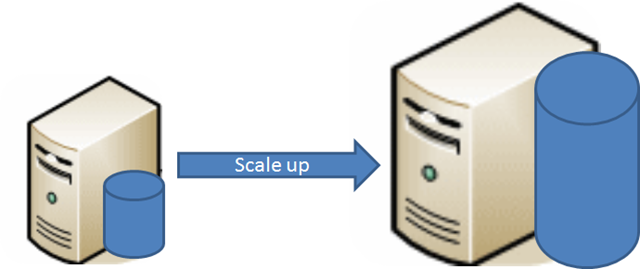
\includegraphics[width=0.5\textwidth]{figuras/cap2/scale_up.png}
	\caption{\textit{Vertical scaling} o \textit{Scaling up} }
\end{figure}

Entonces tiene sentido  considerar \textit{scaling horizontally} o \textit{scaling out}. En lugar de reforzar un único nodo, \textit{scalling horizontally} significa distribuir de \textit{database} sobre múltiples maquinas. Dado que \textit{horizontally scaled architecture} puede utilizar \textit{comodity hardware}, el costo de \textit{hosting} el total de la \textit{data} puede ser reducido significativamente. Incluso, la distribución  de \textit{data} sobre maquinas mitiga las consecuencias de fallo. Las maquinas inevitablemente fallaran de algún momento a otro. Si se \textit{scaled vertically} , y la maquina falla, entonces es necesario tratar con una falla en un maquina de la cual la mayoría del sistema depende. Podría no considerarse un tema si una copia de la \textit{data} existe en un \textit{replicated slave}, pero aun esta el caso e que solo un único \textit{sever} es necesario para bajar el sistema completo. En contraste con el fallo dentro de un \textit{horizontally scaled architecture}. Esto podría ser menos catastrófico dado que una sola máquina representa un porcentaje menor del sistema completo.

\begin{figure}[h!]
	\centering
	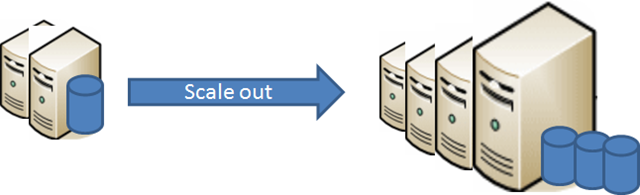
\includegraphics[width=0.5\textwidth]{figuras/cap2/scale_out.png}
	\caption{\textit{Horizontally scaling} o \textit{Scaling out} }
\end{figure}

MongoDB es un \textit{database management system} diseñado para hacer \textit{horizontal scaling} manejable, dado que fue construido para aplicaciones \textit{web} e infraestructuras de Internet.

\subsection{Conclusion}

Es cierto que la mayoría de \textit{NoSQL databases} no fueron construidas considerando \textit{e-Commmerce}. \textit{Databases} que carecen \textit{data models} enriquecidos, \textit{dynamic queries}, y la noción de \textit{transactionality} no puede esperarse que compitan en el espacio de \textit{e-Commerce}, entonces no es comprensible que no se considere MongoDB tampoco.

Pero para las partes en donde el sitio \textit{\gloss{ecommerce}} comprende el manejo de contenido, MongoDB es claro vencedor. E incluso para mas \textit{transactional components} del sistema, MongoDB tiene características que hacen de la posibilidad de correr un sistema completo de \textit{e-Commerce} una realidad.

\section{Resumen}

Recapitulando, he demostrado que las soluciónes actuales de ecommerce pueden ser considerablemente mejoradas utilizando la tecnología actualmente presente. 
Importante notar que solo estoy ofreciendo una mejor solucuón a lo que ya existe, en ningun caso indico la solución que presento es la mejor posible. No se ha realizado un estudio sobre todas las opciones disponibles del mercado. Sin embargo esta solución ofrece

speed
scalability
flexibility
performance

%
\chapter{Justificación del proyecto}\label{cap:justificacion_proyecto}

%\subsection{Nueva tecnología no es sinónimo de mejores soluciones}
%TODO

A continuación se discutirán las razones para considerar el desarrollo de una plataforma \ecommerce un aporte en relación a las opciones \opensource actualmente vigentes. Para esto se explicara por que los cambios de tecnología propuestos son un beneficio para el actual estado del arte del tema, así como un aporte para potenciales funcionalidades que serán agregadas en el futuro.

%TODO Hablar de arquitectura de proyecto para luego diferenciar las diferentes tecnologias y explicar cual es la mas adecuada en cada caso.

\section{Base de datos}

Bases de datos relacionales se encuentran en la mayoría de las organización desde hace muchísimo tiempo, y por buenas razones. Las bases de datos relacionales soportan las aplicaciones del pasado que cumplen con las necesidades de negocio actuales; Estas son apoyadas por un extenso ecosistema de herramientas; y hay una gran cantidad de mano de obra calificada para implementar y mantener estos sistemas.
%Relational databases have a long-standing position in most
%organizations, and for good reason. Relational databases
%underpin legacy applications that meet current business
%needs; they are supported by an extensive ecosystem of
%tools; and there is a large pool of labor qualified to
%implement and maintain these systems.

Pero las compañías están cada vez mas considerando la opción de alternativas para la infraestructura relacional heredada. En algunos casos la motivación es técnica, tal como la necesidad de escalar o actuar mas allá de las capacidades de sus sistemas actuales. Mientras que en otros casos, las compañías están motivadas por el deseo de identificar alternativas viables a \textit{softwares} propietario de alto costo. Una tercera motivación es la agilidad y velocidad del desarrollo, dado que las compañías ansían adaptarse al mercado mas rápido y adoptar metodologías de desarrollo ágil.
%But companies are increasingly considering alternatives to
%legacy relational infrastructure. In some cases the
%motivation is technical — such as a need to scale or
%perform beyond the capabilities of their existing systems —
%while in other cases companies are driven by the desire to
%identify viable alternatives to expensive proprietary
%software. A third motivation is agility or speed of
%development, as companies look to adapt to the market
%more quickly and embrace agile development
%methodologies.


%TODO revizar este parrafo
Estas opciones se aplican tanto para aplicaciones \gloss{analytic_processing} como \gloss{tarnsactional_processing}. Las compañías están cambiando \textit{workloads} a \textit{Hadoop} \ref{ap:apendice_hadoop_description} para sus \textit{offline}, \textit{analytical workloads}, y están construyendo \textit{online}, aplicaciones operacionales con una nueva clase de tecnología de manejo de datos llamada "\gloss{nosql}", como por ejemplo \gloss{mongodb}.
%These drivers apply both to analytical and transactional applications. Companies are shifting workloads to Hadoop for their offline, analytical workloads, and they are building online, operational applications with a new class of data management technologies called "NoSQL", or "Not Only SQL", such as MongoDB

\subsection{\gloss{sql} and the Relational Model}

\gloss{sql} es un lenguaje declarativo de consulta de datos. Un lenguaje declarativo es uno en el cual un programador especifica lo que desea y el sistema lo ejecuta, en lugar de definir proceduralmente como el sistema debería hacerlo. Unos pocos ejemplos incluyen: encontrar el registro del \textit{estudiante} 39, mostrar solo el \textit{nombre} y el \textit{número de teléfono} del estudiante de la totalidad de su registro, filtrar los registros de los \textit{estudiantes} a aquellos que cursan contabilidad, contar la cantidad de \textit{estudiantes} en cada curso, unir la información de la tabla de los \textit{estudiantes} con la tabla de \textit{profesores}.
%SQL is a declarative language for querying data. A declarative language is one in which a programmer specifies what they want the system to do, rather than procedurally defining how the system should do it. A few examples include: find the record for employee 39, project out only the employee name and phone number from their entire record, filter employee records to those that work in accounting, count the employees in each department, or join the data from the employees table with the managers table.


En una primera aproximación, \gloss{sql} permite consultar sobre aquellas preguntas sin pensar sobre como la información es expuesta en el disco, cuales indices utilizar para acceder a la información o que algoritmo utilizar para procesar la información. Un componente arquitectural significativo para la mayoría de las bases de datos relacionales es un optimizador de consultas, el cual decide cual de las muchos equivalentes lógicos planea ejecutar para obtener la respuesta mas rápida a una consulta. Estos optimizadores son usualmente mejores que los promedios de los usuarios de la base de datos, pero en algunas ocasiones estos no tienen la suficiente información o tienen un modelo muy simple del sistema con el fin de generar la ejecución mas eficiente.
%To a first approximation, SQL allows you to ask these questions without thinking about how the data is laid out on disk, which indices to use to access the data, or what algorithms to use to process the data. A significant architectural component of most relational databases is a query optimizer, which decides which of the many logically equivalent query plans to execute to most quickly answer a query. These optimizers are often better than the average database user, but sometimes they do not have enough information or have too simple a model of the system in order to generate the most efficient execution.

Bases de datos relacionales, las bases de datos mas utilizadas en la practica, siguen el modelo de datos relacional. En este modelo, diferentes entidades del \textit{real-world} son guardadas en diferentes tablas. Por ejemplo, todos los \textit{estudiantes} podrían ser guardados en una tabla \textit{Estudiantes}, y todos los \textit{cursos} podrían ser almacenados en la tabla \textit{Cursos}. Cada fila de una tabla tiene varias propiedades guardadas en columnas. Por ejemplo, \textit{estudiantes} podrían tener un \textit{estudiantes id}, \textit{dirección}, \textit{edad},  \textit{fecha nacimiento}, y \textit{nombres/apellidos}. Cada una de estas propiedades sera guardada en una columna de la tabla \textit{Estudiantes}
%Relational databases, which are the most common databases used in practice, follow the relational data model. In this model, different real-world entities are stored in different tables. For example, all employees might be stored in an Employees table, and all departments might be stored in a Departments table. Each row of a table has various properties stored in columns. For example, employees might have an employee id, salary, birth date, and first/last names. Each of these properties will be stored in a column of the Employees table.


El modelo relacional, va mano a mano con \gloss{sql}. Consultas simples de \gloss{sql}, tales como filtrar, recuperar todos los registros el cual sus campos hagan \textit{match} en algunos test (ejemplo, \textit{estudiante id} = 3, o edad > 20 años). Construcciones mas complejos causan que la base de datos haga trabajo extra, tal como \textit{joining} información sobre múltiples tablas (ejemplo., ¿ Cuales son los nombres de los cursos que actualmente tiene inscritos el \textit{estudiante id} 3 ?). Otras estructuras complejas tal como \textit{aggregates} (ejemplo, ¿ cuál es la cantidad promedio de ramos que tiene inscrito los estudiantes
?) pueden conducir a realizar un \textit{scan} completo de la tabla.
%The relational model goes hand-in-hand with SQL. Simple SQL queries, such as filters, retrieve all records whose field matches some test (e.g., employeeid
% = 3, or salary \> \$ 20000). More complex constructs cause the database to do some extra work, such as joining data from multiple tables (e.g., what is the name of the department in which employee 3 works?). Other complex constructs such as aggregates (e.g., what is the average salary of my employees?) can lead to full-table scans.


Un modelo de datos relacional define entidades altamente estructuradas con relaciones estrictas entre ellos. Consultar este modelo con \gloss{sql} permite recorridos de datos complejos sin demasiado desarrollo personalizado. La complejidad del modelo y las consultas, tienen sus limites, aunque:
%The relational data model defines highly structured entities with strict relationships between them. Querying this model with SQL allows complex data traversals without too much custom development. The complexity of such modeling and querying has its limits, though:


\textit{Complexity} guía a \textit{unpredictability}. La expresividad en \gloss{sql} implica un desafío en relación al costo de cada consulta, y así el costo de \textit{\glos{workload}}. Mientras lenguajes de consultas simples pueden complicar la lógica, al mismo tiempo hacen que sea sencillo proveer de almacenamiento de datos, cuando solo responde a consultas simples.
%Complexity leads to unpredictability. SQL's expressiveness makes it challenging to reason about the cost of each query, and thus the cost of a workload. While simpler query languages might complicate application logic, they make it easier to provision data storage systems, which only respond to simple requests.

Hay muchas maneras de modelar un problema. El modelo de datos relacional es estricto: El esquema asignado para cada tabla especifica los datos en cada fila. Si se están almacenando menos datos estructurados, o filas con mas diferencia en las columnas que se guardan,el modelo relacional puede ser innecesariamente restrictivo. Similarmente, aplicaciones desarrolladas podrían no encontrar el modelo relacional idóneo para modelar cada tipo de dato. Por ejemplo, una gran cantidad den aplicaciones lógicas son escritas en lenguaje \textit{object-oriented} e incluye conceptos \textit{high-level} tales como \textit{lists}, \textit{queues}, y \textit{sets}, y algunos programadores desearan \textit{persistence layer} para modelar esto.
%There are many ways to model a problem. The relational data model is strict: the schema assigned to each table specifies the data in each row. If we are storing less structured data, or rows with more variance in the columns they store, the relational model may be needlessly restrictive. Similarly, application developers might not find the relational model perfect for modeling every kind of data. For example, a lot of application logic is written in object-oriented languages and includ-es high-level concepts such as lists, queues, and sets, and some programmers would like their persistence layer to model this.

Si los datos crecen mas allá de la capacidad de un servidor, entonces las tablas en la base de datos tendrán que ser particionadas a través de varios computadores. Para evitar \textit{JOINs} a través de la red para obtener todas las tablas requeridas, será necesario desnormalizarla. Desnormalizar consiste en guardar todos los datos de diferentes tablas que se desean consultar en el mismo lugar. Esto hace que la base de datos simule una \textit{key-lookup store system}, dejando preguntas sobre la posibilidad de adaptarse mejor a los datos.
%If the data grows past the capacity of one server, then the tables in the database will have to be partitioned across computers. To avoid JOINs having to cross the network in order to get data in different tables, we will have to denormalize it. Denormalization stores all of the data from different tables that one might want to look up at once in a single place. This makes our database look like a key-lookup storage system, leaving us wondering what other data models might better suit the data.

Generalmente no es inteligente descartar años de consideraciones de diseño arbitrariamente. Cuando se considera el almacenamiento de los datos en una base de datos, considera \gloss{sql} y el modelo relacional, los cuales son respaldados por décadas  de investigación y desarrollo, ofreciendo enriquecidas capacidades de modelamiento, y proporcionan garantías \textit{fácil-de-entender} sobre operaciones complejas. \gloss{nosql} es una buena opción cuando se tiene un problema específico, tal como gran cantidad de datos, un masivo \textit{workload}, o una difícil decisión de modelamiento para la cual \gloss{sql} y bases de datos relacionales podrían no haber sido optimizadas.
%It's generally not wise to discard many years of design considerations arbitrarily. When you consider storing your data in a database, consider SQL and the relational model, which are backed by decades of research and development, offer rich modeling capabilities, and provide easy-to-understand guarantees about complex operations. NoSQL is a good option when you have a specific problem, such as large amounts of data, a massive workload, or a difficult data modeling decision for which SQL and relational databases might not have been optimized.

\subsection{NoSQL}

\gloss{nosql} engloba una gran variedad de diferentes tecnologías de bases de datos y fueron desarrolladas en respuesta al creciente volumen de datos guardados de los usuarios, objetos y productos, la frecuencia en que los datos son accesados, y la \textit{performance} en las necesidades de los procesos. Bases de datos relacionales, por otra parte, no fueron diseñadas para hacer frente a los desafíos de \textit{escalabilidad} y \textit{agilidad} que enfrentan las aplicaciones modernas, no fueron construidas para tomar ventaja del almacenamiento barato y el poder de procesamiento disponible en la actualidad.
%NoSQL encompasses a wide variety of different database technologies and were developed in response to a rise in the volume of data stored about users, objects and products, the frequency in which this data is accessed, and performance and processing needs. Relational databases, on the other hand, were not designed to cope with the scale and agility challenges that face modern applications, nor were they built to take advantage of the cheap storage and processing power available today.

\subsubsection{Document Model}\label{cap:justificacion_proyecto:base_datos:nosql:document_model}

 Mientras las bases de datos relacionales guardan la información en filas y columnas, \textit{document databases} guardan los datos en documentos.  

Estos documentos tipicamente usan una estructura equivalente a \json, un formato muy popular entre desarrolladores. Los documentos proveen una manera intuitiva y natural para modelar datos que esta cercanamente alineada con la programación \textit{object-oriented}, en el cual cada documento es efectivamente un objeto. Los documentos contienen uno o mas campos, donde cada campo contiene un tipo de valor, tales como \textit{string}, \textit{date}, \textit{binary}, o \textit{array}. En lugar de extenderse un registro entre múltiples tablas y columnas, cada registro y su dato asociado son tipicamente almacenados juntos en un solo documento. Esto simplifica el acceso a la información y reduce e incluso elimina la necesidad de \joins y\textit{complex transactions}.

En un \textit{document database}, la noción de esquema es dinámica: cada documento puede contener diferentes campos. Esta flexibilidad puede ser particularmente útil para modelar datos sin estructura y \textit{polymorphic}. Esto también hace posible la evolución de una aplicación durante su desarrollo, simplemente agregando nuevos campos. Adicionalmente, \textit{document databases} generalmente proveen consultas robustas que los desarrolladores esperan en las bases de datos relacionales.

Aplicaciones:\textit{Document databases} son de propósito general y útiles para una amplia variedad de aplicaciones, debido a su flexibilidad del modelo de datos, la habilidad para consultar sobre cualquier campo y el \textit{natural mapping} del \textit{document data model} a objetos en programación de lenguajes modernos.

Ejemplos: MongoDB y CouchDB.

\subsubsection{Graph Model}
\label{cap:justificacion_proyecto:base_datos:nosql:graph_model}

Basado en \nameref{ap:apendice_graph_theory}, usa estructuras de grafos con nodos, bordes y propiedades para representar los datos. En esencia, los datos son modelados como una red de relaciones entre elementos específicos. Si bien es cierto, \textit{Model Graph}, puede ser contra intuitivo y tomar tiempo para entenderlo, puede ser utilizado extensamente para numerosas aplicaciones. Su principal característica es que modela fácilmente las relaciones entre entidades en una aplicación.

Aplicaciones:\textit{Graph databases} son útiles en escenarios donde las relaciones son el \textit{core} de la aplicación, como redes sociales.

Ejemplos: Neo4j y HyperGraphDB.

\subsubsection{Key-Value}
\label{cap:justificacion_proyecto:base_datos:nosql:key_value}

Desde una perspectiva de modelo de datos, \textit{key-value stores} son el tipo mas básico de las \textit{\gloss{nosql} databases}. Cada \textit{item} en la base de datos es guardado como un atributo \textit{name}, ó \textit{key}, junto con su \textit{value}. El \textit{value}, sin embargo, es totalmente \textit{opaque} al sistema; los datos solo pueden ser requeridos desde la \textit{key}. Este modelo puede ser útil para representar \textit{polymorphic} y datos \textit{unstructured}, dado que la base de datos  no define un esquema al conjunto \textit{key-value}.
%From a data model perspective, key-value stores are the most basic type of NoSQL database. Every item in the database is stored as an attribute name, or key, together with its value. The value, however, is entirely opaque to the system; data can only be queried by the key. This model can be useful for representing polymorphic and unstructured data, as the database does not enforce a set schema across key-value pairs.

\subsubsection{Wide Column Models}
\label{cap:justificacion_proyecto:base_datos:nosql:wide_column_model}

%TODO falta mejorar esta definición
\textit{Wide Column stores}, ó \textit{colum family stores}, \textit{use a sparse}, mapa ordenado \textit{multi-dimensional} distribuido para guardar datos. Cada registro puede variar en el numero de \textit{columns} que son guardadas, y las \textit{columns} pueden ser anidadas dentro de otras \textit{columns} llamadas \textit{super columns}. \textit{Columns} pueden ser agrupadas juntas por acceso en \textit{column families}, o \textit{columns} pueden ser propagadas a través de múltiples \textit{column families}. Los datos son recuperados por \textit{primary key} por \textit{column family}.
%Wide column stores, or column family stores, use a sparse, distributed multi-dimensional sorted map to store data. Each record can vary in the number of columns that are stored, and columns can be nested inside other columns called super columns. Columns can be grouped together for access in column families, or columns can be spread across multiple column families. Data is retrieved by primary key per column family.

Aplicación: \textit{Key value stores} y \textit{wide column stores} son útiles para un reducido conjunto de aplicaciones que solo consultan datos para un único \textit{key value}. Lo llamativo de estos sistemas es su \textit{performance} y \textit{scalability}, los cuales pueden ser \textit{highly optimized} debido a su simplicidad de los patrones de acceso de datos.
%Applications: Key value stores and wide column stores are useful for a narrow set of applications that only query data by a single key value. The appeal of these systems is their performance and scalability, which can be highly optimized due to the simplicity of the data access patterns.

%Examples: Riak and Redis (Key-Value); HBase and Cassandra (Wide Column).


\begin{table}[h!]
    \tiny
   
%\begin{tabular}{ |C{0.3\paperwidth}|C{0.3\paperwidth}| }
\begin{tabular}{ |L{0.1\paperwidth}|L{0.3\paperwidth}|L{0.3\paperwidth}|}
\hline
	&
	\gloss{sql} Databases &
	\gloss{nosql} Databases
 
\\ \hline
	Tipos&%Types
	Un tipo (\gloss{sql} Database) con variacions menores.& %One type (SQL database) with minor variations&
	Muchos tipos distintos incluyendo \nameref{cap:justificacion_proyecto:base_datos:nosql:key_value}, \nameref{cap:justificacion_proyecto:base_datos:nosql:document_model}, \nameref{cap:justificacion_proyecto:base_datos:nosql:wide_column_model}, y \nameref{cap:justificacion_proyecto:base_datos:nosql:graph_model}. %Many different types including key-value stores, document databases, wide-column stores, and graph databases
	
\\ \hline
	Historia de desarrollo&%Development History&
	Desarrollado en 1970s para tratar con la primera ola de aplicaciones de almacenamiento de \textit{data}.&%Developed in 1970s to deal with first wave of data storage applications&
	Desarrollado en 2000s para tratar con las limitaciones de las bases de datos \gloss{sql}, en particular en relación a \textit{scale}, \textit{replication} y guardar datos sin estructura.%Developed in 2000s to deal with limitations of SQL databases, particularly concerning scale, replication and unstructured data storage
	
\\ \hline
	Ejemplos&%Examples&
	MySQL, Postgres, Oracle \textit{Database}&
	MongoDB, Cassandra, HBase, Neo4j
\\ \hline
	\textit{Data Storage Model}&
	Registros individuales ( ej., \"employees\") son guardados como filas en la tabla, con cada columna guardando un dato específico sobre el registro (ej., \"manager\", \"data hired\", etc), similar a un \textit{spreedsheet}. Tipos de datos separados son guardados en tablas separadas, y entonces uniéndose cuando consultas mas complejas son ejecutadas. Por ejemplo, "offices" podrían estar guardadas en una tabla, y \"employees\" en otra. Cuando un usuario quiere buscar la dirección de trabajo de un \textit{employee}, el \textit{database engine} \joins las tablas \"employee\" y \"office\" juntas para obtener toda la información necesaria.&
	%Individual records (e.g., "employees") are stored as rows in tables, with each column storing a specific piece of data about that record (e.g., "manager," "date hired," etc.), much like a spreadsheet. Separate data types are stored in separate tables, and then joined together when more complex queries are executed. For example, "offices" might be stored in one table, and "employees" in another. When a user wants to find the work address of an employee, the database engine joins the "employee" and "office" tables together to get all the information necessary.&
	
	Varia de acuerdo al tipo de base de datos. Por ejemplo, \textit{key-value store} funciona de manera similar a la base de datos \sql, pero tiene solo dos \columns (\"key\" y \"value\"), con información mas compleja en algunas ocasiones guardada dentro de \columns \"value\". \textit{Document databases} acabó con el \textit{table-and-row model} completamente, guardando todos los datos relevantes junto en un solo \textit{\"document\"} en \json, \xml, u otro formato, el cual puede anidar valores jerárquicamente.
	%Varies based on database type. For example, key-value stores function similarly to SQL databases, but have only two columns ("key" and "value"), with more complex information sometimes stored within the "value" columns. Document databases do away with the table-and-row model altogether, storing all relevant data together in single "document" in JSON, XML, or another format, which can nest values hierarchically.
	

\\ \hline
	\textit{Schemas}&
	%Schemas&
	
	Estructura y tipo de datos son fijos por adelantado. Para guardar información sobre un nuevo \textit{data item}, la base de datos entera debe ser alterada, tiempo durante el cual la base de datos debe ser tomada \textit{offline}.&
%	Structure and data types are fixed in advance. To store information about a new data item, the entire database must be altered, during which time the database must be taken offline.&

	Tipicamente dinámica. Registros pueden agregar nueva información \textit{on the fly}, y diferente a \textit{\gloss{sql} table rows}, datos distintos pueden estar guardados juntos como sea necesario. Para algunas \textit{databases} (ej., \textit{wide-column stores}), es algo mas desafiante para agregar nuevos \textit{fields dinamically}.
	%Typically dynamic. Records can add new information on the fly, and unlike SQL table rows, dissimilar data can be stored together as necessary. For some databases (e.g., wide-column stores), it is somewhat more challenging to add new fields dynamically.

\\ \hline
	\textit{Scaling}&%Scaling&
	
	\textit{Vertivally}, significa que un solo servidor debe incrementar \textit{powerful} con el fin de hacer frente al incremento de demanda. Es posible propagar la base de datos \gloss{sql} sobre muchos servidores, pero ingeniería significativa adicional será generalmente requerida.&
	%Vertically, meaning a single server must be made increasingly powerful in order to deal with increased demand. It is possible to spread SQL databases over many servers, but significant additional engineering is generally required.&
	
	\textit{Horizontally}, significa que para agregar capacidad, un administrador de base de datos puede simplemente agregar mas servidores o \textit{cloud instances}.
	%Horizontally, meaning that to add capacity, a database administrator can simply add more commodity servers or cloud instances. The database automatically spreads data across servers as necessary.
	
\\ \hline
	\textit{Development Model}&
	%Development Model&
	
	\textit{Mix} de \opensource (ej., Postgres, MySQL) y \textit{closed source} (ej., Oracle \textit{Database})&
	%Mix of open-source (e.g., Postgres, MySQL) and closed source (e.g., Oracle Database)&
	\opensource
	%Open-source
	
\\ \hline
	\textit{Supports Transactions}&
	%Supports Transactions&
	
	Si, actualizaciones pueden ser configuradas para completar enteramente o no del todo&	
	%Yes, updates can be configured to complete entirely or not at all&
	
	En ciertas circunstancias y en ciertos niveles (ej., \textit{document level} vs. \textit{database level})
	%In certain circumstances and at certain levels (e.g., document level vs. database level)
	
\\ \hline
	\textit{Data Manipulation}&
	%Data Manipulation&
	
	Lenguaje especial usando \textit{Select}, \textit{Insert}, y \textit{Update statements}, ej., SELECT fields FROM table WHERE...&	
	%Specific language using Select, Insert, and Update statements, e.g. SELECT fields FROM table WHERE…&
	
	A través de APIs \textit{object-oriented}
	%Through object-oriented APIs

\\ \hline

	\textit{Consistency}&
	%Consistency&
	
	Puede ser configurada para \textit{strong consistency}&
	%Can be configured for strong consistency&
	
	Depende del producto. Algunos proveen \textit{strong consistency} (ej., \mongodb) mientras otros ofrecen \textit{eventual consistency} (ej., Cassandra)
	%Depends on product. Some provide strong consistency (e.g., MongoDB) whereas others offer eventual consistency (e.g., Cassandra)

\\ \hline
\end{tabular}
    \caption{ Resumen \nosql vs. \sql}
    \label{tab:SQL_vs_noSQL_summary}
\end{table}

\subsection{\mongodb y \ecommerce \cite{online_mongodb_ecommerce}}
\label{cap:justificacion_proyecto:MongoDB_ECommerce}

Demostraciones de almacenamientos de datos de la siguiente generación giran típicamente en torno a las redes sociales: \twitter, \facebook, \foursquare, etc. Desafortunadamente, tales aplicaciones generalmente tienen modelos de datos complejos. \ecommerce por ejemplo, tiene la ventaja de incluir un largo número de patrones familiares para modelar datos. Ademas no es complicado imaginar como \textit{products}, \textit{categories}, \textit{product reviews} y \textit{orders} son típicamente modeladas en \rdbms.

\ecommerce ha sido usualmente un dominio exclusivo de \rdbms, y esto es así por un par de razones. La primera, es que los sitios \ecommerce generalmente requieren \textit{transactions}, y \textit{transactions} son una operación básica en \rdbms. Lo segundo es que, hasta hace poco, dominios que requieren de un modelo de dato enriquecido y consultas sofisticadas han sido presupuestos que se ajustan mejor en \rdbms. En las siguientes secciones se cuestionara la segunda afirmación. 

\subsubsection{\textit{Catalog Management}}

Si es necesaria información sobre como el \textit{catalog management} se maneja con bases de datos relacionales, es necesario dar una mirada rápida a los esquemas del popular Magento \ecommerce \framework \ref{ap:figure:catalog_magento} ó OfBiz de Apache \ref{ap:figure:catalog_ofbiz}. En la \refFigura{cap:figure:catalog_magento}  se observa es un conjunto de tablas trabajando a la par para proveer un esquema flexible sobre un fundamentalmente inflexible estilo de sistema de base de datos.

Esto significa que los datos de cualquier producto se extienden a través de una docena de tablas. Esto incremente la complejidad del código requerido para la persistencia de consultas de productos individuales y hacer una consulta \textit{shell-based} es casi imposible. Simplemente considere escribir un \sql \join para para reunir el modelo de un producto como el de la \refFigura{cap:figure:catalog_magento}.

\begin{figure}[h!]
	\centering
	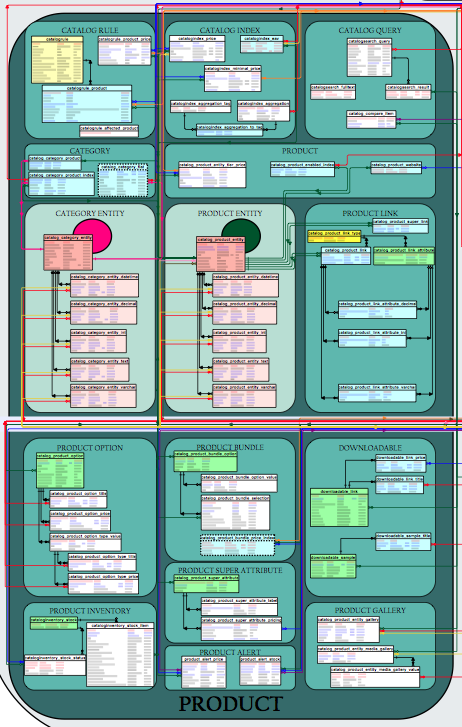
\includegraphics[width=0.3\textwidth]{figuras/cap2/magento_product_schema.png}
	\caption{Esquemas de un producto.}
	\label{cap:figure:catalog_magento}
\end{figure}

O realizar una sencilla búsqueda desde la \textit{shell} \mongodb \javascript  para obtener un objecto \json como el \refsource{source:javascript:example_search_mongodb}.

\medskip
\begin{lstlisting}[caption= Busqueda en MongoDB, label=source:javascript:example_search_mongodb]

db.products.find({'_id': ObjectID("4bd87bd8277d094c458d2fa5")});

{
	_id			: ObjectID("4bd87bd8277d094c458d2a43"),
	title		: "A Love Supreme [Original Recording Reissued]"
	author		: "John Coltrane",
	author_id	: ObjectID("4bd87bd8277d094c458d2fa5"),
	details		: {
					number_of_discs: 1,
					label: "Impulse Records",
   					issue_date: "December 9, 1964",
   					average_customer_review: 4.95,
   					asin: "B0000A118M"
   				},
   	pricing		: {
   					list: 1198,
   					retail: 1099,
   					savings: 99,
   					pct_savings: 8
   				},
   categories	: [
   					ObjectID("4bd87bd8277d094c458d2a43"),
   					ObjectID("4bd87bd8277d094c458d2b44"), 
   					ObjectID("4bd87bd8277d094c458d29a1")
   				]
}
\end{lstlisting}

Claramente en \refsource{source:javascript:example_search_mongodb} no hay  representación completa de un producto, pero esto demuestra cuantas de estas tablas triviales que existen en una representación relacional pueden prescindir en un \textit{document representation}.

Para datos \textit{object-oriented}, los documentos tienen mayor sentido, tanto en concepto como rendimiento. Una representación \textit{document-oriented} de un dato de un producto se traduce a unas pocas entidades (un puñado de \textit{collections} vs. una docena de tablas), mejor \textit{performance} en consultas (sin \textit{sever-side} \joins), y estructuras que corresponden precisamente al producto. Ya no existe la necesidad de diseñar un \textit{master schema} que pueda considerar a cada tipo de producto concebible.

\textit{Catalog management} es esencialmente \textit{content management}, un campo en donde MongoDB sobresale.

\subsubsection{Shopping Carts and Orders}

Permitir que un \textit{shopping cart} sea simplemente una orden en un estado  \textit{"cart"}, el modelo de \textit{shopping carts} y las ordenes en MongoDB se tornan muy sencillas. Un ejemplo de esto se puede observar en  \refsource{source:javascript:example_schema_order}.

\medskip
\begin{lstlisting}[caption= Estructura de una orden., label=source:javascript:example_schema_order]

{
	'_id': objectid('4b980a6dea2c3f4579da141e'),
	'user_id': objectid('4b980a6dea2c3f4579a4f54'),
	'state': 'cart',
	'line_items': [
		{
			'sku': 'jc-432',
			'name': 'John Coltrane: A Love Supreme',
			'retail_price': 1099
		},
		{
			'sku': 'ly-211',
			'name': 'Larry Young: Unity',
			'retail_price': 1199
		}
	],
	'shipping_address': {
		'street': '3333 Greene Ave.',
		'city': 'Brooklyn',
		'state': 'NY',
		'zip': '11216'
	},
	'subtotal': 2199
}
\end{lstlisting}

Notar que es posible presentar los pedidos como un \textit{array} de productos. Como es usual con documentos, esto hace el despliegue del \textit{shopping cart} mas sencillo, dado que no hay \joins envueltos. Pero esto también resuelve el problema del versionamiento de productos. Usualmente es necesario tener el estado de un producto cuando este es comprado. Esto puede ser logrado en una \rdbms estableciendo un vinculo a versiones particulares de un producto. Aquí, sin embargo, simplemente se almaceno el estado de un producto dentro de la misma orden.

\subsubsection{\textit{Querying Orders}}

Dado que MongoDB soporta consultas dinámicas y \textit{secondary indexes}, las consultas para las ordenes son automáticas. Es posible, por ejemplo, definir un \textit{index} en un \textit{product \gloss{sku}}, lo que permite consultas eficientes en todas las ordenes para un producto dado. En  \refsource{source:javascript:example_querying_orders_mongodb} se observa un ejemplo.

\medskip
\begin{lstlisting}[caption= Consulta eficiente con \textit{secondary indexes}., label=source:javascript:example_querying_orders_mongodb]

	db.orders.ensureIndex({'line_items.sku': 1});
	db.orders.find({'line_items.sku' => 'jc-431'});
	
\end{lstlisting}

Con MongoDB, es posible realizar consultas en atributos arbitrarios, de esa manera, cualquier consulta en \textit{orders collection} es posible. Y para consultas comunes, es posible definir \textit{indexes} para una mejor eficiencia.

\subsubsection{\textit{Aggregation}}

Claramente, \textit{aggregation} también es necesario. Se desea reportar ordenes de diferentes maneras, y para ese propósito, \textit{map-reduce} esta disponible. A modo de ejemplo,  \refsource{source:javascript:example_aggregation_mongodb} tiene comando \textit{map-reduce} que \textit{aggregtes} el total de ordenes por \textit{zip code}.

\begin{lstlisting}[caption= Ejemplo de commando \textit{map-reduce}., label=source:javascript:example_aggregation_mongodb]

map = "
	function(){
		emit(this['shipping_address']['zip'], {total: this.total})
	}
"

reduce = "
	function(key, values) {
		var sum = 0;
		values.forEach(function(doc) {
      sum += doc.total;
    }

    return {total: sum};
  }"


db.orders.mapReduce(map, reduce, {out: 'order_totals_by_zip'});

\end{lstlisting}

\subsubsection{Updating Orders}

\subsubsection*{Incrementing Quality}

Una manera de ajustar la cantidad es usando un \textit{position operator}, el cual permite aplicar \textit{atomic operations}, a un único objeto dentro de un \textit{array}. \refsource{source:javascript:example_incrementing_quality_mongodb} muestra como cambiar el número de álbumes que se están ordenando.

\begin{lstlisting}[caption= Ejemplo de uso de \textit{position operator}., label=source:javascript:example_incrementing_quality_mongodb]

	db.orders.update(
		{
			'_id': order_id,
			'line_items.sku':'jc-431'
		},
		{
			'$set': {'line_items.$.quantity': 2}
		}
	);
		
\end{lstlisting}

 
\subsubsection*{Adding and Removing Items}

Igualmente, \textit{atomic operators} resuelven el problema de agregar y remover productos desde el carro. \refsource{source:javascript:example_push_operator_mongodb} ejemplifica el uso de \$push \textit{atomic operator} para agregar un item al \textit{cart}.

\begin{lstlisting}[caption= Ejemplo del operador \$push., label=source:javascript:example_push_operator_mongodb]
db.orders.update(
	{'_id': order_id},
    {
    	'$push': {
    		'line_items':{
    			'sku': 'md-12',
    			'price': 2500,
    			'title': 'Basketball'
    		}
    	},
    	'$inc': {'subtotal': 2500}
    }
);
\end{lstlisting}

Al ajustar la cantidad y el cambio de los mismos \textit{items} en el \textit{cart}, es necesario actualizar el total de la orden. Notar el uso de \$inc \textit{operator} para manejar esto.

\subsubsection{Inventory}

No todos los sitios \ecommerce necesitan manejar el inventario. Pero para aquellos que si lo hacen, \gloss{mongodb} funciona a la altura de las circunstancias.

Una manera para manejar el inventario, es guardar un documento separado por cada \textit{physical item} en la bodega. Así, por ejemplo, si la bodega tiene veinte copias del álbum Coltrane, se traduce en veinte documentos distintos en \textit{inventory collection}. Cada documento tiene una estructura como lo muestra \refsource{source:javascript:example_document_inventory_mongodb}.

\begin{lstlisting}[caption= Ejemplo de documento para un \textit{item}., label=source:javascript:example_document_inventory_mongodb]
{
	'_id': objectid('4b980a6dea2c3f4579da432a'),
	'sku': 'jc-431',
	'state': 'available',
	'expires': null,
	'order_id': null
}
\end{lstlisting}


Cuando un usuario intenta agregar un \textit{item} al \textit{cart}, un \textit{findAndModify command} puede ser facilitado para automáticamente marcar el \textit{item} en \textit{in-cart}, asociando el \textit{item} con una orden dada, y estableciendo un tiempo de espiración. \refsource{source:javascript:example_add_inventory_expiartion_mongodb}.

\begin{lstlisting}[caption= Marcando un \textit{item} con tiempo de espiración., label=source:javascript:example_add_inventory_expiartion_mongodb]
query = {'sku': 'jc-431', 'state': 'available'};

update = {
	'$set':{
		'state': 'cart',
		'order_id': order_id,
		'expires':  Date.now() + 15 * 60
	}
};

item = db.inventory.findAndModify(query: query, update: update);
\end{lstlisting}

Si se obtiene un \textit{item back} desde el \textit{findAndModify operation}, se sabe que tenemos un único \textit{lock} en el \textit{item}, y es posible guardarlo en el \textit{cart}. Cuando el usuario desea realizar el \textit{check out}, el estado del \textit{item} puede cambiar a \textit{"purchased"}, o cualquiera sea el caso de la llamada.

Mientras, se pueda ejecutar un \textit{script} en \textit{background} que libere el inventario del \textit{cart} que no ha sido \textit{purchased} en la ventana de quince minutos. La actualización es trivial y se observa en \refsource{source:javascript:example_add_script_background_mongodb}.


\begin{lstlisting}[caption= Ejemplo de \textit{script} corriendo \textit{background}., label=source:javascript:example_add_script_background_mongodb]
db.inventory.update(
	{
		'state': 'cart',
		'expires': {'$lt': Date.now()}},
		{
			'$set': {
				'state': 'available',
				'expires': null,
				'order_id': null
		}
	},
	{multi: true}
);
\end{lstlisting} 

\subsubsection{\textit{Transactions}, \textit{Consistency} y \textit{Durability}}

Muchos argumentos impuestos contra \gloss{nosql} en \ecommerce se centran en \textit{transactions}, \textit{consistency}, y \textit{durability}. En relación a esto se mencionan algunos puntos.

En relación a \textit{transactions}, ciertamente \gloss{mongodb} no soporta el tipo \textit{multi-object}; sin embargo, soporta \textit{atomic operations} sobre documentos individuales. y esto combinado con \textit{documento-oriented modeling} recién descrito y creatividad, es suficiente para muchos problemas \ecommerce. Ciertamente, si se necesita \textit{debit one account} y \textit{credit another} en la misma operación, o si se desea \textit{rollback}, sera necesario \textit{full-fledged transactions}. No obstante, \textit{transactionality} provista por \gloss{mongodb} debería ser suficiente en la mayoría de los casos, si no en todos, para \ecommerce \textit{operations}.

Si la preocupación esta sobre \textit{consistency} y \textit{durability}, operaciones escritas en \gloss{mongodb} pueden ser realizadas \textit{consistency} sobre conexiones. Ademas, \gloss{mongodb} 1.5 soporta \textit{near-real-time replications}, así que es posible asegurarse que una operación ha sido \textit{replicated} antes de retornar.

\subsubsection{\textit{Scalability}}
La manera mas sencilla para \textit{scale} la mayoría de las bases de datos, es \textit{upgrading} el \textit{hardware}. Si la aplicación esta corriendo en un único nodo, es usualmente posible agregar una combinación de \textit{disk} \gloss{iops}, \textit{memory}, y CPU para eliminar los cuello de botella de la base de datos. La técnica de mejorar el \textit{hardware} de un solo node para escalar se conoce como \textit{vertical scaling} o \textit{scaling up}(\refFigura{figure:figure_scale_up}). \textit{Vertical scaling} tiene la ventaja de ser simple, seguro, y \textit{cost-effective} hasta un cierto punto. Si se esta ejecutando sobre un \textit{virtualized hardware}( tal como \textit{Amazon's EC2}), entonces puedes encontrar que una instancia lo suficientemente larga no esta disponible. Si estas ejecutando sobre \textit{physical hardware}, habrá un punto donde el costo de un servidor mas poderoso se vuelve prohibitivo.

\begin{figure}[h!]
	\centering
	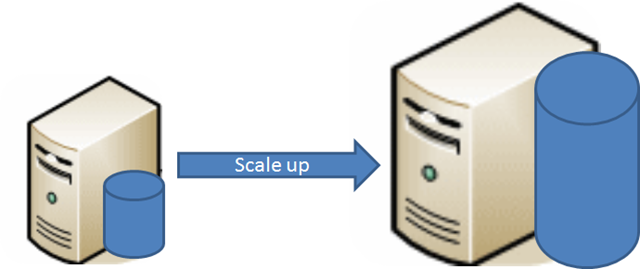
\includegraphics[width=0.5\textwidth]{figuras/cap2/scale_up.png}
	\caption{\textit{Vertical scaling} o \textit{Scaling up} }
	\label{figure:figure_scale_up}
\end{figure}

Entonces tiene sentido  considerar \textit{scaling horizontally} o \textit{scaling out}(\refFigura{figure:figure_scale_out}). En lugar de reforzar un único nodo, \textit{scalling horizontally} significa distribuir la base de datos sobre múltiples maquinas. Dado que \textit{horizontally scaled architecture} puede utilizar \textit{comodity hardware}, el costo de \textit{hosting} el total de los datos puede ser reducido significativamente. Incluso, la distribución  de los datos sobre maquinas mitiga las consecuencias de fallo. Las maquinas inevitablemente fallaran de algún momento a otro. Si se \textit{scaled vertically} , y la maquina falla, entonces es necesario tratar con una falla en un maquina de la cual la mayoría del sistema depende. Podría no considerarse un tema si una copia de los datos existe en un \textit{replicated slave}, pero aun esta el caso en que solo un único \textit{sever} es necesario para bajar el sistema completo. En contraste con el fallo dentro de un \textit{horizontally scaled architecture}. Esto podría ser menos catastrófico dado que una sola máquina representa un porcentaje menor del sistema completo.

\begin{figure}[h!]
	\centering
	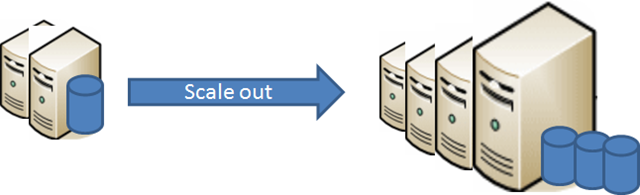
\includegraphics[width=0.5\textwidth]{figuras/cap2/scale_out.png}
	\caption{\textit{Horizontally scaling} o \textit{Scaling out} }
	\label{figure:figure_scale_out}
\end{figure}

\subsubsection{Conclusion}

Es cierto que la mayoría de las bases de datos \gloss{nosql} no fueron construidas considerando \ecommerce. Las bases de datos que carecen modelos de datos enriquecidos, consultas dinámicas, y la noción de \textit{transactionality} no puede esperarse que compitan en el espacio de \ecommerce, entonces no es comprensible que no se considere \mongodb tampoco.

Pero para las partes en donde el sitio \ecommerce comprende el manejo de contenido, \mongodb es claro vencedor. E incluso para mas \textit{transactional components} del sistema, \mongodb tiene características que hacen de la posibilidad de correr un sistema completo de \ecommerce una realidad.


\section{Node.js}

%La craciente popularidad de JavaScript a traiado consigo una gran cantidad de cambios, y la manera en la cual los desarrolladores afrontan el desarrollo \textit{web} es dramaticamente distinto. Las cosas que se pueden hacer en la \textit{web} estos dias con JavaScript Corriendo en el servidor, de la misma manera como en el browser, era dificilmente imaginable hasta hace unos años atras, o fuimos encaptulados dentro de ambientes de \textit{sandbox} como Flash o Java Applets.
%JavaScript’s rising popularity has brought with it a lot of changes, and the face of web development today is dramatically different. The things that we can do on the web nowadays with JavaScript running on the server, as well as in the browser, were hard to imagine just several years ago, or were encapsulated within sandboxed environments like Flash or Java Applets.

%Before digging into Node.js, you might want to read up on the benefits of using JavaScript across the stack which unifies the language and data format (JSON), allowing you to optimally reuse developer resources. As this is more a benefit of JavaScript than Node.js specifically, we won’t discuss it much here. But it’s a key advantage to incorporating Node in your stack.

%As Wikipedia states: “Node.js is a packaged compilation of Google’s V8 JavaScript engine, the libuv platform abstraction layer, and a core library, which is itself primarily written in JavaScript.” Beyond that, it’s worth noting that Ryan Dahl, the creator of Node.js, was aiming to create real-time websites with push capability, “inspired by applications like Gmail”. In Node.js, he gave developers a tool for working in the non-blocking, event-driven I/O paradigm.

%After over 20 years of stateless-web based on the stateless request-response paradigm, we finally have web applications with real-time, two-way connections.

En una frase: Node.js brilla en aplicaciones \textit{web} \textit{real-time} utilizando tecnología \textit{push} sobre \textit{websockets}. Que es tan revolucionario en relación a esto? Después de 20 años de \textit{stateless-web} en el paradigma \textit{request-response} finalmente existen aplicaciones \textit{web} en \textit{real-time}, conexiones \textit{two-way}, donde cliente y servidor pueden iniciar la comunicación, permitiendo intercambiar datos libremente. Esto es un contraste enorme al paradigma típico de \textit{web response}, donde el cliente siempre iniciaba la comunicación. Adicionalmente, esta todo basado en \textit{open web stack} (HTML, CSS y JS )corriendo sobre el \textit{standar port} 80.
%In one sentence: Node.js shines in real-time web applications employing push technology over websockets. What is so revolutionary about that? Well, after over 20 years of stateless-web based on the stateless request-response paradigm, we finally have web applications with real-time, two-way connections, where both the client and server can initiate communication, allowing them to exchange data freely. This is in stark contrast to the typical web response paradigm, where the client always initiates communication. Additionally, it’s all based on the open web stack (HTML, CSS and JS) running over the standard port 80.

Se puede discutir sobre que estas características existían hace años a través de Flash y Java Applets, pero en realidad, esos fueron \textit{sandboxes environment} utilizando la \textit{web} como un protocolo de transporte para entregar al cliente. Ademas, ellos corrían aislados y generalmente sobre \textit{non-standard ports}, los cuales podrían requerir permisos extras.
%One might argue that we’ve had this for years in the form of Flash and Java Applets—but in reality, those were just sandboxed environments using the web as a transport protocol to be delivered to the client. Plus, they were run in isolation and often operated over non-standard ports, which may have required extra permissions and such.

Con todas esta ventajas, Node.js ahora juega un role crítico en el \textit{stack} de tecnología de las principales compañías \textit{high-profile}\cite{online_nodejs_highprofilecompanies} \textbf{las cuales dependen de sus beneficios únicos}.
%With all of its advantages, Node.js now plays a critical role in the technology stack of many high-profile companies who depend on its unique benefits.

%In this post, I’ll discuss not only how these advantages are accomplished, but also why you might want to use Node.js—and why not—using some of the classic web application models as examples.

%How Does It Work?

La principal idea de Node.js : usar \textit{non-blocking}, \textit{event-driven I/O} para permanecer liviano y eficiente para enfrentar aplicaciones \textit{data-intensive} \textit{real-time} que corren a través de dispositivos distribuidos.
%The main idea of Node.js: use non-blocking, event-driven I/O to remain lightweight and efficient in the face of data-intensive real-time applications that run across distributed devices.

%That’s a mouthful.

Lo que esto realmente significa es que Node.js no es una plataforma \textit{panacea} que dominara \textit{web development world}. \textbf{En lugar de eso, es una plataforma que llena una necesidad particular}. Esto es absolutamente esencial. Definitivamente no se deseara utilizar Node.js para operaciones \textit{CPU-intensive}; de hecho, utilizando esto para \textit{heavy computation} anulará practicamente todas sus ventajas. Donde Node.js realmente brilla es \textit{building fast}, aplicaciones \textit{scalable network}, ya que es capaz de manejar un gran número de conexiones simultaneas con un alto rendimiento, lo que equivale a una \textit{high scalability}.
%What it really means is that Node.js is not a silver-bullet new platform that will dominate the web development world. Instead, it’s a platform that fills a particular need. And understanding this is absolutely essential. You definitely don’t want to use Node.js for CPU-intensive operations; in fact, using it for heavy computation will annul nearly all of its advantages. Where Node really shines is in building fast, scalable network applications, as it’s capable of handling a huge number of simultaneous connections with high throughput, which equates to high scalability.

Como trabaja \textit{under-the-hood} es muy interesante. Comparado con la técnica tradicional \textit{web-serving} donde cada conexión (\textit{request}) engendra un nuevo \textit{thread}, ocupando memoria \gloss{memory_ram} del sistema y, eventualmente \textit{maxing-out} la cantidad de \gloss{memory_ram} disponible, Node.js opera en un \textit{single-thread}, usando llamadas \textit{non-blocking I/O}, permitiendo el apoyo de decenas de miles de conexiones concurrentes (retenidas en el \textit{event loop}). \refFigura{figure:diagram_traditional_vs_nodejs_server_thread}.
%How it works under-the-hood is pretty interesting. Compared to traditional web-serving techniques where each connection (request) spawns a new thread, taking up system RAM and eventually maxing-out at the amount of RAM available, Node.js operates on a single-thread, using non-blocking I/O calls, allowing it to support tens of thousands of concurrent connections (held in the event loop).


\begin{figure}[h!]
	\centering
	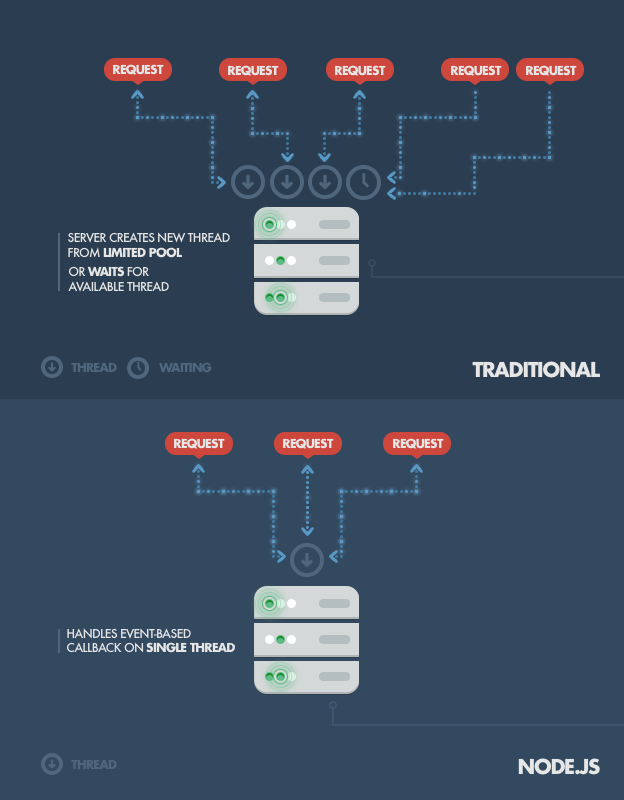
\includegraphics[width=0.5\textwidth]{figuras/cap2/diagram_traditional_vs_node_serverthread.png}
	\caption{Diagrama de \textit{Traditional} vs. Node.js \textit{server thread}}
	\label{figure:diagram_traditional_vs_nodejs_server_thread}
\end{figure}



Un cálculo rápido: asumiendo que cada \textit{thread} potencialmente tiene asignado 2 MB de memoria con ella, corriendo en un sistema con 8 GB de \gloss{memory_ram} nos coloca en un teórico máximo de 4000 conexiones concurrentes, ademas del costo por cambio de contexto entre \textit{threads}. Ese es el escenario el cual tipicamente se encuentran técnicas tradicionales de \textit{web-serving}. Evitando todo eso, Node.js logra niveles de \textit{scalability} sobre 1M de conexiones concurrentes (como \textit{proof-of-concept}).
%A quick calculation: assuming that each thread potentially has an accompanying 2 MB of memory with it, running on a system with 8 GB of RAM puts us at a theoretical maximum of 4000 concurrent connections, plus the cost of context-switching between threads. That’s the scenario you typically deal with in traditional web-serving techniques. By avoiding all that, Node.js achieves scalability levels of over 1M concurrent connections (as a proof-of-concept).

Hay, por supuesto, la cuestión de compartir un solo \textit{thread} entre todos los \textit{request} de clientes, y es una potencial trampa de escribir aplicaciones Node.js. Primeramente, \textit{heavy computation} puede asfixiar el único \textit{thread} de Node.js y causar problemas en todos los clientes como \textit{incoming request} podrían ser bloqueados hasta que dicho \textit{computation} sea completado. En segundo lugar, desarrolladores necesitan ser realmente cuidadosos en no permitir que una excepción \textit{bubbling up} al \textit{core} del \textit{event loop} de Node.js, el cual puede causar que la instancia Node.js termine (efectivamente \textit{crashing} el programa).
%There is, of course, the question of sharing a single thread between all clients requests, and it is a potential pitfall of writing Node.js applications. Firstly, heavy computation could choke up Node’s single thread and cause problems for all clients (more on this later) as incoming requests would be blocked until said computation was completed. Secondly, developers need to be really careful not to allow an exception bubbling up to the core (topmost) Node.js event loop, which will cause the Node.js instance to terminate (effectively crashing the program).

La técnica utilizada para evitar excepciones \textit{bubbling up to the surface} es pasando el error de regreso al \textit{caller} como parámetro de \textit{callback} (en lugar de lanzarlos, como en otros ambientes). Incluso si alguna excepción no controlada conduce a \textit{bubble up}, hay múltiples paradigmas y herramientas disponibles para monitorear el proceso Node y realizar lo necesario para recuperarse de un \textit{crashed instance} (aunque no este disponible para recuperar sesiones de usuarios), siendo el mas común el módulo Forever\cite{online_github_nodejitsu_forever}.
%The technique used to avoid exceptions bubbling up to the surface is passing errors back to the caller as callback parameters (instead of throwing them, like in other environments). Even if some unhandled exception manages to bubble up, there are mutiple paradigms and tools available to monitor the Node process and perform the necessary recovery of a crashed instance (although you won’t be able to recover users’ sessions), the most common being the Forever module, or a different approach with external system tools upstart and monit.

%NPM: The Node Package Manager

%When discussing Node.js, one thing that definitely should not be omitted is built-in support for package management using the NPM tool that comes by default with every Node.js installation. The idea of NPM modules is quite similar to that of Ruby Gems: a set of publicly available, reusable components, available through easy installation via an online repository, with version and dependency management.

%A full list of packaged modules can be found on the NPM website https://npmjs.org/ , or accessed using the NPM CLI tool that automatically gets installed with Node.js. The module ecosystem is open to all, and anyone can publish their own module that will be listed in the NPM repository. A brief introduction to NPM (a bit old, but still valid) can be found at http://howtonode.org/introduction-to-npm.

%Some of the most popular NPM modules today are:

%express - Express.js, a Sinatra-inspired web development framework for Node.js, and the de-facto standard for the majority of Node.js applications out there today.
%connect - Connect is an extensible HTTP server framework for Node.js, providing a collection of high performance “plugins” known as middleware; serves as a base foundation for Express.

%socket.io and sockjs - Server-side component of the two most common websockets components out there today.

%Jade - One of the popular templating engines, inspired by HAML, a default in Express.js.

%mongo and mongojs - MongoDB wrappers to provide the API for MongoDB object databases in Node.js.

%redis - Redis client library.
%coffee-script - CoffeeScript compiler that allows developers to write their Node.js programs using Coffee.
%underscore (lodash, lazy) - The most popular utility library in JavaScript, packaged to be used with Node.js, as well as its two counterparts, which promise better performance by taking a slightly different implementation approach.
%forever - Probably the most common utility for ensuring that a given node script runs continuously. Keeps your Node.js process up in production in the face of any unexpected failures.
%The list goes on. There are tons of really useful packages out there, available to all (no offense to those that I’ve omitted here).

%Examples of Where Node.js Should Be Used


%Where Node.js Can Be Used

%SERVER-SIDE WEB APPLICATIONS

%Node.js with Express.js can also be used to create classic web applications on the server-side. However, while possible, this request-response paradigm in which Node.js would be carrying around rendered HTML is not the most typical use-case. There are arguments to be made for and against this approach. Here are some facts to consider:

%Pros:

%If your application doesn’t have any CPU intensive computation, you can build it in Javascript top-to-bottom, even down to the database level if you use JSON storage Object DB like MongoDB. This eases development (including hiring) significantly.
%Crawlers receive a fully-rendered HTML response, which is far more SEO-friendly than, say, a Single Page Application or a websockets app run on top of Node.js.
%Cons:

%Any CPU intensive computation will block Node.js responsiveness, so a threaded platform is a better approach. Alternatively, you could try scaling out the computation [*].
%Using Node.js with a relational database is still quite a pain (see below for more detail). Do yourself a favour and pick up any other environment like Rails, Django, or ASP.Net MVC if you’re trying to perform relational operations.
%[*] An alternative to these CPU intensive computations is to create a highly scalable MQ-backed environment with back-end processing to keep Node as a front-facing ‘clerk’ to handle client requests asynchronously.
%Where Node.js Shouldn’t Be Used
%
%SERVER-SIDE WEB APPLICATION W/ A RELATIONAL DB BEHIND
%
%Comparing Node.js with Express.js against Ruby on Rails, for example, there is a clean decision in favour of the latter when it comes to relational data access.
%
%Relational DB tools for Node.js are still in their early stages; they’re rather immature and not as pleasant to work with. On the other hand, Rails automagically provides data access setup right out of the box together with DB schema migrations support tools and other Gems (pun intended). Rails and its peer frameworks have mature and proven Active Record or Data Mapper data access layer implementations, which you’ll sorely miss if you try to replicate them in pure JavaScript.[*]
%
%Still, if you’re really inclined to remain JS all-the-way (and ready to pull out some of your hair), keep an eye on Sequelize and Node ORM2—both are still immature, but they may eventually catch up.
%
%[*] It’s possible and not uncommon to use Node solely as a front-end, while keeping your Rails back-end and its easy-access to a relational DB.
%HEAVY SERVER-SIDE COMPUTATION/PROCESSING
%
%When it comes to heavy computation, Node.js is not the best platform around. No, you definitely don’t want to build a Fibonacci computation server in Node.js. In general, any CPU intensive operation annuls all the throughput benefits Node offers with its event-driven, non-blocking I/O model because any incoming requests will be blocked while the thread is occupied with your number-crunching.
%
%As stated previously, Node.js is single-threaded and uses only a single CPU core. When it comes to adding concurrency on a multi-core server, there is some work being done by the Node core team in the form of a cluster module [ref: http://nodejs.org/api/cluster.html]. You can also run several Node.js server instances pretty easily behind a reverse proxy via nginx.
%
%With clustering, you should still offload all heavy computation to background processes written in a more appropriate environment for that, and having them communicate via a message queue server like RabbitMQ.
%
%Even though your background processing might be run on the same server initially, such an approach has the potential for very high scalability. Those background processing services could be easily distributed out to separate worker servers without the need to configure the loads of front-facing web servers.
%
%Of course, you’d use the same approach on other platforms too, but with Node.js you get that high reqs/sec throughput we’ve talked about, as each request is a small task handled very quickly and efficiently.
%
%Conclusion
%
%We’ve discussed Node.js from theory to practice, beginning with its goals and ambitions, and ending with its sweet spots and pitfalls. When people run into problems with Node, it almost always boils down to the fact that blocking operations are the root of all evil—99% of Node misuses come as a direct consequence.
%
%In Node, blocking operations are the root of all evil—99% of Node misuses come as a direct consequence.
%
%Remember: Node.js was never created to solve the compute scaling problem. It was created to solve the I/O scaling problem, which it does really well.

%Why use Node.js? If your use case does not contain CPU intensive operations nor access any blocking resources, you can exploit the benefits of Node.js and enjoy fast and scalable network applications. Welcome to the real-time web.

\subsection{Desempeño de Node.js frente a sus competidores}
	A continuación se realizan comparaciones en el desempeño de la plataforma  con algunos de sus símiles mas conocidos los cuales corresponden a:
	
	\begin{itemize}
		\item Java
		\item Ruby
		\item PHP
	\end{itemize}

\subsubsection{Node.js vs Java \cite{online_nodejs_paypal}}



La primera adopción que hizo Paypal con Node.js no fue una aplicación menor; esto fue su \textit{account overview page} y una de las mas \textit{trafficked} \textit{apps} en el \textit{website}. Ellos tomaron un gran riesgo, pero lo hicieron con la finalidad de determinar si realmente la nueva plataforma representaba una mejora con respecto al sistema actual.
%Our first adopter of node.js in production wasn’t a minor application; it was our account overview page and one of the most trafficked apps on the website. We decided to go big, but we also mitigated that risk by building the equivalent Java application in parallel. We knew how to deploy and scale Java applications, so if anything went wrong with the node.js app, we could fall back to the Java one. This provided the setting for some interesting data.

Una vez que la aplicación con \nodejs logro las mismas funcionalidades que la aplicación actual, persivieron el siguiente resultado:

\begin{itemize}
\item Fue construida casi \textbf{el doble de rápido con menos personal}.
\item Escrito con un \textbf{33\% menos de lineas de código}.
\item Construida con \textbf{40\% menos de archivos}.
\end{itemize}

Por si solo, esta evidencia mostraba a los equipos desarrollar más rápido utilizando \javascript.

\performance fue un tópico interesante. Se pudo analizar 2 aplicaciones con exactamente las mismas funcionalidades: una con \framework Java interno basado en Spring y la otra construida en \textit{kraken.js} usando Express, dust.js y otros códigos \opensource.
%Performance is a fun and debatable topic. In our case, we had two applications with the exact same functionality and built by roughly the same teams: one on our internal Java framework based on Spring and the other built on kraken.js using express, dust.js and other open source code.

Se ejecutaron los test adecuados utilizando \hardware de producción que probaran las rutas y recolectaran datos de rendimiento y tiempo de respuesta. Los resultados se aprecian en \refFigura{figure:java_benchmark_paypal}.
%We ran our test suite using production hardware that tested the routes and collected data on throughput and response time.

\begin{figure}[h!]
	\centering
	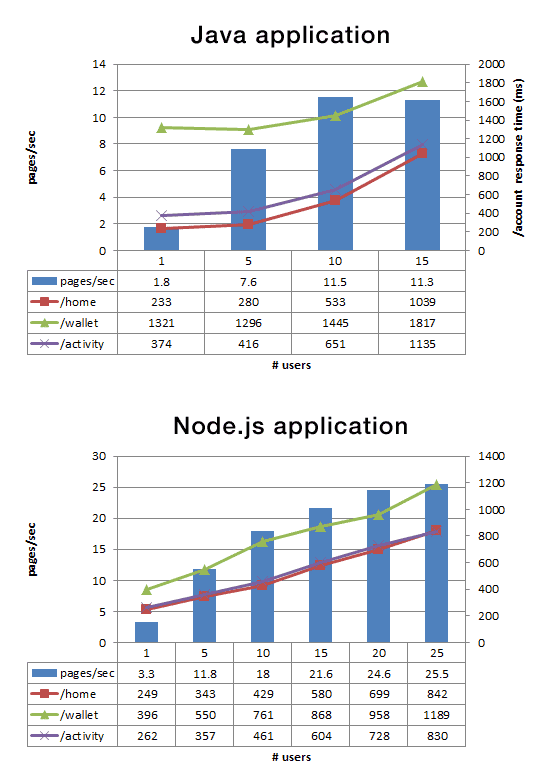
\includegraphics[width=0.6\textwidth]{figuras/cap2/java_nodejs_benchmark_paypal.png}
	\caption{\textit{Performance} de la aplicación en Java y Node.js}
	\label{figure:java_benchmark_paypal}
\end{figure}

Se observa que la aplicación utilizando Node.js tiene:
%You can see that the node.js application had:

\begin{itemize}
\item El doble de solicitudes por segundo vs. la aplicación Java. Esto es incluso mas interesante porque los resultados iniciales de rendimiento estaban utilizando un solo núcleo para la aplicación \nodejs, en comparación con cinco núcleos en Java. Esperan aumentar aun más esta brecha en el futuro.
%Double the requests per second vs. the Java application. This is even more interesting because our initial performance results were using a single core for the node.js application compared to five cores in Java. We expect to increase this divide further.
\item \textbf{Disminución en un 35\% en el tiempo promedio de respuesta} para la misma página. Esto resulto ser \textbf{200ms mas rápido} en el servidor. Algo que los usuarios definitivamente notan.
%35% decrease in the average response time for the same page. This resulted in the pages being served 200ms faster— something users will definitely notice.
\end{itemize}

%There’s a disclaimer attached to this data: this is with our frameworks and two of our applications. It’s just about as apples-to-apples a performance test as we could get between technologies, but your milage may vary. That said, we’re excited by what we’ve seen from node.js’ raw performance.

Mas ejemplos de \benchmark pueden ser encontrados en\cite{online_nodejs_java_dzone}.


\subsubsection{Node.js vs PHP\cite{online_nodejs_php_loadimpact}}

No es justo comparar Node.js con PHP. Lo que realmente se compara es \nodejs y PHP+Apacha2 ( u otro servidor http ). Es este caso particular, las pruebas fueron realizadas usando Apache2 y \textit{mod\_php}, dado que es por lejos la configuración mas común. 
%So no, it’s not fair to say that we compare Node.js and PHP. What we really compare is Node.js and PHP+Apache2 (or any other http server). For this article, I’ve used Apache2 and mod_php since it’s by far the most common configuration. Some might say that I’d get much better results if I had used Nginx or Lighthttpd as the http server for PHP. That’s most likely very true, but at the end of the day, server side PHP depends on running in multiple separate processes. Regardless if we create those processes with mod_php or fastcgi or any other mechanism. So, I’m sticking with the standard server setup for PHP and I think that makes good sense.

\begin{figure}[h!]
	\centering
	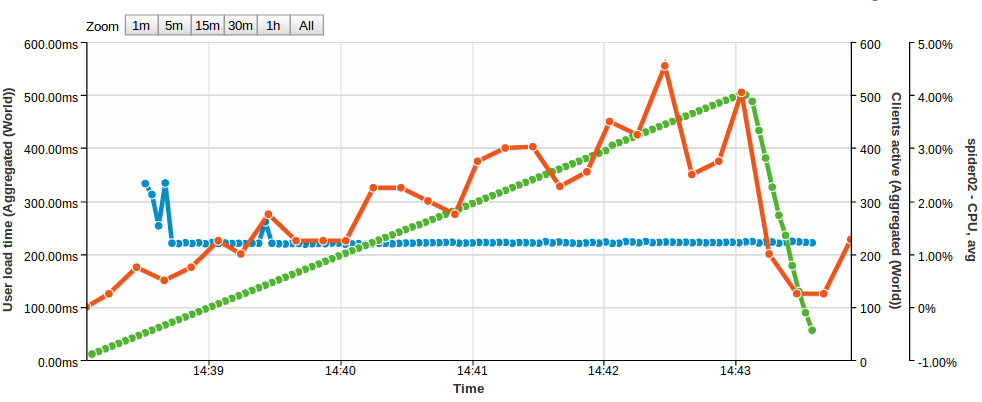
\includegraphics[width=0.6\textwidth]{figuras/cap2/node_benchmak_loadimpact.png}
	\caption{\textit{Performance} de la aplicación Node.js}
	\label{figure:node_benchmark_nodephp}
\end{figure}

El gráfico de \refFigura{figure:node_benchmark_nodephp} muestra lo que sucede cuando se carga el test en el servidor utilizando \nodejs. La respuesta de tiempo (azul) es mucho mas constante durante todo el test. 

%The first graph here shows what happens when we load test the Node.js server. The response time (blue) is pretty much constant all through the test. My back of a napkin analysis of the initial outliers is that they have to do with a cold MySQL cache. Now, have a look at the results from the PHP test:


\begin{figure}[h!]
	\centering
	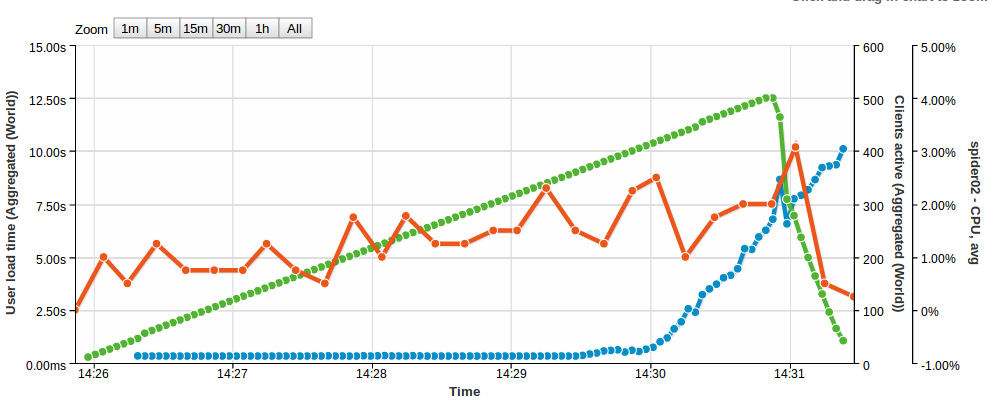
\includegraphics[width=0.6\textwidth]{figuras/cap2/phpapache_benchmak_loadimpact.png}
	\caption{\textit{Performance} de la aplicación en PHP/Apache}
	\label{figure:php_benchmark_nodephp}
\end{figure}

Muy diferente los resultados para el caso de \php(\refFigura{figure:php_benchmark_nodephp}). No es sencillo observar que sucede, pero las lineas azules están inicialmente estables a 320ms hasta cerca de 340 usuarios activos simultáneos. Después de eso, se observa un pequeño incremento en el tiempo de respuesta pero después de agregar mas usuarios activos simultáneos, el tiempo de respuesta se dispara por completo. 
%Quite different results. It’s not easy to see on this screen shot, but the blue lines is initially stable at 320 ms response time up to about 340 active concurrent users. After that, we first see a small increase in response time but after additional active concurrent users are added, the response time eventually goes through the roof completely.

¿ Qué problema tiene \php/Apache?
%So what’s wrong with PHP/Apache?

La diferencia no es de sorprender. Esto es producto de la diferencia de arquitectura entre ambas soluciones.
%Ok, so what we’re looking at is not very surprising, it’s the difference in architecture between the two solutions. Let’s think about what goes on in each case.

Cuando Apache2 sirve a una pagina PHP, este deja la ejecución \php a un \textit{child process} específico. Ese \textit{child process} puede solo manejar una solicitud \php al mismo tiempo, así que si hay mas solicitudes, las otras deben esperar. En el servidor hay un máximo de 256 clientes (\textit{MaxClients}) configurados vs 150 que vienen por defecto. Incluso si es posible aumentar el \textit{MaxClients} hasta mas allá de 256, habrá problemas con la memoria interna(\gloss{memory_ram}), Al final, se necesita encontrar el balance correcto entre el máximo numero de solicitudes simultaneas y los recursos disponibles del servidor.
%When Apache2 serves up the PHP page it leaves the PHP execution to a specific child process. That child process can only handle one PHP request at a time so if there are more requests than than, the others have to wait. On this server, there’s a maximum of 256 clients (MaxClients) configured vs 150 that comes standard. Even if it’s possible to increase MaxClients to well beyond 256, that will in turn give you a problem with internal memory (RAM). At the end, you need to find the correct balance between max nr of concurrent requests and available server resources.

Pero para Node.js, es sencillo. Después de todo, cada solicitud es cerca de 30\% mas rápido que \php, así que en \performance, el cual es una configuración extremadamente básica, \nodejs es mas rápido. Ademas, en Node.js Todo esta en un solo proceso en el servidor. Un proceso manejando una solicitud activa. Así que no existe una comunicación interna de procesos entre diferentes instancias y el proceso madre. Incluso, pos solicitud, \nodejs es mucho mas eficiente. \php/Apache necesita muchísimo \php y sobrecarga de procesos por cada concurrente \textit{worker/client} mientras \nodejs compartirá la mayoría de su memoria entre las solicitudes.
%But for Node, it’s easier. First of all, in the calm territory, each request is about 30% faster than for PHP, so in pure performance in this extremely basic setup, Node is quicker. Also going for Node is the fact that everything is in one single process on the server. One process with one active request handling thread. So thre’s no inter process communication between different instances and the ‘mother’ process. Also, per request, Node is much more memory efficient. PHP/Apache needs to have a lot of php and process overhead per concurrent worker/client while Node will share most of it’s memory between the requests.

%Also note that in both these tests, CPU load was never a problem. Even if CPU loads varies with concurrent users in both tests it stays below 5% (and yes, I did not just rely on the graph, I checked it on the server as well). (I’ll write a follow up on this article at some point when I can include server memory usage as well). So we haven’t loaded this server into oblivion in any way, we’ve just loaded it hard enough for the PHP/Aapache architecture to start showing some of it’s problems.

Mas ejemplos de \textit{benchmark} pueden ser encontrados en\cite{online_nodejs_java_appdynamics}.


%\subsubsection*{¿ Qué hace a Node.js mejor?}
%
%Node.js introduce al menos 2 nuevas características ( para una amplia audiencia ). Primero, la habilidad  de escribir código JavaScript en el lado del servidor. En teoría esto puede ser una ventaja dado que JavaScipt es mas importante que nunca en el lado del cliente y usando el mismo lenguaje en el servidor y en el navegador deberían haber muchísimos beneficios. 
%%Node.js introduces at least two new things (for a broader audience). First, the ability to write server side JavaScript code. In theory this could be an advantage since JavaScript is more important than ever on the client side and using the same language on server and browser would have many benefits. That’s at least quite cool.
%
%La otra cosa que introduce Node.js es que es completamente asíncrono y orientado al evento. Node.js esta basado en el supuesto que muchísimo código de computador realmente espera por I/O la mayoría del tiempo, como esperando por un archivo para ser escrito en el disco o por una solicitud MySQL para retornar \textit{data}. Para lograr eso, mas o menos cada función en Node.js es \textit{non-blocking}.
%%The other thing that makes Node.js different is that it’s completely asynchronous and event driven. Node is based on the realization that a lot of computer code actually just sits idle and wait for I/O most of the time, like waiting for a file to be written to disk or for a MySQL query to return data. To accomplish that, more or less every single function in Node.js is non-blocking.
%
%Cuando se solicita a nodo abrir un archivo, no se espera a que retorne. En lugar de eso, se le comunica a Node.js a que función se le entrega el resultado y continuar con otra ejecución. Esto conduce a una dramática diferencia  para estructurar el código con \textit{callback} anidados y funciones anónimas de clausura.  Terminaras con algo como esto:
%%When you ask for node to open a file, you don’t wait for it to return. Instead, you tell node what function to pass the results to and get on with executing other statements. This leads to a dramatically different way to structure your code with deeply nested callbacks and anonymous function and closures. You end up with something  like this:
%
%
%\medskip
%\begin{lstlisting}[caption= Ejemplo de anidación de funciones.]
%	doSomething(val, function(err,result){
%		doSomethingElse(result,function(err,res){
%			doAbra();
%			doKadabra(err, res, function() {
%				...
%				...
%			});
%		});
%	});
%\end{lstlisting}
%
%
%La cualidad que hace diferente a Node.js, es que no es necesario utilizar un servidor http(s) separado. Es completamente común poner Node.js detrás de un Nginx, pero eso no es estrictamente necesario. Así que el corazón de las aplicaciones \textit{web} típicas de Node.js  es la implementación de su servidor real.
%It’s quite easy to end up with very deep nesting that in my opinion sometimes affects code readability in a negative way. But compared to what gets said about PHP, that’s very mild critique. And.. oh! The third thing that is quite different is that in Node.js, you don’t have to use a separate http(s) server. It’s quite common to put Node.js behind a Nginx, but that’s not strictly needed. So the heart of a typical Node.js web application is the implementation of the actual web server.


*****************************************************************************


Hopefully, this shows the inherit differences in two different server technologies. One old trusted and one young and trending. Hopefully it’s apparent that your core technical choices will affect your server performance and in the end, how much load you can take. Designing for high load and high scalability begins early in the process, before the first line of code is ever written.

And sure, in real life, there are numerous of tricks available to reduce the effects seen here. In real life, lots of Facebook still runs on PHP.


\subsubsection{Node.js y \ecommerce}

\ecommerce es un excelente ejemplo de sistema que se puede ver totalmente beneficiado con el uso de Node en el lado del servidor. 

\begin{itemize}
	\item \textbf{\frontend se movió desde el \serverside al \clientside( al menos en \mobile )}. Una de las grandes consecuencias es que el server-side ya no es mas CPU Bound ahora es Memory Bound e I/O Bound. \nodejs es \textit{event-driven}, lo cual implica eficiencia en I/O Bound y es extremadamente eficiente en el uso de memoria.
	\item Permite velocidad de desarrollo y ejecución. En otras palabras iteraciones rápidas.
	%Ease of Development-Some problem, somewhere has a solution best written in Brainf*ck. But implementing that solution (in Brainfuck) will be nearly impossible to write, let alone read. It will cost you time and a tremendous amount of effort. In general, you should use languages and platform that make development easier, not harder for you (or anyone that might work on it later).
	\item \textbf{Comunidad}: Existe una activa comunidad la cual esta constantemente solucionando dudas, ademas de proporcionar módulos para resolver problemas conocidos.
	\item \textbf{Reutilizar código}: \serverside y \clientside usan el mismo lenguaje, permitiendo reutilización de componentes.
	\item \textbf{Optimiza el uso de recursos}: Los desarolladores de \clientside pueden desarrollar en \serverside, ya que son el mismo lenguaje.
	\item \textbf{Scalability}: Los sitios \textit{web} se encuentran en constante crecimiento. \textit{Scalability} es una consecuencia de la eficiencia que tiene \nodejs para Memory Bound e I/O Bound
\end{itemize}

%+++++++++++++++++++++++++++++++++++++++++++++++++++++++++++++++++++++++
%
%
%Node no es la panacea para todo, tiene muchos issues con los cuales hay que lidiar, pero es probable una de las mejores soluciones que se pueden tomar(LinkedIn).
%
%***************************************************************************
%Kiran Prasad, Sr. Director, Mobile Engineering, LinkedIn
%
%Una pregunta interesante saber cuales son los problemas que te hicieron mirar hacia nodeJ(pregunta a KIRAN Prased)
%
%Cuando llegue a LinkedIN estabamos corriendo cosas en Ruby and Rails stack, una de las cosas que encontramos es que el FRONT-END se movio desde el server-side al client-side( al menos en mobile ). Ese gran shift cambio  las necesidades del front-end y el server-side.
%
%El server-side ya no es mas CPU Bound ahora es Memory Bound e I/O Bound
%
%Nodejs run de forma muy eficiente en I/O 
%
%Dio velocidad de desarrollo, de ejecución, iteraciónes mas rápidas 
%
%Este tipo de razones nos mostrarón la necesidad de I/O Bound necesitan ser I/O event
%Necesitaban eficiencia de memoria, y Node es super eficiente en ese sentido.
%La convinación de estos elementos  
%
%eficiencia en memoria
%
%
%
%***************************************************************************
%Sri Viswanath, SVP Engineering and Operations, Groupon
%
%
%
%Need low latency
%
%
%
%***************************************************************************
%Jigar Desai, Sr. Director, Platforms, eBay
%
%
%
%
%
%
%***************************************************************************
Billy Scott, PayPal

\section{\textit{Client side}}

Elegir el \framework correcto para un proyecto puede tener un impacto tremendo en la habilidad de entregar a tiempo y la habilidad para mantener el código en el futuro. ES ciertamente deseable un \framework solido, estable y probado, pero sin estar limitado por la opción. La \web entra evolucionando rápidamente; nuevas tecnologías surgen, y metodologías antiguas rápidamente se vuelven irrelevantes. Bajo este escenario, se compararan 3 \frameworks.
%In this article we are going to compare three popular MV* frameworks for the web: AngularJS vs. Backbone vs. Ember. Choosing the right framework for your project can have a huge impact on your ability to deliver on time, and your ability to maintain your code in the future. You probably want a solid, stable and proven framework to build upon, but don't want to be limited by your choice. The web is evolving fast — new technologies arise, and old methodologies quickly become irrelevant. Under this light, we are going to go through an in-depth comparison of the three frameworks.

\subsection{Meet The \frameworks}

%All the frameworks we are going to meet today have a lot in common: they are open-sourced, released under the permissive MIT license, and try to solve the problem of creating Single Page Web Applications using the MV* design pattern. They all have the concept of views, events, data models and routing. We are going to start with some quick background and history, and then dive in to compare the three frameworks.
%
%AngularJS was born in 2009 as a part of a larger commercial product, called GetAngular. Shortly after, Misko Hevery, one of the engineers who founded GetAngular, managed to recreate a web application that consisted of 17 thousand lines of code and took 6 months to develop in a mere 3 weeks using just GetAngular. Reducing the size of the application to just about 1,000 lines of code convinced Google to start sponsoring the project, turning it into the open-source AngularJS we know today. Amongst Angular's unique and innovative features are two-way data bindings, dependency injection, easy-to-test code and extending the HTML dialect by using directives.
%
%Backbone.js is a lightweight MVC framework. Born in 2010, it quickly grew popular as a lean alternative to heavy, full-featured MVC frameworks such as ExtJS. This resulted in many services adopting it, including Pinterest, Flixster, AirBNB and others.
%
%Ember's roots go way back to 2007. Starting its life as the SproutCore MVC framework, originally developed by SproutIt and later by Apple, it was forked in 2011 by Yehuda Katz, a core contributor to the popular jQuery and Ruby on Rails projects. Notable Ember users include Yahoo!, Groupon, and ZenDesk.

\subsection{Comunidad}

Una comunidad es uno de los factores mas importantes para considerar cuando se elije un \textit{framework}. Una extensa comunidad significa mas preguntas contestadas, mas módulos \textit{third-party}, mas tutoriales en youtube, etc. Angular es sin dudas la plataforma con mas apoyo como se puede observar en \reftabla{tab:framework_community}.
%Community is one of the most important factors to consider when choosing a framework. A large community means more questions answered, more third-party modules, more YouTube tutorials…you get the point. I have put together a table with the numbers, as of August 16, 2014. Angular is definitely the winner here, being the 6th most-starred project on GitHub and having more questions on StackOverflow than Ember and Backbone combined, as you can see below:
%
%
\begin{table}[h!]
    \tiny
   
%\begin{tabular}{ |C{0.3\paperwidth}|C{0.3\paperwidth}| }
\begin{tabular}{ |L{0.1\paperwidth}|L{0.2\paperwidth}|L{0.2\paperwidth}|L{0.2\paperwidth}|}
\hline
	Metric&
	AngularJS &
	Backbone.js &
	Ember.js
	
\\ \hline
	Stars on Github&
	27.2k&
	18.8k&
	11k
	
\\ \hline
	Third-Party Modules&
	800 ngmodules&
	236 backplugs&
	21 emberaddons
	
\\ \hline
	StackOverflow Questions&
	49.5k&
	15.9k&
	11.2k
	
\\ \hline
	YouTube Results&
	~75k&
	~16k&
	~6k
	
\\ \hline
	GitHub Contributors&
	928&
	230&
	393
	
\\ \hline
	Chrome Extension Users&
	150k&
	7k&
	38.3k
				
\\ \hline
\end{tabular}
    \caption{ Tamaño de la comunidad}
    \label{tab:framework_community}
\end{table}
%Metric	AngularJS	Backbone.js	Ember.js
%Stars on Github	27.2k	18.8k	11k
%Third-Party Modules	800 ngmodules	236 backplugs	21 emberaddons
%StackOverflow Questions	49.5k	15.9k	11.2k
%YouTube Results	~75k	~16k	~6k
%GitHub Contributors	928	230	393
%Chrome Extension Users	150k	7k	38.3k

%TODO
%Todas las medidas, sin embargo, muestran simplemente el estado actual de cada \textit{framework}. También es interesante de observar cual \textit{framework} tienen el mayor crecimiento de popularidad. 
%All those metrics, however, merely show the current state of each framework. It is also interesting to see which framework has a faster-growing popularity. Fortunately, using Google Trends we can get an answer for that too:


\subsection{Framework Size}

El tiempo de carga para las paginas es crucial para el éxito de un sitio \textit{web}. Los usuarios no muestran mucha paciencia cuando se trata de la velocidad de explorar; así que en muchos casos es deseado hacer todo lo posible para carga la aplicación tan rápido como sea posible. Hay 2 factores para observar que deben considerarse para el impacto del \textit{framework} en el tiempo de carga de la aplicación: el tamaño del \textit{framework} y el tiempo que le toma al \textit{framework} \textit{bootstrap}.
%Page load times are crucial for the success of your web site. Users do not exhibit much patience when it comes to the speed of browsing — so in many cases it is desired to do everything possible to make your application load as fast as possible. There are two factors to look at when considering the impact of the framework on the loading time of your application: framework size and the time it takes the framework to bootstrap.

Los \textit{assets} de JavaScript son usualmente served \textit{minified} y \textit{gzipped}, asi que se comparará el tamaño de las versiones \textit{minified-gzipped}. Sin embargo, simplemente mirando el \textit{framework} no es suficiente. En \reftabla{tab:framework_size} se aprecia el tamaño de cada \textit{framework}.
%Javascript assets are usually served minified and gzipped, so we are going to compare the size of the minified-gzipped versions. However, merely looking at the framework is not enough. Backbone.js, despite being the smallest (only 6.5kb), requires both Underscore.js (5kb) and jQuery (32kb) or Zepto (9.1kb), and you will probably need to add some third party plug-ins to the mix.

\begin{table}[h!]
    \tiny
\begin{tabular}{ |L{0.1\paperwidth}|L{0.2\paperwidth}|L{0.2\paperwidth}|L{0.2\paperwidth}|}
\hline
	\textit{Framework}&
	Versión &
	Net Size &
	Size with required dependencies
	
\\ \hline
	AngularJS&
	1.2.22&
	39.5kb&
	39.5kb
\\ \hline
	Backbone.js&
	1.1.2&
	6.5kb&
	43.5kb (jQuery + Underscore) 20.6kb (Zepto + Underscore)
	
\\ \hline
	Ember.js&
	1.6.1&
	90kb&
	136.2kb (jQuery + Handlebars)
	
\\ \hline
\end{tabular}
    \caption{ Tamaño del \textit{framework}}
    \label{tab:framework_size}
\end{table}


\section{Full-Stack \gloss{javascript}}
%TODO
%Es importante destacar los beneficios de utilizar \gloss{javascript} a través del \textit{stack} que unifica el lenguaje y el formato de la información (\gloss{json}), permitiendo optimamente reutilizar recursos de desarrollador. 

Programando 
%Before digging into Node.js, you might want to read up on the benefits of using JavaScript across the stack which unifies the language and data format (JSON), allowing you to optimally reuse developer resources. As this is more a benefit of JavaScript than Node.js specifically, we won’t discuss it much here. But it’s a key advantage to incorporating Node in your stack.

Hay una gran cantidad de ventajas al utilizar un único lenguaje a lo largo del \textit{stack}. Al programas con \gloss{javascript} existe la posibildiad de realizar mejoras de rendimiento tanto en el propio \textit{software} y en la productividad de los desarrolladores. Con \gloss{mongodb}, se puede guardar los documentos en un formato \textit{\gloss{json}-like}, escribir consultas \gloss{json} en los servidores basados en ExpressJS y NodeJS, y similarmente pasar documentos \gloss{json} al \textit{front-end} AngularJS. \textit{Debugging} y la administración de la base de datos se vuelve una tarea muchísimo mas sencilla cuando los objetos guardados en la base de datos son esencialmente idénticos a los objetos que el cliente \gloss{javascript} ve. Incluso mejor, alguien trabajando en el lado del cliente puede fácilmente entender el código del lado del servidor y las consultas a la base de datos; usando la misma sintaxis y objetos todo el proceso libera a los desarrolladores la consideración de varios conjuntos de buenas prácticas de lenguajes y reduce la barrera de entrada para la comprensión de su código base. Esto es especialmente importante en una \textit{hackathon}: el equipo puede no tener mucha experiencia trabajando juntos, y con tan poco tiempo para integrar todas las piezas de su proyecto, cualquier detalle que haga el proceso de desarrollo mas sencillo es oro.
%First of all, there are huge advantages to using a uniform language throughout your stack. My team uses a set of tools that we affectionately call the MEAN stack:­ MongoDB, ExpressJS, AngularJS, and Node.js. By coding with Javascript throughout, we are able to realize performance gains in both the software itself and in the productivity of our developers. With MongoDB, we can store our documents in a JSON-­like format, write JSON queries on our ExpressJS and NodeJS based server, and seamlessly pass JSON documents to our AngularJS frontend. Debugging and database administration become a lot easier when the objects stored in your database are essentially identical to the objects your client Javascript sees. Even better, somebody working on the client side can easily understand the server side code and database queries; using the same syntax and objects the whole way through frees you from having to consider multiple sets of language best practices and reduces the barrier to entry for understanding your codebase. This is especially important in a hackathon setting: the team may not have much experience working together, and with such little time to integrate all the pieces of your project, anything that makes the development process easier is gold.


\section{Resumen}
%TODO
Recapitulando, he demostrado que las soluciones actuales de \ecommerce pueden ser considerablemente mejoradas utilizando la tecnología actualmente presente. 
Importante notar que solo estoy ofreciendo una mejor solución a lo que ya existe, en ningún caso indico la solución que presento es la mejor posible. No se ha realizado un estudio sobre todas las opciones disponibles del mercado. Sin embargo esta solución ofrece

speed
scalability
flexibility
performance

%%%%%%%%%%%%%%%%%%%%%%
%								%
%	CONCLUSIONES					%
%								%
%%%%%%%%%%%%%%%%%%%%%

\chapter{Conclusiones} \label{cap:conclusiones}

\section{Trabajos Futuros} \label{cap:conclusiones:trabajos_futuros}

%%%%%%%%%%%%%%%%%%%%%%
%								%
%	ANTECEDENTES GENERALES					%
%								%
%%%%%%%%%%%%%%%%%%%%%

\chapter{Antecedentes}\label{cap:antecedentes}

%%%%%%%%%%%%%%%%	MICRORREDES		%%%%%%%%%%%%%%%%%%%%
\section{Datos de la Memoria}\label{cap:antecedentes:datos}
Se puede CaMbIaR los datos personales y de la memoria en memoria.tex, en la sección de DATOS MEMORIA, la idea es solo cambiarlos ahí y luego referirse a ellos con los comandos asociados.

\section{Bibtex}\label{cap:antecedentes:bibtex}
Bibtex permite usar un archivo bilbio.bib con referencias bibliográficas, de las cuales solo se incluirán el documento las que sean citadas por los comandos:

\cite{Bdo}
\nocite{reactionCommerce}

Donde la primera deja la referencia entre corchetes en el texto, y la segunda no deja referencia en el texto, se utiliza solo para que dicha referencia (online) aparezca en el lista de Biliografía.

En el archivo biblio.bib aparecen algunos ejemplos de tipos de referencias, donde el primer campo es el nombre de la referencia.

Las citas están en español y se ordenan alfabéticamente por autor. Acá otro ejemplo de cita: \cite{Palma}

Ah y ojo que existen subsecciones...

\subsection{Subsección de bibtex}\label{cap:antecedentes:bibtex:subseccion}

\subsubsection{Subsubsección de bibtex}\label{cap:antecedentes:bibtex:subseccion:subsubsection}

Es útil ser ordenado con las etiquetas (label), ya que permiten referenciar de la siguiente manera:

En el capítulo \ref{cap:intro} vimos que...

O si queremos que salga el nombre del capítulo también ponemos: 

En el capítulo \nameref{cap:intro} vimos que...

Y si queremos ambos, obviamente ponemos:

En el Capítulo \ref{cap:intro}. \nameref{cap:intro} vimos que...

\section{IEEE}\label{cap:antecedentes:ieee}
Para los eléctricos que usamos papers de la IEEE es posible obtener el código de la referencia biliográfica desde el sitio de la IEEE en Download citation, seleccionando la opción Bibtex, luego esto se copia al archivo bilbio.bib :)

Para hacer esto hay que conectarse al VPN de la facultad, para hacer esto desde Linux sigan las instrucciones en el archivo usar vpn.txt

%%%%%%%%%%%%%%%%%%%%%
%							%
%	GLOSARIO				%
%							%
%%%%%%%%%%%%%%%%%%%%%

\newpage
\gloss[nocite]{*}
\printgloss{glossary}

%%%%%%%%%%%%%%%%%%%%%
%							%
%	BIBLIOGRAFIA			%
%							%
%%%%%%%%%%%%%%%%%%%%%
\newpage
\addcontentsline{toc}{chapter}{Bibliografía}
\bibliographystyle{babplain}
\bibliography{biblio}


%%%%%%%%%%%%%%%%%%%%%
%								%
%	APENDICES					%
%								%
%%%%%%%%%%%%%%%%%%%%%
\newpage
\setcounter{page}{1}
\pagenumbering{Roman}
%!TEX root = ../memoria.tex
%%%%%%%%%%%%%%%%%%%%%
%								%
%	APENDICES					%
%								%
%%%%%%%%%%%%%%%%%%%%%

\appendix
\newpage

\chapter{Gestión de Catálogos \handledAS con una \dataBaseDB relacional}\label{ap:apendice_ecommerce_catalog_relational}

\begin{figure}[h!]
	\centering
	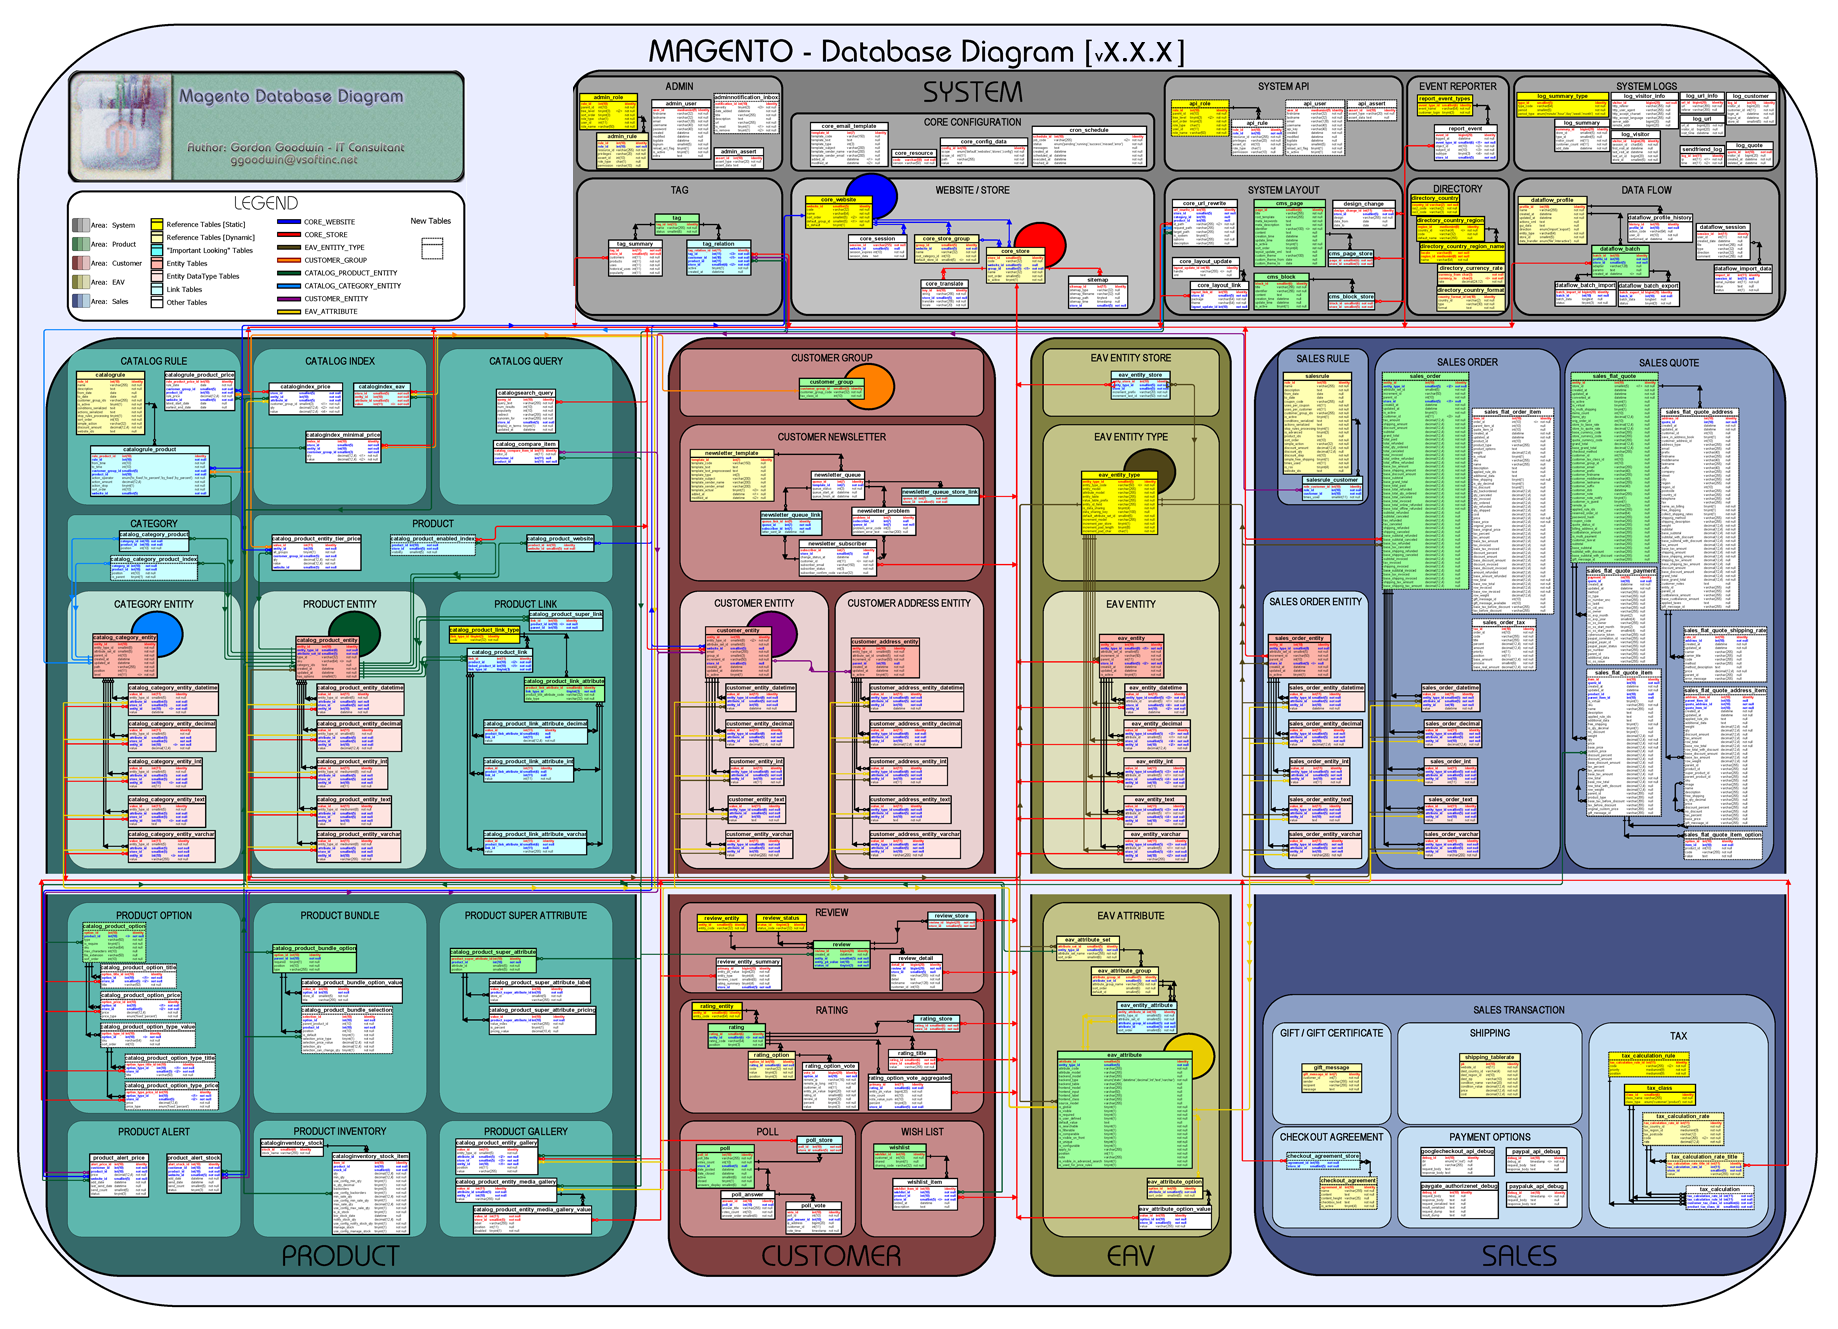
\includegraphics[width=0.8\textwidth]{figuras/apendice/magento_sample_database_diagram.png}
	\caption{\schemasDB de \nameMagento \ecommerceCOM \frameworkPC.}
	\label{ap:figure:catalog_magento}
\end{figure}

%\begin{figure}[h!]
%	\centering
%	\includegraphics[width=0.5\textwidth]{figuras/apendice/openCartWebsite.jpg}
%	\caption{\schemasDB de \ofBizNAME.}
%	\label{ap:figure:catalog_ofbiz}
%\end{figure}

%%%%%%%%%%%%%%%%%%%%%%%%%%%%%%%%%%%%%%%%%%%%%%%%%%%%%%%%%%%%%%%%%%%%%%%%%%%%%
%%%%%%%%%%%%%%%%%%%%%%%%%%%%%  Hadoop Meaning	%%%%%%%%%%%%%%%%%%%%%%%%%%%%%
%%%%%%%%%%%%%%%%%%%%%%%%%%%%%%%%%%%%%%%%%%%%%%%%%%%%%%%%%%%%%%%%%%%%%%%%%%%%%
\chapter{¿Qué es \hadoopNAME? \cite{online_hadoop_description}}\label{ap:apendice_hadoop_description}
\apacheNAME \hadoopNAME es un proyecto software \openSourcePC que permite el procesamiento distribuido de gran cantidad de datos a través de \clustersAS de \serversAS. Esta diseñado para \scaleUpQA desde un único \serverAS a miles de máquinas, con un muy alto grado de tolerancia al fallo. En lugar de confiar en \highEndCPT \hardwarePC, la flexibilidad de estos \clustersAS proviene de la habilidad del \softwarePC en detectar y manejar fallos en la \applayer.

\subsubsection*{Arquitectura \highLevelCPT} 
\apacheNAME \hadoopNAME tiene dos pilares:

\begin{itemize}
	\item \hadoopYarnNAME asigna \cpuPC, memoria y almacenamiento para las aplicaciones corriendo en \clustersAS \hadoopNAME. La primera generación de \hadoopNAME podía correr solo aplicaciones \hadoopMapReduceNAME. \hadoopYarnNAME permite que otros entornos de aplicaciones (como \sparkNAME) para ejecutarse en \hadoopNAME, lo que abre un mundo de posibilidades.
	
	\item \hadoophdfsNAME es un sistema de archivos que se extiende por todos los nodos en su \clusterAS \hadoopNAME para almacenamiento de datos. Se conecta entre si a los sistemas de archivos en muchos nodos locales para convertirlos en un sistema de archivos grandes.
\end{itemize}

\hadoopNAME se complementa con un ecosistema de proyectos de \apacheNAME, como Pig\cite{online_ibm_meaning_pig}, Hive\cite{online_ibm_meaning_hive} y Zookeeper\cite{online_ibm_meaning_zookeeper}, para extender el valor de \hadoopNAME y mejorar su \usabilityQA.


\subsubsection*{Entonces, ¿Cuál es el problema?}

\hadoopNAME cambia la economía y la dinámica de la computación a gran escala. Su impacto puede reducirse a cuatro características sobresalientes.

\hadoopNAME permite una solución de computación que es:

\begin{itemize}
	\item \textbf{\scalableQA}- Nuevos nodos pueden ser agregados según sean necesarios, y agregados sin la necesidad de cambiar el formato de los datos, como los datos son cargados, como los \textit{jobs} son escritos, o las aplicaciones en la parte superior.
	
	\item \textbf{\costEffectiveCPT}- \hadoopNAME trae computación paralela masiva a las maquinas de los servidores. El resultado es una considerable disminución en los costos por \terabytePC de almacenamiento. lo cual hace asequible para modelar todos sus datos.
	
	\item \textbf{\flexibleQA}- \hadoopNAME no tiene esquema, y puede absorber cualquier tipo de datos, estructurados o no, desde cualquier numero de fuentes. Los datos de múltiples fuentes pueden ser unidos y se agregan arbitrariamente para permitir análisis que ningún otro sistema puede proporcionar.
	
	\item \textbf{\faultTolerantQA}- Cuando se pierde un nodo, el sistema redirige el trabajo a otra ubicación de los datos para seguir con el procesamiento sin perder el ritmo.
\end{itemize}

%%%%%%%%%%%%%%%%%%%%%%%%%%%%%%%%%%%%%%%%%%%%%%%%%%%%%%%%%%%%%%%%%%%%%%%%%%%%%
%%%%%%%%%%%%%%%%%%%%%%    Stateful Stateless Meaning   %%%%%%%%%%%%%%%%%%%%%%
%%%%%%%%%%%%%%%%%%%%%%%%%%%%%%%%%%%%%%%%%%%%%%%%%%%%%%%%%%%%%%%%%%%%%%%%%%%%%
\chapter{Conexiones \statefulINT y \statelessINT }\label{ap:apendice_connection_statful_stateless}

Mantener el estado o ser \statefulINT significa que algunos dispositivos mantienen \trackCPT de otro dispositivo o una conexión, ya sea temporal o largo periodo de tiempo. Cuando se agrega el nombre de una persona en una libreta de direcciones y se observa su cumpleaños y teléfono, se podría decir que se esta manteniendo el estado de esa persona. En la \webINT una \cookieINT es un mecanismo \statefulINT que permite a los \webserverINT mantener \trackCPT de información de las personas, tal como se describe en un momento \cite{online_connection_stateful_stateless}.
%Keeping state or being stateful means that some device is keeping track of another device or a connection, either temporarily or over a long period of time. When I put someone's name in my address book and note their birthday and phone number, one could say that I am maintaining state for that person. On the Web, a cookie is a stateful mechanism that allows Web servers to keep track of information about people, as described in a moment.


Una conexión \statefulINT es una en la cual cierta información sobre una conexión entre dos sistemas es retenida para uso futuro. En algunos casos, la conexión es mantenida abierta incluso a través de dos sistemas que podrían no estar transmitiendo información(\ieCPT, la conexión en si misma mantiene el estado)\cite{online_connection_stateful_stateless}.
%A stateful connection is one in which some information about a connection between two systems is retained for future use. In some cases, the connection is kept open even though the two systems might not be transmitting information (i.e., the connection itself retains state).

En contraste, una conexión \statelessINT es aquella en que no hay información retenida por el \senderINT ó \receiverINT. El \senderINT transmite un paquete al \receiverINT sin esperar ninguna confirmación de recepción. El \receiverINT recibe el paquete sin ninguna configuración de la conexión anterior  \cite{online_connection_stateful_stateless}.
%In contrast, a stateless connection is one in which no information is retained by either sender or receiver. The sender transmits a packet to the receiver and does not expect an acknowledgment of receipt. The recipient receives the packet without any prior connection setup.


%%%%%%%%%%%%%%%%%%%%%%%%%%%%%%%%%%%%%%%%%%%%%%%%%%%%%%%%%%%%%%%%%%%%%%%%%%%%%
%%%%%%%%%%%%%%%%%%%%%%%%%%%%% Data Model Actual	%%%%%%%%%%%%%%%%%%%%%%%%%%%%%
%%%%%%%%%%%%%%%%%%%%%%%%%%%%%%%%%%%%%%%%%%%%%%%%%%%%%%%%%%%%%%%%%%%%%%%%%%%%%
%\chapter{ Avances \dataModelAS }\label{ap:avance_data_model}

\section{\itemcollection}

La estructura de \itemcollection se encuentra en \refsource{source:javascript:data_model_item}.

\medskip
\begin{lstlisting}[caption= \dataModelAS de \itemcollection, label=source:javascript:data_model_item]
	{
	    "_id" : "BCTMZ6HTxFSppJESk",
	    "createdAt" : ISODate("2014-04-03T20:46:52.411Z"),
	    "description" : "This is an example product.",
	    "hashtags" : [ 
	        "rpjCvTBGjhBi2xdro", 
	        "cseCBSSrJ3t8HQSNP"
	    ],
	    "isVisible" : true,
	    "metafields" : [ 
	        {
	            "key" : "Material",
	            "value" : "Cotton"
	        }, 
	        {
	            "key" : "Quality",
	            "value" : "Excellent"
	        }
	    ],
	    "pageTitle" : "Basic Example Product",
	    "productType" : "Simple",
	    "shopId" : "WvrKDomkYth3THbDD",
	    "title" : "Example Product",
	    "updatedAt" : ISODate("2015-06-01T19:17:13.949Z"),
	    "variants" : [],
	    "vendor" : "Example Manufacturer"
	}
\end{lstlisting}

El atributo \textit{'variants'} corresponde a un \arrayPL que contiene cada una de las modificaciónes que el \itemCOM tiene duranto su vida. Como ejemplo en \refsource{source:javascript:data_model_item_variant} se observa que el atributo \textit{'inventoryQuantity'} disminuye de 49 a 45 \itemsCOM.

\medskip
\begin{lstlisting}[caption= El \arrayPL "variants", label=source:javascript:data_model_item_variant]
	 "variants" : [ 
        {
            "_id" : "6qiqPwBkeJdtdQc4G",
            "title" : "Basic Example Variant",
            "price" : 19.99,
            "inventoryManagement" : true,
            "updatedAt" : ISODate("2015-04-03T20:46:52.411Z"),
            "createdAt" : ISODate("2015-04-03T20:46:52.411Z"),
            "inventoryQuantity" : 49,
            "metafields" : [ 
                {
                    "key" : null,
                    "value" : null
                }
            ]
        }, 
        {
            "_id" : "SMr4rhDFnYvFMtDTX",
            "title" : "Basic Example Variant",
            "price" : 19.99,
            "inventoryManagement" : true,
            "updatedAt" : ISODate("2014-05-03T20:46:52.411Z"),
            "createdAt" : ISODate("2014-05-03T20:46:52.411Z"),
            "inventoryQuantity" : 45,
            "metafields" : [ 
                {
                    "key" : null,
                    "value" : null
                }
            ]
        }
    ]
\end{lstlisting}



\section{\rolCollection}

\medskip
\begin{lstlisting}[caption= \dataModelAS de \rolCollection, label=source:javascript:data_model_roll]
	{
	    "name" : "admin",
	    "_id" : "vM2kbt4qCsZw7MbzK"
	}
\end{lstlisting}



\section{\userscollection}

\medskip
\begin{lstlisting}[caption= \dataModelAS de \userscollection, label=source:javascript:data_model_user]

{
    "_id" : "me8jP3idwNTecEkiD",
    "createdAt" : ISODate("2015-03-06T07:30:39.755Z"),
    "emails" : [ 
        {
            "address" : "yatkthjj@localhost",
            "verified" : false
        }
    ],
    "profile" : {},
    "roles" : [ 
        "manage-users", 
        "owner", 
        "admin"
    ],
   "username" : "Administrator"
}
\end{lstlisting}

\section{\tagscollection}

\medskip
\begin{lstlisting}[caption= \dataModelAS de \tagscollection, label=source:javascript:data_model_tag]

{
    "name" : "example-product",
    "updatedAt" : ISODate("2015-04-12T15:17:20.576Z"),
    "createdAt" : ISODate("2015-04-12T15:17:20.576Z"),
    "_id" : "cseCBSSrJ3t8HQSNP"
}

\end{lstlisting}


\section{\analyEventcollection}

\medskip
\begin{lstlisting}[caption= \dataModelAS de \analyEventcollection, label=source:javascript:data_model_analy_event]


{
    "category" : "grid",
    "action" : "generic-click",
    "label" : "product grid click",
    "shopId" : "WvrKDomkYth3THbDD",
    "_id" : "euGGJ2KQHvapX6rhk"
}

\end{lstlisting}

%%%%%%%%%%%%%%%%%%%%%%%%%%%%%%%%%%%%%%%%%%%%%%%%%%%%%%%%%%%%%%%%%%%%%%%%%%%%%
%%%%%%%%%%%%%%%%%%%%%%%%%%%%%  Pseudo Schemas	%%%%%%%%%%%%%%%%%%%%%%%%%%%%%
%%%%%%%%%%%%%%%%%%%%%%%%%%%%%%%%%%%%%%%%%%%%%%%%%%%%%%%%%%%%%%%%%%%%%%%%%%%%%
%\chapter{\pseudoSchemaCPT \ecommerceCOM }\label{ap:pseudo_schema_ecommerce}

\medskip
\begin{lstlisting}[caption= Busqueda en MongoDB, label=source:javascript:example_search_mongodb]

db.products.find({'_id': ObjectID("4bd87bd8277d094c458d2fa5")});

{
    _id         : ObjectID("4bd87bd8277d094c458d2a43"),
    title       : "A Love Supreme [Original Recording Reissued]"
    author      : "John Coltrane",
    author_id   : ObjectID("4bd87bd8277d094c458d2fa5"),
    details     : {
                    number_of_discs: 1,
                    label: "Impulse Records",
                    issue_date: "December 9, 1964",
                    average_customer_review: 4.95,
                    asin: "B0000A118M"
                },
    pricing     : {
                    list: 1198,
                    retail: 1099,
                    savings: 99,
                    pct_savings: 8
                },
   categories   : [
                    ObjectID("4bd87bd8277d094c458d2a43"),
                    ObjectID("4bd87bd8277d094c458d2b44"), 
                    ObjectID("4bd87bd8277d094c458d29a1")
                ]
}
\end{lstlisting}


\medskip
\begin{lstlisting}[caption= Estructura de una \orderCommerce., label=source:javascript:example_schema_order]

{
    '_id': objectid('4b980a6dea2c3f4579da141e'),
    'user_id': objectid('4b980a6dea2c3f4579a4f54'),
    'state': 'cart',
    'line_items': [
        {
            'sku': 'jc-432',
            'name': 'John Coltrane: A Love Supreme',
            'retail_price': 1099
        },
        {
            'sku': 'ly-211',
            'name': 'Larry Young: Unity',
            'retail_price': 1199
        }
    ],
    'shipping_address': {
        'street': '3333 Greene Ave.',
        'city': 'Brooklyn',
        'state': 'NY',
        'zip': '11216'
    },
    'subtotal': 2199
}
\end{lstlisting}

\medskip
\begin{lstlisting}[caption= Consulta eficiente con \secIndexesDB., label=source:javascript:example_querying_orders_mongodb]

    db.orders.ensureIndex({'line_items.sku': 1});
    db.orders.find({'line_items.sku' => 'jc-431'});
    
\end{lstlisting}



\medskip
\begin{lstlisting}[caption= Ejemplo de comando \mapReduce., label=source:javascript:example_aggregation_mongodb]

map = "
    function(){
        emit(this['shipping_address']['zip'], {total: this.total})
    }
"

reduce = "
    function(key, values) {
        var sum = 0;
        values.forEach(function(doc) {
      sum += doc.total;
    }

    return {total: sum};
  }"


db.orders.mapReduce(map, reduce, {out: 'order_totals_by_zip'});

\end{lstlisting}



\medskip
\begin{lstlisting}[caption= Ejemplo de uso de \positionOperatorDB., label=source:javascript:example_incrementing_quality_mongodb]

    db.orders.update(
        {
            '_id': order_id,
            'line_items.sku':'jc-431'
        },
        {
            '$set': {'line_items.$.quantity': 2}
        }
    );
        
\end{lstlisting}


\medskip
\begin{lstlisting}[caption= Ejemplo del operador \pushOperatorDB., label=source:javascript:example_push_operator_mongodb]
db.orders.update(
    {'_id': order_id},
    {
        '$push': {
            'line_items':{
                'sku': 'md-12',
                'price': 2500,
                'title': 'Basketball'
            }
        },
        '$inc': {'subtotal': 2500}
    }
);
\end{lstlisting}


\medskip
\begin{lstlisting}[caption= Ejemplo de \documentDB para un producto., label=source:javascript:example_document_inventory_mongodb]
{
    '_id': objectid('4b980a6dea2c3f4579da432a'),
    'sku': 'jc-431',
    'state': 'available',
    'expires': null,
    'order_id': null
}
\end{lstlisting}


\medskip
\begin{lstlisting}[caption= Marcando un producto con tiempo de espiración., label=source:javascript:example_add_inventory_expiartion_mongodb]
query = {'sku': 'jc-431', 'state': 'available'};

update = {
    '$set':{
        'state': 'cart',
        'order_id': order_id,
        'expires':  Date.now() + 15 * 60
    }
};

item = db.inventory.findAndModify(query: query, update: update);
\end{lstlisting}


\medskip
\begin{lstlisting}[caption= Ejemplo de \scriptPL corriendo \backgroundPL., label=source:javascript:example_add_script_background_mongodb]
db.inventory.update(
    {
        'state': 'cart',
        'expires': {'$lt': Date.now()}},
        {
            '$set': {
                'state': 'available',
                'expires': null,
                'order_id': null
        }
    },
    {multi: true}
);
\end{lstlisting} 


%%%%%%%%%%%%%%%%%%%%%%%%%%%%%%%%%%%%%%%%%%%%%%%%%%%%%%%%%%%%%%%%%%%%%%%%%%%%%
%%%%%%%%%%%%%%%%%%%%%%%%%%%%     Formularios	 %%%%%%%%%%%%%%%%%%%%%%%%%%%%
%%%%%%%%%%%%%%%%%%%%%%%%%%%%%%%%%%%%%%%%%%%%%%%%%%%%%%%%%%%%%%%%%%%%%%%%%%%%%
%!TEX root = ../../memoria.tex
\chapter{\uiSiglaAS de los formularios}\label{ap:ui:forms}

%!TEX root = ../../../memoria.tex

\begin{figure}[H]
	\centering
	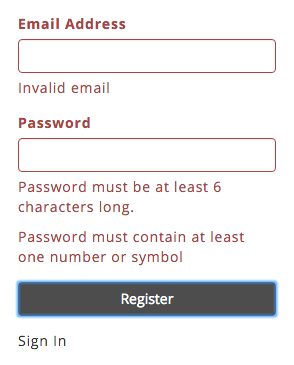
\includegraphics[width=0.6\textwidth]{figuras/architecture/accounts/new/send_error.png}
	\caption{Errores al enviar el formulario de creación de una nueva cuenta.}
	\label{figure:architecture:accounts:new:send_error}
\end{figure}

\begin{figure}[H]
	\centering
	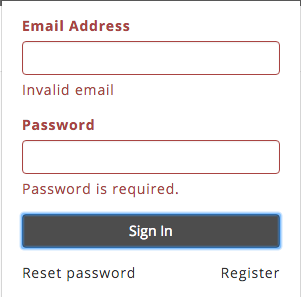
\includegraphics[width=0.6\textwidth]{figuras/architecture/accounts/signin/send_empty.png}
	\caption{Errores al enviar vacio el formulario de autenticación.}
	\label{figure:architecture:accounts:signin:send_empty}
\end{figure}

%!TEX root = ../../../memoria.tex
\begin{figure}[H]
	\centering
	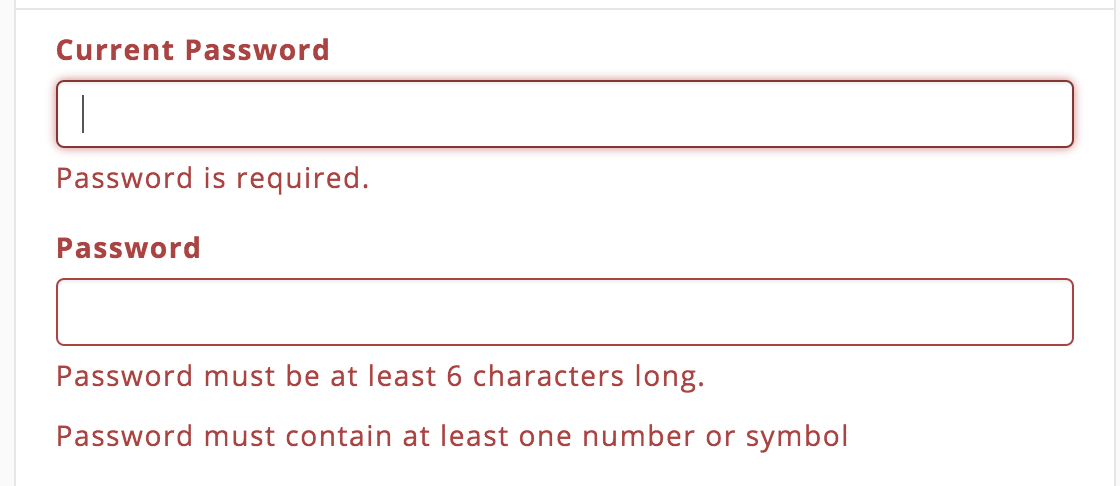
\includegraphics[width=0.8\textwidth]{figuras/formularios/update_password/empty_form_send.png}

	\caption{Errores del formulario de actualización de contraseña tras enviarlo vacío.}
	\label{figure:apendice:profile:form:update_password:empty_form_send}
\end{figure}

\begin{figure}[H]
	\centering
	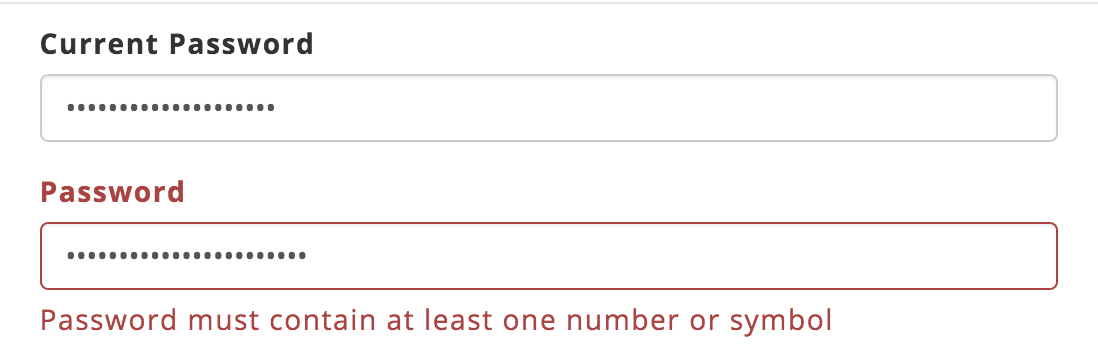
\includegraphics[width=0.8\textwidth]{figuras/formularios/update_password/weak_password.png}

	\caption{Ingreso de nueva \textit{contraseña fácil}.}
	\label{figure:apendice:profile:form:update_password:week_password}
\end{figure}


\begin{figure}[H]
	\centering
	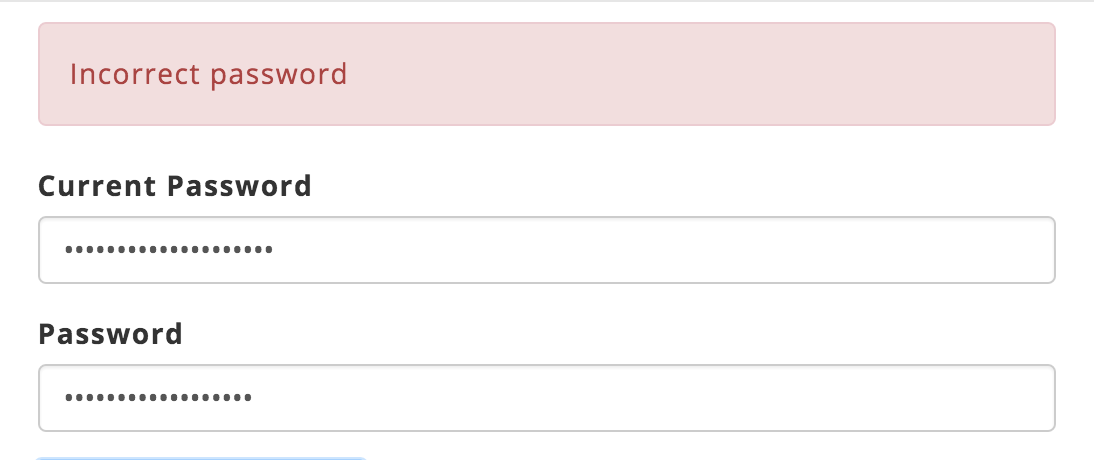
\includegraphics[width=0.7\textwidth]{figuras/formularios/update_password/incorrect_password.png}

	\caption{Ingreso de contraseña actual incorrecta.}
	\label{figure:apendice:profile:form:update_password:incorrect_password}
\end{figure}

%!TEX root = ../../../memoria.tex

\begin{figure}[H]
	\centering
	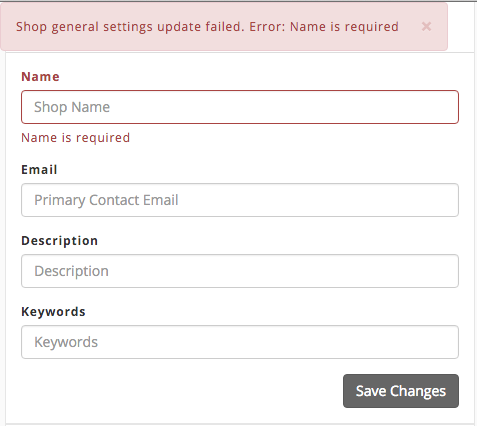
\includegraphics[width=0.6\textwidth]{figuras/dashboard/ecommerce/general_menu/updated_error.png}
	\caption{Errores en el formulario tras enviarlo. El campo \textit{Name} es obligatorio.}
	\label{figure:apendice:dashboard:ecommerce:general_menu:updated_error}
\end{figure}

\begin{figure}[H]
	\centering
	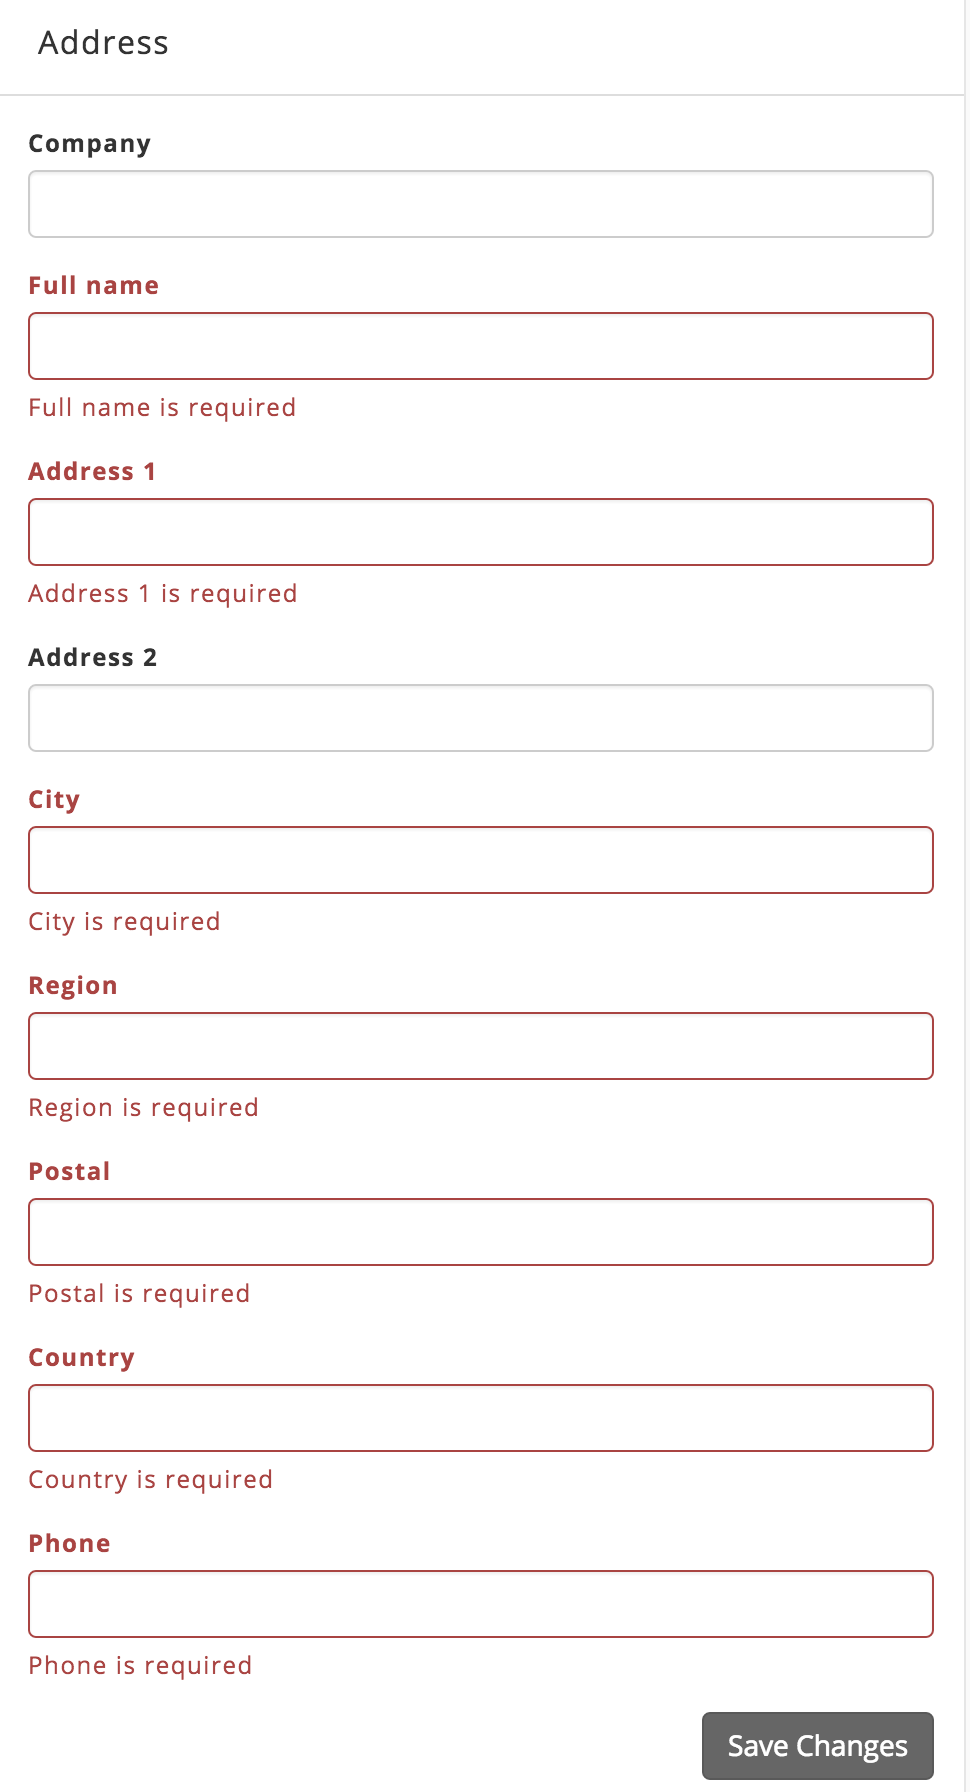
\includegraphics[width=0.5\textwidth]{figuras/dashboard/ecommerce/address/updated_error.png}
	\caption{Comentarios del formulario tras error de actualización.}
	\label{figure:apendice:dashboard:ecommerce:address:updated_error}
\end{figure}

\begin{figure}[H]
	\centering
	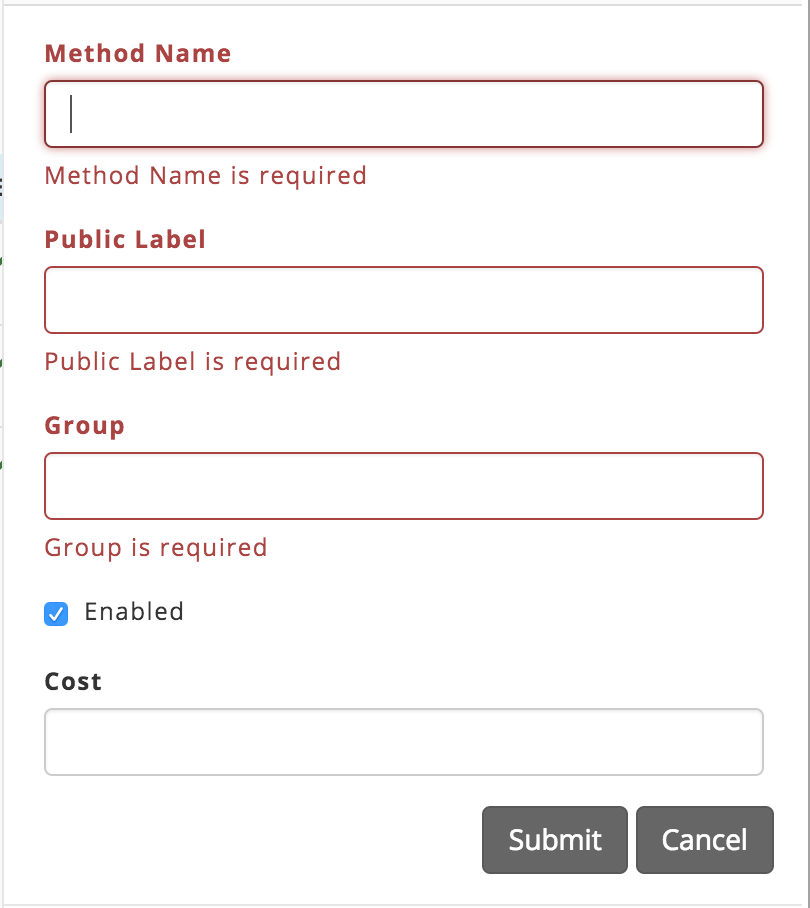
\includegraphics[width=0.6\textwidth]{figuras/dashboard/shipping/form_shipping_add_send_empty.png}
	\caption{Formulario de creación de \shippingEF tras enviarlo vacío.}
	\label{figure:apendice:dashboard:shipping:form_shipping_add_send_empty}
\end{figure}





%%%%%%%%%%%%%%%%%%%%%%%%%%%%%%%%%%%%%%%%%%%%%%%%%%%%%%%%%%%%%%%%%%%%%%%%%%%%%
%%%%%%%%%%%%%%%%%%%%%%%%%%%%    Good Practices	 %%%%%%%%%%%%%%%%%%%%%%%%%%%%
%%%%%%%%%%%%%%%%%%%%%%%%%%%%%%%%%%%%%%%%%%%%%%%%%%%%%%%%%%%%%%%%%%%%%%%%%%%%%
%!TEX root = ../../memoria.tex
\chapter{Soluciones de otras plataformas \ecommerceCOM}\label{ap:goodPractices:ecommerce}

%!TEX root = ../../../memoria.tex

\begin{figure}[H]
	\centering
	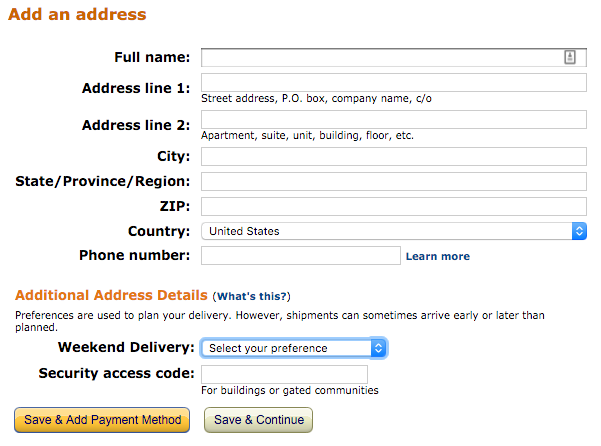
\includegraphics[width=0.6\textwidth]{figuras/address/examples/amazon_address.png}
	\caption{Formulario para agregar una dirección en \amazonNAME.}
	\label{figure:apendice:address:example:amazon_address}
\end{figure}


%!TEX root = ../../../memoria.tex

\begin{figure}[H]
	\centering
	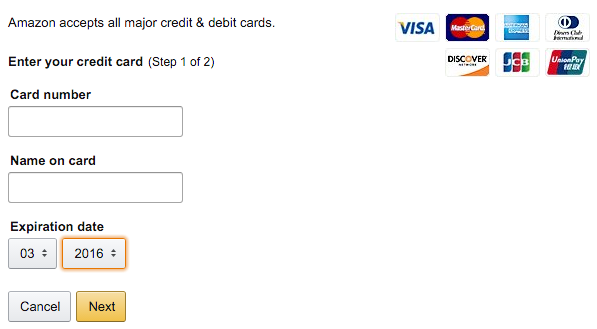
\includegraphics[width=0.6\textwidth]{figuras/creditCard/examples/amazon_add_card.png}
	\caption{Formulario de \amazonNAME para agregar una tarjeta.}
	\label{figure:apendice:creditCard:example:amazon_add_card}
\end{figure}

\begin{figure}[H]
	\centering
	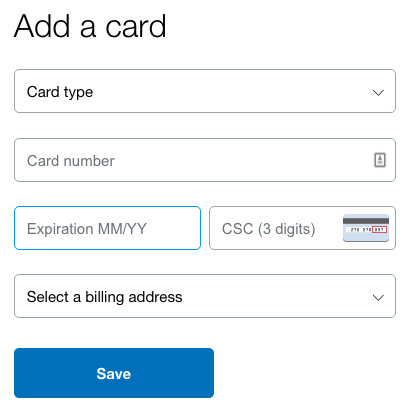
\includegraphics[width=0.6\textwidth]{figuras/creditCard/examples/paypal_add_card.png}
	\caption{Formulario de \paypalNAME para agregar una tarjeta.}
	\label{figure:apendice:creditCard:example:paypal_add_card}
\end{figure}

%!TEX root = ../../../memoria.tex

\begin{figure}[H]
	\centering
	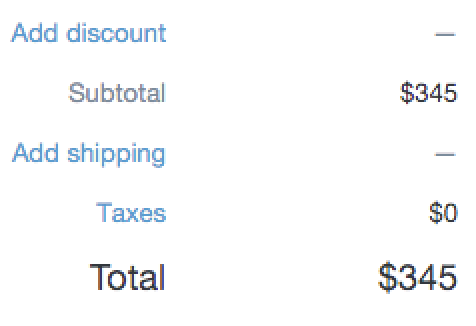
\includegraphics[width=0.4\textwidth]{figuras/cart/examples/cart_summarize_shopify.png}
	\caption{Resumen del carro de compra del sitio \shopifyNAME.}
	\label{figure:apendice:cart:example:cart_summarize_shopify}
\end{figure}

\end{document}